%###
% \RequirePackage[l2tabu, orthodox]{nag}
\documentclass[a4paper,10pt,twoside]{book}
% \usepackage[width=127mm,height=191mm,includehead,hcentering,vcentering]{geometry}

% \includeonly{_init,basic-concepts,raster}
% \includeonly{__init,k3tree}

% Packages --------------------------------------------------------------------

\usepackage{booktabs,multirow,multicol,array,colortbl,makecell,tabularx} % tablas


\usepackage[width=127mm,height=191mm,includehead,hcentering,vcentering]{geometry}
\usepackage{graphicx,subfigure}				% Include graphics
\usepackage{caption}	% Customize captions
\usepackage[T1]{fontenc} 			% Extended character set
\usepackage{lmodern, microtype}		% Load vector fonts; better text formatting
\usepackage{amsmath,amssymb,amsfonts,amsthm}	% Math support, example environment
\usepackage{fancyhdr} 				% Headers
\usepackage{xspace}	  				% Create macros with appropriate extra space after
\usepackage{lipsum}					% Fill sections
\usepackage{fixltx2e}				% Make math macros robust: \( \) \[ \]



\usepackage[usenames,dvipsnames]{xcolor}	% Colors

\usepackage[chapter]{algorithm}
\usepackage{algorithmicx, algpseudocode}
\usepackage{float}

\usepackage{textcomp, gensymb}	% Common symbols (mu, degree)

%Debug packages
% \usepackage{refcheck}	% Show labels in output pdf. 
						% Note: local refcheck.sty has been modified to solve a bug in handling bibitems 
						% Note 2: since cleveref refcheck is unused




\usepackage{tikz}

\usepackage[breaklinks]{hyperref} % Hyperlinks in refs. Must be loaded at the end (except cleverref)
\usepackage{hypdvips}
% \usepackage[nameinlink]{cleveref}
\usepackage{cleveref}

% \usepackage{theorem}					% Theorems?
% \theoremstyle{plain}
% \newtheorem{definition}{Definition}

% \usepackage{lscape} 					% Set elements to landscape (e.g large figures, tables)
% \usepackage{setspace}					% ??
% \usepackage{rotating}
% \usepackage[tight]{subfigure}
% \usepackage{dcolumn}
% \usepackage[noline,linesnumbered,algochapter]{algorithm2e}
% \providecommand{\DontPrintSemicolon}{\dontprintsemicolon}
% \usepackage{algcompatible}
% \usepackage{sectsty}
%\usepackage[none]{hyphenat}
% \usepackage[tworuled,noline,linesnumbered,algochapter]{algorithm2e}


% FIXME: review in further versions
\hyphenpenalty=5000
\tolerance=1000
\widowpenalty=300
\clubpenalty=300
\emergencystretch=3em

\hfuzz=3em

\usepackage{etoolbox}
\apptocmd{\sloppy}{\hbadness 10000\relax}{}{}	% Avoid ''underfull hbox'' warnings in bibliography


% Separacion entre un parrafo y el siguiente
% \addtolength{\smallskipamount}{-7.60pt}
% \addtolength{\parskip}{.5\baselineskip}%{.5\baselineskip}

% \setlength{\smallskipamount}{-7.60pt}
% \setlength{\parskip}{\smallskipamount}

% Fuente de las subsubsecciones
%\subsubsectionfont{\bf}

\setcounter{tocdepth}{4} \setcounter{secnumdepth}{4}

% Fuentes de los pies de figura
\renewcommand{\captionlabelfont}{\bfseries}
\setlength{\captionmargin}{\parindent}

\renewcommand{\arraystretch}{1.2}	% Adjust vertical margins in tables

%Comandos

\newcounter{example}[chapter]
\def\theexample{\thechapter.\arabic{example}}
\newenvironment{example}{\par\noindent\textbf{Example \refstepcounter{example}\theexample:}}{}

% I need subsubsubsections, but not in the index
\newcommand{\subsubsubsection}[1]{\vspace{2mm}\par\noindent\textbf{#1}}

\renewcommand{\algorithmicrequire}{\textbf{Input:}}
\renewcommand{\algorithmicensure}{\textbf{Output:}}
\newcommand{\Input}{\Require}
\newcommand{\Output}{\Ensure}
\newcommand{\false}{\textbf{false}}
\newcommand{\red}[1]{{\color{red} #1 }}
\newcommand{\blue}[1]{{\color{blue} #1 }}
\newcommand{\cyan}[1]{{\color{cyan} #1 }}
\newcommand{\green}[1]{{\color{green} #1 }}
\newcommand{\todo}[1]{\blue{#1}}
\newcommand{\rewrite}[1]{\cyan{#1}}
\newcommand{\fixme}[1]{{\Large \red{#1}}}

\newcommand*{\irank}[0]{\emph{rank}\xspace}
\newcommand*{\iselect}[0]{\emph{select}\xspace}
\newcommand*{\iaccess}[0]{\emph{access}\xspace}

\DeclareMathOperator\rank{rank}
\DeclareMathOperator\select{select}
\DeclareMathOperator\access{access}

\renewcommand*{\k}[0]{\ensuremath{K}\xspace}
\newcommand*{\kk}[0]{\ensuremath{\k^2}\xspace}
\newcommand*{\kkk}[0]{\ensuremath{\k^3}\xspace}
\newcommand*{\KK}[0]{\ensuremath{\K^2}\xspace}
\newcommand*{\Ktree}[0]{\ensuremath{\k^2}-tree\xspace}
\newcommand*{\ktree}[0]{\ensuremath{\k^2}-tree\xspace}
\newcommand*{\ktrees}[0]{\ensuremath{\k^2}-trees\xspace}
\newcommand*{\Ktrees}[0]{\ensuremath{\k^2}-trees\xspace}
\newcommand*{\koct}[0]{\ensuremath{\k^3}-tree\xspace}
\newcommand*{\Koct}[0]{\ensuremath{\k^3}-tree\xspace}
\newcommand*{\kntree}[0]{\ensuremath{\k^n}-tree\xspace}
\newcommand*{\Kntree}[0]{\ensuremath{\k^n}-tree\xspace}
\newcommand{\kones}[0]{\ensuremath{\k^2}-tree1\xspace}
\newcommand{\koness}[0]{\ensuremath{\k^2}-tree1s\xspace}
\newcommand{\Kones}[0]{\kones}
\newcommand{\kdouble}[0]{\ensuremath{\k^2}-tree1\ensuremath{^{\mathrm{2bits-naive}}}\xspace}
\newcommand{\ksus}[0]{\ensuremath{\k^2}-tree1\ensuremath{^{\mathrm{2bits}}}\xspace}
\newcommand{\kdf}[0]{\ensuremath{\k^2}-tree1\ensuremath{^{\mathrm{df}}}\xspace}
\newcommand{\klevel}[0]{\ensuremath{\k^2}-tree1\ensuremath{^{\mathrm{1-5 bits}}}\xspace}
\newcommand{\Kdouble}[0]{\kdouble}
\newcommand{\Ksus}[0]{\ksus}
\newcommand{\Kdf}[0]{\kdf}
\newcommand{\Klevel}[0]{\klevel}
\newcommand{\btree}[0]{B-tree\xspace}
\newcommand{\btrees}[0]{B-trees\xspace}
\newcommand{\bplus}[0]{B\ensuremath{^+}-tree\xspace}
\newcommand{\bpluss}[0]{B\ensuremath{^+}-trees\xspace}
\newcommand{\dktree}[0]{d\ktree}
\newcommand{\dktrees}[0]{d\ktrees}
\newcommand{\Dktree}[0]{D\ktree}
\newcommand{\Dktrees}[0]{D\dtrees}
\newcommand{\iktree}{I\ktree}
\newcommand{\diktree}{diff-I\ktree}
\newcommand{\mktree}{M\ktree}

\newcommand{\kkind}{M\kones}
\newcommand{\kkacum}{AM\kones}
\newcommand{\ikones}{I\kones}
\newcommand{\koctindex}{\koct}

\newcommand{\diffk}[0]{diffK}
\newcommand{\ediffk}[0]{enh-diffK}
\newcommand{\Diffk}[0]{DiffK}
\newcommand{\Ediffk}[0]{Enh-diffK}

\newcommand{\ktreap}[0]{\ensuremath{\k^2}-treap\xspace}
\newcommand{\ktreaps}[0]{\ensuremath{\k^2}-treaps\xspace}

\newcommand{\ZERO}[0]{0\xspace}
\newcommand{\ZEROS}[0]{0's\xspace}
\newcommand{\ONE}[0]{1\xspace}
\newcommand{\ONES}[0]{1s\xspace}

\newcommand{\dash}[0]{\text{--}}

\newcommand{\kt}[0]{\ensuremath{k}\xspace}

\newcommand{\tdktree}[0]{tt\ktree}


\crefname{algorithm}{Algorithm}{Algorithms}
\crefname{example}{Example}{Examples}
\crefname{part}{Part}{Parts}
\crefname{table}{Table}{Tables}

% \normalfont
% \DeclareFontShape{T1}{lmr}{bx}{sc} { <-> ssub * cmr/bx/sc }{}

\normalfont
\DeclareFontShape{T1}{lmr}{bx}{sc} { <-> ssub * cmr/bx/sc }{}

%%%%%%%%%%%%%%%%%%%%%%%%%%%%%%%%%%%%%%%%%%%%%%%%%%%%%%%%%%%
%%%%%%%%%%%%%%%% Sandbox
% \DeclareSymbolFont{sfoperators}{OT1}{cmss}{m}{n}
% \DeclareSymbolFontAlphabet{\mathsf}{sfoperators}
% 
% \makeatletter
% % \def\operator@font{\mathgroup\symsfoperators}
% \def\select@font{\mathgroup\symsfoperators}
% \makeatother
% 
% \makeatletter
% \def\rank@font{\sf}
% \def\select@font{\bf}
% \makeatother

% \newcommand{\rank}[0]{\ensuremath{\mathrm{rank}}\xspace}
% \newcommand{\select}[0]{\ensuremath{\mathrm{select}}\xspace}
% \newcommand{\irank}[0]{\emph{rank}\xspace}
% \newcommand{\iselect}[0]{\emph{select}\xspace}
% \def\rank{\ensuremath{\mathsf{rank}}}
% \def\select{\ensuremath{\mathsf{select}}}
% \DeclareMathOperator\rank{rank}
% \DeclareMathOperator\select{select}

%%%%%%%%%%%%%% End sandbox
%%%%%%%%%%%%%%%%%%%%%%%%%%%%%%%%%%%%%%%%%%%%%%%%%%%%%

\makeglossaries

\begin{document}

%\epstopdfsetup{outdir=./}
\pagenumbering{roman}
\pagestyle{fancy}\fancyfoot{}\fancyhead{}
\fancyhead[LO]{\slshape\nouppercase{\rightmark}}
\fancyhead[RE]{\slshape\nouppercase{\leftmark}}
\fancyhead[RO,LE]{\slshape \thepage}

\frontmatter

\newacronym{afc}{AFC}{Automated Fare Collection}
\newacronym{gis}{GIS}{Geographic Information System}
\newacronym{csa}{CSA}{Compressed Suffix Array}
\newacronym{wt}{WT}{Wavelet Tree}
\newacronym{wm}{WM}{Wavelet Matrix}
\newacronym{htwt}{HTWT}{Hu-Tucker Wavelet Tree}
\newacronym{ctr}{CTR}{Compact Trip Representation}
\newacronym{gtfs}{GTFS}{General Transit Feed Specification}
\newacronym{sat}{SAT}{Summed Area Table}
\newacronym{ttctr}{TTCTR}{Topology\&Trip-aware Compact Trip Representation}
\newacronym{xctr}{XCTR}{eXtended Compact Trip Representation}
\newacronym{tm}{T-Matrices}{Trip-Matrices}
\newacronym{dbms}{DBMS}{Database Management System}
\newacronym{rdbms}{RDBMS}{Relational Database Management System}
\newacronym{wms}{WMS}{Web Map Service}
\newacronym{wfs}{WFS}{Web Feature Service}
\begin{titlepage}


\vspace*{0.9cm}

\noindent {\Huge Compressed Data Structures\\ for Trajectory Representation}

\vspace*{1.5cm}

\noindent {\huge Autor: Daniil Galaktionov Hodovaniuk}


\definecolor{rosaudc}{RGB}{198, 0, 126}
\noindent \textcolor{rosaudc}{\rule{\textwidth}{2mm}}

{\large
  \noindent Tesis doctoral UDC / 2019

  \vspace*{1.5cm}

  \noindent Directores: \\Antonio Fari\~na Mart\'inez \\ Nieves Rodr\'iguez Brisaboa
  
  \vspace*{1.0cm}
  
  \noindent Tutor y Director por parte de la empresa: \\Eduardo Rodr\'iguez L\'opez

  \vspace*{1.5cm}

 % \noindent Programa Oficial de Doutoramento en Computaci\'on
}

\begin{center}
  \vspace*{1.9cm}
  
\includegraphics[scale=0.20]{figures/_init/udc-color}
\end{center}


\end{titlepage}

\thispagestyle{empty}

%\begin{titlepage}
%\begin{center}
%
%%\vspace*{0.9cm}
%
%
\includegraphics[scale=0.30]{figures/_init/udc-color}
%
%\vspace*{1.2cm}
%
%%{\large \sc Departamento de Computaci\'on, Universidade da Coru\~na} \\[5mm]
%%{\large \scshape Departamento de Computaci\'on} \\[5mm]
%%{\large } \\[2mm]
%%{\Large \scshape Proyecto fin de carrera \\ de Ingenier�a Inform�tica} \\
%
%\vspace*{2.5cm}
%
%{\LARGE \textsc{\textbf Compact data structures for large and complex datasets}}
%
%\end{center}
%
%\vspace*{2.8cm}
%
%\begin{center}
%%\large \bf
%\large
%{\Large \textsc{\textbf{Tesis Doctoral}}} \\[1.8cm]
%{{Doctorando:}  %\\[2mm]
%Fernando Silva Coira}\\[4mm]
%{{Directores:} %\\[2mm]
%Susana Ladra Gonz\'alez, Jos\'e Ram\'on Param\'a Gab\'ia}\\[1.2cm]
%{A Coru\~na, Julio de 2017}
%\end{center}
%
%\end{titlepage}
%
%\thispagestyle{empty}

\begin{titlepage}


\vspace*{0.9cm}

\noindent {\Huge Trust me I'm a Doctor}

\vspace*{1.5cm}

\noindent {\huge Autor: Daniil Galaktionov Hodovaniuk}


\definecolor{rosaudc}{RGB}{198, 0, 126}
\noindent \textcolor{rosaudc}{\rule{\textwidth}{2mm}}

{\large
  \noindent Tesis doctoral UDC / 2019

  \vspace*{1.5cm}

  \noindent Directores: \\Antonio Fari\~na Mart\'inez \\ Nieves Rodr\'iguez Brisaboa
  
  \vspace*{1.5cm}

  \noindent Programa Oficial de Doutoramento en Computaci\'on
}

\begin{center}
  \vspace*{1.9cm}
  
\includegraphics[scale=0.20]{figures/_init/udc-color}
\end{center}


\end{titlepage}

\thispagestyle{empty}

%\begin{titlepage}
%\begin{center}
%
%%\vspace*{0.9cm}
%
%
\includegraphics[scale=0.30]{figures/_init/udc-color}
%
%\vspace*{1.2cm}
%
%%{\large \sc Departamento de Computaci\'on, Universidade da Coru\~na} \\[5mm]
%%{\large \scshape Departamento de Computaci\'on} \\[5mm]
%%{\large } \\[2mm]
%%{\Large \scshape Proyecto fin de carrera \\ de Ingenier�a Inform�tica} \\
%
%\vspace*{2.5cm}
%
%{\LARGE \textsc{\textbf Compact data structures for large and complex datasets}}
%
%\end{center}
%
%\vspace*{2.8cm}
%
%\begin{center}
%%\large \bf
%\large
%{\Large \textsc{\textbf{Tesis Doctoral}}} \\[1.8cm]
%{{Doctorando:}  %\\[2mm]
%Fernando Silva Coira}\\[4mm]
%{{Directores:} %\\[2mm]
%Susana Ladra Gonz\'alez, Jos\'e Ram\'on Param\'a Gab\'ia}\\[1.2cm]
%{A Coru\~na, Julio de 2017}
%\end{center}
%
%\end{titlepage}
%
%\thispagestyle{empty}

\pagebreak \mbox{} \pagebreak
\thispagestyle{empty}

\begin{flushleft}

{\bfseries PhD thesis supervised by} \\[1pt]
{\itshape \bfseries Tesis doctoral dirigida por} \\[4mm]

{\bfseries Antonio Fari\~na Mart\'inez} \\[2pt]
Departamento de Computaci\'on \\[1pt]
Facultad de Inform\'atica \\[1pt]
Universidade da Coru\~na \\[1pt]
15071 A Coru\~na (Espa\~na) \\[1pt]
Tel: +34 981 167000 ext. 1352 \\[1pt]
Fax: +34 981 167160 \\[1pt]
\verb=antonio.farina@udc.es= \\[4mm]

{\bfseries Nieves Rodr\'iguez Brisaboa} \\[2pt]
Departamento de Computaci\'on \\[1pt]
Facultad de Inform\'atica \\[1pt]
Universidade da Coru\~na \\[1pt]
15071 A Coru\~na (Espa\~na) \\[1pt]
Tel: +34 981 167000 ext. 1243 \\[1pt]
Fax: +34 981 167160 \\[1pt]
\verb=brisaboa@udc.es= \\[8mm]

{\itshape \bfseries Tutor y director responsable por parte de la empresa} \\[4mm]

{\bfseries Eduardo Rodr\'iguez L\'opez} \\[2pt]
%Tutor y Director responsable por parte de la empresa \\[1pt]
Enxenio S.L. \\[1pt]
Calle Jos\'e Luis Bugallal Marchesi \\[1pt]
\textnumero~20 1 Izq., 15008 A Coru\~na (Espa\~na) \\[1pt]
Tel: +34 981 913 768 \\[1pt]
\verb=edu@enxenio.es=

\end{flushleft}

Antonio Fari\~na, Nieves Rodr\'iguez Brisaboa y Eduardo Rodr\'iguez, como directores, acreditamos que esta tesis cumple los requisitos para optar a los t\'itulo de doctor industrial e internacional, y autorizamos su dep\'osito y defensa por parte de Daniil Galaktionov Hodovaniuk cuya firma tambi\'en se incluye.




\thispagestyle{plain}
\pagebreak \mbox{} \pagebreak

\vspace*{\stretch{1}}
\begin{flushright} \large \itshape

In the memory of my grandmother.

\end{flushright}
\vspace*{\stretch{1}}

\thispagestyle{empty}

\thispagestyle{plain}
\chapter*{Acknowledgements}
Extended acknowledgements.\\

\vspace*{\fill}
This thesis has received funding from ...

\chapter*{Agradecimientos}
Dedicatoria larga.\\

\vspace*{\fill}
Esta tesis ha recibido fondos ...
\thispagestyle{plain}

\chapter*{Abstract}

The proliferation of GPS devices in smartphones, vehicles and sport wearables on the one hand, and geolocation mechanisms (such as smart cards in public transportation) on the other hand, have led to an unprecedented ability to gather and store trajectories that originate from people's movements during their daily schedules. However, no standard data models exist to represent these trajectories and, in addition, neither traditional databases nor new \textit{NoSQL} databases are adequate for the representation and exploitation of the complex spatio-temporal data that make up such trajectories. This general outlook is even more complex once we consider that whenever we are storing information related to the context of public transportation passengers, customers inside a mall, or simply vehicles moving in a city we must deal with a true Big Data scenario in which guaranteeing an efficient response can be very challenging.

Consequently, in this thesis we address the design of compact data structures for the representation of the followed trajectories, both in the context of vehicles and/or people moving in urban or periurban spaces, as in the context of itineraries of commuters in public transportation. Apart from designing these compact data structures that allow us to represent the Big Data scenario usually seen in this application domain, we have also designed the algorithms that allow the efficient exploitation of the underlying information.

We have implemented algorithms that not only to solve the classic spatio-temporal queries, such as obtaining the position of a moving object at a time instant, reconstructing the trajectory of an object, or even spatio-temporal window queries (which objects are inside a spatial range either within a time window or at a time instant), but also solve more specialized queries for the analysis of the trajectories that travelers make. For instance, we have designed algorithms to query the number of travelers that start (or finish) their trip in a certain place within a given time interval, or the number of travelers that switch from one line from the public transportation network to another one using a particular stop, or even the number of travelers that had started their trip in a certain place (which can be either a stop or a whole neighborhood) and finished it in another place.

Both the designed structures and the querying algorithms, which are available at \url{https://github.com/dgalaktionov/compact-trip-representation}, have been experimentally evaluated. With these structures we were able to represent, in a compact space of 100 MiB, a collection of approximately a million and a half of taxi trajectories, or alternatively ten million trajectories consisting of itineraries over public transportation networks (the latter being more compressible). In both cases, we can solve most of the considered exploitation queries in the order of microseconds, with algorithms that scale logarithmically with respect to the increase in the number of stored trajectories.

Finally, considering that this work is considered an industrial thesis, and that this requires showing that the research performed is of clearly applied nature, we have developed a web application with Geograhic Information Systems technology, which integrates with our compressed structures and algorithms instead of relying on common spatial databases. This application, which provides a simple and intuitive user interface that represents the map of a transportation network, enabled an end user to run the aforementioned querying algorithms over a large collection of historic trajectories. Likewise, this interface presents the query results in a graphical and intuitive way.

\chapter*{Resumen}

La proliferaci\'on de por un lado de dispositivos GPS en smartphones, veh\'iculos o pulseras de deporte,  y por otro, de otros mecanismos de geolocalizaci\'on (como las tarjetas de pago de trasporte p\'ublico), han dado lugar a una capacidad in\'edita de obtener y almacenar las trayectorias que generan las personas al moverse durante sus quehaceres diarios. Sin embargo, no existen modelos de datos est\'andar para representar dichas trayectorias, adem\'as de que ni las bases de datos tradicionales, ni las nuevas bases de datos \textit{NoSQL} se adec\'uan bien a la representaci\'on y explotaci\'on de esos datos complejos de naturaleza espacio-temporal que son las trayectorias.  Para hacer m\'as complejo a\'un el panorama, se constata adem\'as que cuando se quieren almacenar trayectorias de viajeros de transporte p\'ublico, o de clientes en centros comerciales, o simplemente de personas o veh\'iculos movi\'endose por una ciudad hay que enfrentarse a un verdadero escenario Big Data en el que la eficiencia en la respuesta a las consultas se hace muy dif\'icil.

Por todo ello, en esta tesis se aborda el dise\~no de estructuras de datos compactas para la representaci\'on de las trayectorias seguidas, por un lado, por veh\'iculos y/o personas que se mueven por las calles de un entorno urbano o periurbano acotado, y por otro los itinerarios de viajeros de transporte p\'ublico. Adem\'as de dise\~nar esas estructuras de datos compactas, que permiten representar ese escenario Big Data habitual en estos dominios de aplicaci\'on, se han dise\~nado los algoritmos que permiten la explotaci\'on eficiente de dichos datos.

Hemos implementado algoritmos que, adem\'as de resolver las consultas espacio-temporales cl\'asicas, tanto las de posici\'on de un objeto en un tiempo, o trayectoria de un objeto durante un intervalo temporal, como las consultas de rango espacio-temporal (qu\'e objetos est\'an en una ventana del espacio en un instante o intervalo temporal) resuelven tambi\'en consultas m\'as especializadas para el an\'alisis de trayectorias de viajeros. Por ejemplo, hemos dise\~nado algoritmos para  consultar el n\'umero de viajeros que inician (o terminan)  su viaje en un lugar dado dentro de un cierto intervalo temporal, o el n\'umero de viajeros que conmutan de una l\'inea a otra de la red de transporte p\'ublico en una parada concreta, o incluso el n\'umero de viajeros que inicia su viaje en cierto lugar (parada o  barrio) y lo termina en otra parada o barrio determinados. 

Tanto las estructuras de datos dise\~nadas como todos los algoritmos de consulta,  que  est\'an disponibles en \url{https://github.com/dgalaktionov/compact-trip-representation},  han sido evaluados experimentalmente. Con estas estructuras es posible representar en un espacio de 100 MiB una colecci\'on de aproximadamente un mill\'on y medio de trayectorias de taxis, o alternativamente diez millones de trayectorias consistentes de itinerarios sobre redes de transporte p\'ublico, al ser \'estas \'ultimas m\'as compactas. En ambos casos, podemos resolver la mayor parte de las consultas de explotaci\'on planteadas en el orden de microsegundos, con algoritmos que escalan de forma logar\'itmica con respecto al incremento en el n\'umero de trayectorias almacenadas.

Por \'ultimo, considerando que este trabajo est\'a considerado como una tesis industrial, lo cual requiere demostrar que el trabajo investigador realizado es de naturaleza aplicada, hemos desarrollado una aplicaci\'on web con tecnolog\'ia de Sistemas de Informaci\'on Geogr\'afica que, en vez de trabajar sobre una base de datos espacial convencional, utiliza la estructura comprimida y los algoritmos para su explotaci\'on dise\~nados en la tesis. Esa aplicaci\'on facilita, mediante una sencilla e intuitiva interfaz de usuario que representa el mapa de la red de transporte, el lanzamiento de los algoritmos dise\~nados sobre un amplio conjunto de trayectorias de viajeros. Del mismo modo esa interfaz presenta los resultados de las consultas de modo gr\'afico e intuitivo.

\chapter*{Resumo}

A proliferaci\'on de por un lado dos dispositivos GPS en smartphones, veh\'iculos ou brazaletes deportivos e por outra banda dos mecanismos de xeolocalizaci\'on (como as tarxetas de pago do transporte p\'ublico), te\~nen dado lugar a unha capacidade sen precedentes para obter e almacenar as traxectorias que a xente xera ao moverse durante as s\'uas tarefas diarias. Sen embargo, non hai modelos de datos est\'andar para representar ditas traxectorias, e ademais de que nin as bases de datos tradicionais nin as novas bases de datos \textit{NoSQL} se adec\'uan ben \'a representaci\'on e explotaci\'on dos datos tan complexos e de natureza espazo-temporal que son as traxectorias. Para complicar a\'inda m\'ais o panorama, tam\'en se comproba que cando se queren almacenar traxectorias de viaxeiros de transporte p\'ublico, ou de clientes en centros comerciais, ou simplemente de persoas ou veh\'iculos que se desprazan por unha cidade, se ten que afrontar un verdadeiro escenario de Big Data no que a eficiencia na resposta \'as consultas se fai moi dif\'icil.

Por iso, esta tese trata do dese\~no de estruturas compactas de datos para a representaci\'on dos cami\~nos seguidos, por un lado, por veh\'iculos e/ou persoas que se desprazan polas r\'uas dun contorno urbano ou periurbano delimitado, e por outro lado os itinerarios de viaxeiros en transporte p\'ublico. Ademais de dese\~nar estas estruturas compactas de datos, que permiten representar dito escenario Big Data habitual nestes dominios de aplicaci\'on, dese\~n\'aronse algoritmos que permiten a explotaci\'on eficiente dos devanditos datos.

Estes algoritmos, ademais de resolver as cl\'asicas consultas espazo-temporais, tanto a posici\'on dun obxecto nun instante dado, como a traxectoria dun obxecto durante un intervalo de tempo, as\'i como as consultas de rango espazo-temporal (que obxectos est\'an nun rango do espazo nun intre ou nun intervalo temporal) tam\'en permiten resolver consultas m\'ais especializadas para a an\'alise de traxectorias de viaxeiros. Por exemplo, dese\~namos algoritmos para comprobar o n\'umero de viaxeiros que inician (ou rematan) a s\'ua viaxe nun determinado lugar nun certo intervalo de tempo, ou o n\'umero de viaxeiros que cambian dunha li\~na a outra da rede de transporte p\'ublico nunha parada concreta, ou incluso o n\'umero de viaxeiros que comezan a s\'ua viaxe nun determinado lugar (parada ou barrio) e rematan noutra parada ou barrio espec\'ifico.

Tanto as estruturas de datos dese\~nadas como todos os algoritmos de consulta, dispo\~nibles en \url{https://github.com/dgalaktionov/compact-trip-representation}, foron avaliados experimentalmente. Con estas estruturas \'e posible representar nun espazo de 100 MiB unha colecci\'on de aproximadamente un mill\'on e medio de traxectos de taxi ou, alternativamente, dez mill\'ons de traxectos consistentes en itinerarios en redes de transporte p\'ublico, por ser estes \'ultimos m\'ais compactos. Nos dous casos, podemos resolver a maior\'ia das consultas de explotaci\'on plantexadas na orde de microsegundos, con algoritmos que escalan logar\'itmicamente con respecto ao aumento do n\'umero de traxectorias almacenadas.

Finalmente, dado o car\'acter de tese industrial deste traballo, foi necesario que a investigaci\'on realizada tivese un car\'acter claramente aplicado, polo que se implementou unha aplicaci\'on web con tecnolox\'ia de Sistemas de Informaci\'on Xeogr\'afica que, no canto de traballar nunha base de datos espacial convencional, usa a estrutura comprimida e algoritmos de explotaci\'on dese\~nados na tese. Esta aplicaci\'on facilita, mediante unha interface de usuario sinxela e intuitiva que representa o mapa da rede de transporte, o lanzamento dos algoritmos dese\~nados nun amplo conxunto de rutas de pasaxeiros. Do mesmo xeito, dita interface presenta os resultados das consultas dun xeito gr\'afico e intuitivo.
 

\thispagestyle{plain} 
\tableofcontents
\listoffigures
\listoftables
\listofalgorithms
\printglossary[type=\acronymtype,style=long,title=List of Acronyms]
%\addcontentsline{toc}{section}{List of algorithms}


\mainmatter

\chapter{Introduction}
	\section{Motivation}
	In the context of public transportation networks, the last several years have seen numerous advances in wireless technologies, sensor networks (especially those related to RFID) and ubiquitous computing, leading to a widespread adoption of passenger tracking technology by public transportation services, making the collection of large amounts of data about the travel habits of these passengers\footnote{Alternatively called ``users'' in the context of transportation agencies} easier than ever before.
	This in turn has opened the door for the exploitation of this kind of information to study the demand (usage) of a network, as opposed to the well-known techniques to analyze the offer (routes, timetables, etc...). 
	For these applications, it is not the data about individual trajectories but measures of the use of the network what matters for traffic monitoring and road planning tasks. Examples of useful measures are  accessibility and centrality indicators, referred to how easy  is to reach locations or how important certain stops are within a network~\cite{Morency2007193, El-Geneidy2011, Wang2015335}. All these measures are based on some kind of counting queries that determine the number of \textit{distinct} trips that occur within a spatial and/or temporal window.
	
	To enable these new kinds of demand studies, it is imperative to develop mechanisms to efficiently persist and manage these vast (and always increasing) collections of data. When we also take into account that efficient query patterns need to be supported for this data to be ``useful'', the solution clearly constitutes an emerging technological challenge, that is being approached from several different domains, and hundreds of ad-hoc solutions have been implemented by all the \textit{Smart Cities} around the globe.
	
	%In  transportation systems, new technologies such as automatic fare collection (e.g., smartcards) and automatic passenger counting have made possible to generate a huge amount of highly detailed,
	%real-time data useful to define measures that characterize  a transportation network. This data is particularly useful because it actually consists of real trips, combining  implicitly the service offered by a public transportation system with  the demand for the system. When having this data,  it is not the data about individual trajectories but measures of the use of the network what matters for traffic monitoring and road planning tasks. Examples of useful measures are  accessibility and centrality indicators, referred to how easy  is to reach locations or how important certain stops are within a network~\cite{Morency2007193, El-Geneidy2011, Wang2015335}. All these measures are based on some kind of counting queries that determine the number of \textit{distinct} trips that occur within a spatial and/or temporal window.   
	
	A practical representation for this information that supports efficient indexing would have numerous possible applications. In \cite{tu2018spatial} we can see how it is possible to combine GPS trajectories with \gls{afc} data to recreate complete trajectories and study the ridership by area. Alternatively, in \cite{weng2018mining} the complete trajectories are inferred from the \gls{afc} data, to later analyze behaviour patterns and preferences of the travelers with the goal of improving the efficiency of the network. Another application that is enabled by such analysis is the targeted advertising \cite{zhang2017targeted}, as the interests of a user can be profiled by their travel patterns. Other works focus on analyzing the usage of individual stops or stations, such as \cite{ceapa2012avoiding}, where the authors determine that congestion times in the metro network of London are predictable and occur in narrow time intervals. Armed with such information, an user may choose a different travel pattern to avoid the crowd and enhance their overall experience. When we consider about public transportation over a road network, we can find works centered around studying taxi ridership. One notable example is \cite{yuan2013t}, that discusses a two-way taxi recommendation system, where taxi drivers are pointed to the most profitable parking spaces while passengers are directed to the street segments with a high probability of finding a vacant taxi.
	
	One key observation from all the works referenced above is that a mere collection of trajectories or time-stamped points over a two-dimensional space of latitude and longitude would not be rich enough to perform these studies. They are therefore required to work with a representation that allows for some degree of \textit{semantic} information. At the very least, that information must include references to network elements (stops, lines or streets), and sometimes even some (anonymized) user identifier. Therefore, we require a representation that differs from the traditional spatial indexes and databases, as it must support efficient access methods based on network elements.
	
	\section{Problem definition}
	\label{sec:pd}
	Considering the underlying network, we have identified two distinguishable contexts for transportation networks:
	\begin{itemize}
	    \item \textbf{Networks based on urban streets}: within these networks, a trajectory can start anywhere, at any time, and follow any arbitrary path of segments along a defined road network.
	    %, which can have two alternative graph representations: assign a vertex for each intersection and edges for road segments that connect these intersections, or alternatively, a vertex for each road segment with no intersections and edges that connect navigable road segments.
	    Trajectories of taxis, bicycles or vehicle fleets fall into this category. For these systems, queries of interest may involve points of interest around which these trajectories could end, or road segments that could be part of a path.
	    \item \textbf{Public transportation networks}: the trajectories must start at predefined points (usually stops or stations) at set times that are defined by the vehicles that make a stop at those points. These vehicles follow a predefined paths along these points, forming routes,  and users that travel in the same vehicle would produce identical parts of trajectories. 
	    %Therefore, a trajectory follows a path along a graph of stops as vertexes, where an edge exists if there is a route that connects two stops. This graph can be hold very little relation to a road network, and users that travel in the same vehicle would produce identical parts of trajectories. 
	    This classification applies to bus and metro systems, along with most of other urban transportation systems. It is expected that for a collection of trajectories from a public transportation network some of the queries of interest may revolve around the main network elements, which are routes and stops.
	\end{itemize}
	
	\begin{figure*}[t]
		\begin{center}
			\begin{tabular}{cc}
				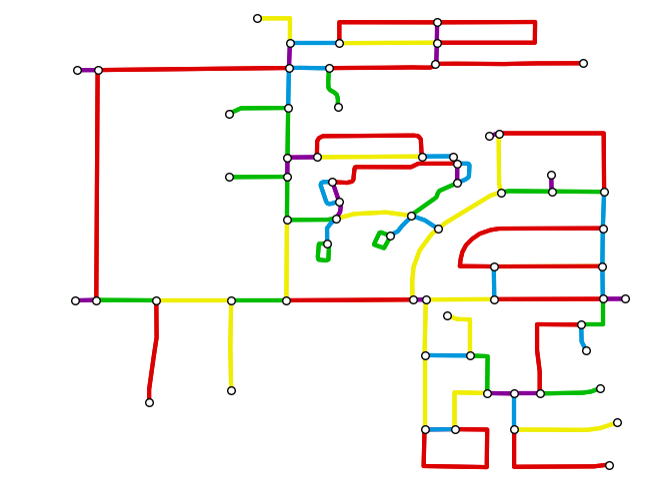
\includegraphics[width=0.4\textwidth]{figures/road-network.png} &
				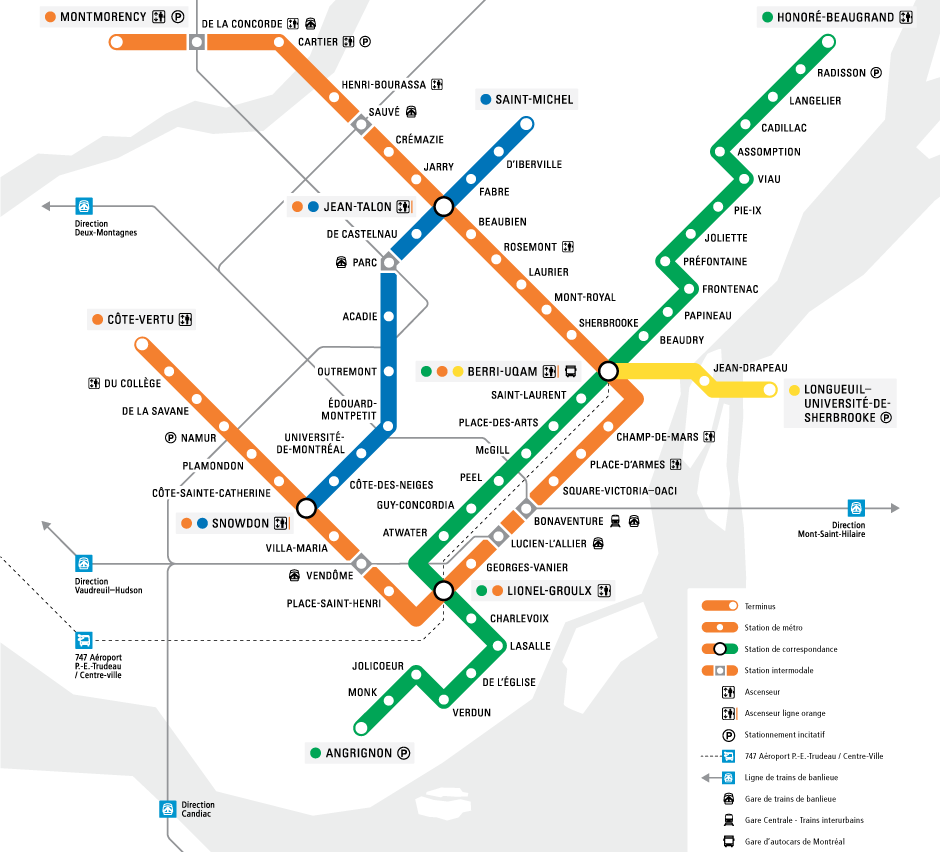
\includegraphics[width=0.4\textwidth]{figures/mtl-metro-cut.png} \\
			\end{tabular}
		\end{center}
		\caption{Example of a typical urban street network (left) and a subway network (right).}
		\caption*{\small Sources: \cite{boeing2017osmnx} (left), \url{http://www.stm.info/fr/infos/reseaux/metro} (right)}
		\label{fig:networks}
	\end{figure*}
	
	Regardless of the working context, we will work with a \textit{network} model, which tends to be quite simple in urban street networks, merely consisting of a directed graph with street segments as nodes, where connection to other street segments indicate that direct navigation is possible. For public transportation networks, as mentioned above, it could be pertinent to consider a more rich representation than a graph of stops and lines, but considering also the routes formed by transportation vehicles, such as buses or trains, visiting stops at set times and allowing commuters to board or alight at them. A well-known model that includes these network elements, among others less interesting for our problem, is \gls{gtfs}\footnote{\url{https://developers.google.com/transit/gtfs/}}, which is widely adopted by open data platforms in numerous Smart Cities.
	
	For any kind of network, a \textit{trajectory} will be defined as a path formed by a sequence of network elements (usually stops or street segments), that was traversed by a single commuter in one trip, with an origin and a final destination. In this definition, we must consider some practical limitations to the nature of a trajectory, as one could argue whether commuters that take more than one hour to switch a line are actually switching or just finalized their trajectories and are starting second ones with some new destination. These cases are complicated to unambiguously decide in practice, and therefore our approach will tend to set hard limits on waiting times and walking distances for a single trajectory.
	
	Our definitions also require to be able to speak for a concept of time. When we work with a public transportation network model integrating routes formed by transport vehicles that follow lines, there would be no need in representing the exact time at which each user has boarded on a stop, only a route identifier, as the stopping times would be already available in our modelled network, this avoiding some redundancy in the representation of trajectories.
	Alternatively, for urban street networks or other cases where route information is unavailable, a representation of time intervals may be considered in order to achieve a compact representation, where time would be expressed in discrete intervals of one to thirty minutes.
	
	Massive data collection techniques exist for both of the network contexts discussed above, as will be later seen in Section~\ref{sec:dm}, leading to the problem of efficiently handling this vast information. Apart from the usual well-known \textit{Big Data} solutions, there is an ongoing research on the application of data structures for some of these goals. In particular, it is possible to apply many of the techniques from the field of \textit{Compact Data Structures} to build autoindexed representations that support efficient query patterns tailored for specific information needs, while offering some sort of compression with respect of a more traditional representation.
	
	A usable solution would also require a user interface that enables the exploitation of this information by researchers, transportation companies, city administrations and any other kind of end users. This interface must, at the very least, allow visualizing the network elements on a map, also granting the ability to make queries over these elements in an intuitive and responsive way, while respecting the usual quality principles of any user-oriented software of this kind.
	
	\section{Contributions}
	As the two contexts from Section~\ref{sec:pd}~lead to different ways of structuring and querying the information, it is natural to expect at least two different representations, one for each context. For this reason, in this work we have applied compact data structures and techniques to design novel representations that are able to handle massive collections of data related to user transportation habits. Our proposed representation cover both contexts, as well as offer a fair trade-off for different query needs, while at the same time ensuring that our proposals can be implemented in a real world scenario, for which we evaluate the performance of our representations with realistic query cases over real datasets\footnote{When needed, the real data was augmented or mixed with synthetic information}.
	
	Furthermore, as a proof of the practicability of our approach, we have developed a user interface that is based on our representations, and allows a user to perform queries through a \gls{gis} web interface. Unlike traditional \gls{gis} interfaces, ours is focused on offering convenient methods to query past user trajectories by network elements instead of purely spatial relationships, and achieves far superior performance when compared to systems backed by traditional database systems.
	
	In conclusion, we present an end-to-end platform around representations based on compact data structures to process, store, query and visualize mined public transportation usage data. To our knowledge, this is the first work to accomplish building such integrated platform, although other works exist that contemplate the use of compact data structures for trajectories or moving objects (see Section~\ref{sec:ti}).
	
	\section{Outline}
	The rest of this thesis is structured as follows: In the following Chapter~\ref{ch:state} we review the literature on existing methods for trajectory extraction and indexing. The former is interesting to our work as it studies different approaches to obtain the trajectories over public transportation systems, which our work focuses on, while the later discusses alternatives for some of the traditional queries over trajectories, that are often based on secondary memory.
	
	After that, our contributions are grouped into two parts:
	
	\begin{itemize}
	    \item In the \textbf{Part~\ref{part:cds}} we propose several representations based on compact data structures to efficiently handle the analysis of trips for both transportation contexts from the Section~\ref{sec:pd}. It is therefore divided in three chapters:
	    
	    \begin{itemize}
	        \item In the Chapter~\ref{ch:cds:prev} we describe the underlying structures that are used by our representations, with a brief description of the memory requirements of each one of them, as well as the temporal complexities of their main algorithms.
	        
	        \item The Chapter~\ref{sec:ctr} is dedicated to our representation for trips in the context of urban street networks. We use separate structures for the spatial and temporal representations, and combine them so that they can be used to solve spatio-temporal queries.
	        
	        \item In the Chapter~\ref{sec:newctr} we discuss the problems specific for trips over public transportation networks, and provide two alternative representations based on a common model, along with an additional complimentary structure that can be used to accelerate some of the aggregation queries.
	    \end{itemize}
	    
	    \item In the \textbf{Part~\ref{part:gis}} we present an interface designed to aid on the decision making process of a public transport agency, that relies on the representations from Part~\ref{part:cds}. This part consists of two chapters:
	    
	    \begin{itemize}
	        \item The Chapter~\ref{ch:gis:prev} serves the role of introducing the reader to some of the basic concepts of \gls{gis}, as well as the technologies used in our developed interface.
	        
	        \item The Chapter~\ref{sec:gis} contains the detailed description of our interface, discussing its architecture and our user interface to analyze historical information of user trips.
	    \end{itemize}
	\end{itemize}
	
	Finally, the \textbf{Part~\ref{part:final}} summarizes our contributions in one single conclusion Chapter~\ref{ch:concl}, where we also discuss the future developments planned for the work exposed in this thesis.
	
\chapter{State of the art in trajectory extraction and representation}
\label{ch:state}
    This chapter is dedicated to provide a context to our contributions with a literature review of tangential works. We start by discussing methods of collecting useful trajectory data, followed by a review of mobile objects and models for the trajectories they generate, as well as types of queries that are often found in mobile objects research. Finally, we look into the most relevant works in trajectory indexing, which contrast with our contributions as the later are based on auto-indexed representations, and are focused on problems specific to the study of transportation demand and travel patterns on transportation networks.

	\section{Trajectory extraction}
	\label{sec:dm}
	In order to make significant conclusions about the travel patterns, it is essential to be able to collect a large enough collection of trips to be representative enough of the overall usage within a time span. For this problem, crowd-sourcing can be a viable approach to record the trajectories of public transportation users, as done in \cite{zimmerman2011field}, where the users were rewarded with real information on the bus location, estimation of arrival time and fullness in exchange of recording the GPS trace on their own bus trips.
	
	Currently there are several known techniques that would allow to collect data regarding users' trips over a public transportation network. Numerous works exist where those trajectories are mined from the transactions of smart cards \cite{bhaskar2015passenger,wang2014aggregated}. This can be complemented with information derived from GPS devices, as shown in \cite{ma2014development}. Alternatively, reliable trajectories may be extracted relying on positioning obtained from cellular networks, as proven by \cite{liu2017exploring}.

    Because smart card methods usually provide only information about boarding stops, there are works that study the challenge of inferring alighting stops from passengers \cite{wang2011review}. In addition, the authors of \cite{tao2014exploring} have specifically tackled the challenge of reconstructing full trajectories, accounting for trip-chaining, by using data obtained from smart cards. Furthermore, in \cite{alsger2016validating} it is also proven that not only the alighting stops, but also the (last) destination stop of a trip can be estimated from boarding data gathered by a smart card, within a reasonable accuracy, given that a transportation network user typically makes a return trip at another time of the day, as happens often with people that commute from their homes to work and back. We find these methods particularly interesting, as a significant portion of the query patterns we propose in order to analyze passenger movements rely on knowing about line switches (trip-chaining) and the ultimate destination of a trajectory.
    
    However, there is little research on methods for exploitation of this extracted information, in order to analyze and improve the efficiency of a transportation network, which constitutes the scope of our work. This summarized review proves that, although we were not able to access real data from a public transportation company for this work, such curated information about users' trips can indeed be obtained and used for our proposed representations.
	
	\section{Models of trajectory and types of queries}
    A good place to begin searching for practical models of trajectory representation is the vast amount of work on designing data models for moving objects~\cite{DBLP:conf/ssdbm/WolfsonXCJ98,DBLP:conf/icde/SistlaWCD97,DBLP:journals/tods/GutingBEJLSV00,DBLP:conf/chorochronos/GutingBEJLNSV03,DBLP:journals/geoinformatica/Spaccapietra01,DBLP:conf/sigmod/ForlizziGNS00,DBLP:journals/geoinformatica/ErwigGSV99,DBLP:books/mk/GutingS2005}. Basically, a moving object data model represents the continuous change of the location of an object over time, this way defining a trajectory.
    
    The moving objects can be seen as a big data problem, where solutions may typically differ in the representation of location, contextual or environmental information where the movement takes place, the time dimension, which can be continuous or discrete, and the level of abstraction or granularity on which the trajectories are described~\cite{DBLP:journals/sigspatial/DamianiIGV15}. A common classification of trajectories distinguishes free from network-based trajectories.  \textit{Free trajectories} or Euclidean trajectories are a sequence of GPS points represented by an ad-hoc data type of moving points~\cite{DBLP:conf/ssdbm/WolfsonXCJ98,DBLP:conf/icde/SistlaWCD97,DBLP:journals/tods/GutingBEJLSV00}. \textit{Network constrained} trajectories are a temporal ordered sequence of locations on networks. This trajectory model includes a data type for representing  networks and  for representing the relative location of static and moving  points on the network~\cite{DBLP:journals/vldb/GutingAD06}. When we want to represent trajectories over an urban street network, it is often useful to deal with \textit{network-matched trajectories}, as this will allow to represent large collections trajectories more efficiently. The process of obtaining these network-matched trajectories from GPS points is called \textit{map-matching} \cite{brakatsoulas2005map}. This process can also be done online, as recently shown in~\cite{DBLP:journals/tits/Ding0GL15}, where all the processing is done in the server, eliminating the need of any map or network representation at the moving object side.
    
    The definition of trajectories at an abstract level must be materialized in an internal representation with access methods for query processing. An early and broad classification of spatial-temporal queries for \textit{historical positions} of moving objects \cite{DBLP:conf/vldb/PfoserJT00} identifies coordinate- and trajectory-based queries. Coordinate-based queries include the well-known  {\it time-slice}, {\it time-interval} and \textit{nearest-neighbor queries}. Examples are \textit{find objects or trajectories in a region at a  particular time instant or during some time interval}. Another important example of coordinate-based queries is \textit{find the k-closest objects with respect to a given point at a given time instant}. Trajectory-based queries  involve topology of trajectories (e.g., overlap and disjoint) and information (e.g., speed, area, and heading) that can be derived from the combination of time and space. An example of such queries would be  \textit{find objects or trajectories that satisfy a spatial predicate (eg., leave or enter a region)  at a particular time instant or time interval}. There also exist combined queries addressing information of particular objects: \textit{Where was object X at a particular time instant or time interval}. In all previous queries, the results are individual trajectories that satisfy the query constraints.
    
    %When dealing with large datasets of trajectories, and due to privacy issues, the individual trajectory cannot be revealed, then anonymized and aggregated trajectories are of concern.  
    In many applications, aggregated trajectories must be analyzed in the collection, as an individual trajectory does not represent any useful information.
    In this context, we can  further distinguish range- from trajectory-based queries. Range queries impose constraints in terms of a spatial location  and temporal interval.  Examples of these queries are  to retrieve the number of distinct trajectories  that intersect a spatial region or spatial location (stop) at a given time instant or time interval, retrieve the number of distinct trajectories that start at a particular location (stop) or in a region and/or end in another particular location of region, retrieve the number of trajectories that follow a path, 
     and retrieve the  top-k locations (stops) or regions  with the larger number of  trajectories that  intersect  at a given time instant or time interval. Trajectory-based queries require not only to use the spatio-temporal points of trajectories  but also the sequence of these points. Examples of such queries are  to find the number of trajectories that are heading (not necessarily ending at) to a spatial location during a time interval, find the destination of trajectories that are passing through a region during a time interval, find the number of starting locations of  trajectories that go or pass through a region during a time interval.
	
	\section{Trajectory indexing}
	\label{sec:ti}
	Literature on spatial trajectory indexing can be categorized by the nature of the trajectories: they can be either constrained to a network or in free space (often called moving objects). While there are well-known queries for indexes that work on moving objects in free space \cite{DBLP:conf/vldb/PfoserJT00}, the network constrained trajectory indexes cover more diverse querying needs, as different networks involve different kinds of challenges (as in vehicular road network vs public transportation network), and also because the intended application may vary (analyzing trip-chaining patterns vs number of passengers within a time window). A comprehensive review on indexing methods can be found in \cite[Chapter 4]{DBLP:books/sp/PelekisT14}, to which we shall expand in the rest of this section to mention the most notable indexes and some new developments.
	
	\subsection{Free trajectory indexing}
	Several adaptations of the {\em R-Tree} \cite{DBLP:conf/sigmod/Guttman84} are widely used for the indexing of moving objects. The most common approach is to integrate the temporal dimension in the R-Tree itself, as found in the {\em STR-Tree} and the {\em TB-Tree} from \cite{DBLP:conf/vldb/PfoserJT00}.
    Another common approach is to compliment the R-Tree with another similar structure, as has been done for the {\em MV3R-tree}~\cite{DBLP:conf/vldb/PapadiasT01},
    where an Historical {\em R-Tree}~\cite{nascimento1998towards} to partition on the temporal dimension.
    
    Generally, even for very large collections of trajectories, the spatial dimensions are more bounded than the temporal dimension, which can grow indefinitely. For this reason, even for free trajectories, temporal dimension is generally more selective than spatial dimensions. This observation was heavily exploited in the subsequent works, such as {\em SETI} from \cite{chakka2003indexing}, where the space is partitioned statically, while trajectories are indexed by their temporal dimension using a one dimensional R-Tree, allowing it to grow dynamically.
    
    Recently a framework based on Apache Spark was developed called {\em UlTraMan}~ \cite{ding2018ultraman}, that supports different kinds of partitioning schemes for large collections of trajectories to answer range, kNN or aggregation queries, allowing to repartition the dataset to maximize the query time efficiency for a given query type. Although UlTraMan has been tested over network constrained trajectories, it does not appear to be exploiting network information in any way, hence its inclusion in this category.
    
    In the field of compact data structures, an index called {\em GraCT}~\cite{brisaboa2019gract} has been developed, based snapshots at regular time intervals using {\em k$^2$-Trees}~\cite{brisaboa2009k} and movement logs for individual trajectories to which grammar compression is applied with {\em RePair}~\cite{larsson2000off}. Because of this, GraCT is a self-indexed compact representation that supports spatio-temporal range and nearest-neighbor queries, as well as allowing for direct access to the trajectory information.
	
	\subsection{Network constrained trajectory indexing}
	There are also numerous approaches that use R-Tree based indexes for trajectories that are constrained to an underlying network, aiming to decrease the redundancy in the representation by separating the representation into levels. Examples of such indexes include the {\em FNR-Tree}~\cite{DBLP:conf/ssd/Frentzos03}, where the network elements are indexed with a 2D R-Tree and 1D R-Trees to index time intervals of moving objects along the edges of the network. Some of the limitations of the FNR-Tree are addressed in \cite{DBLP:journals/geoinformatica/AlmeidaG05}, where the authors propose the {\em MON-Tree}, where the moving objects are indexes in two dimensional R-Trees (the dimensions being edge position vs time). More recent alternatives, such as the {\em TMN-Tree}~\cite{chang2010tmn}, integrate {\em B$^+$-Trees}, which have proven to be more space and time efficient for indexing the temporal dimension. Alternatively, in \cite{rivera2018faster} a compact representation of time intervals is proposed using two bitvectors, that can be combined with these R-Tree based indexes to increase the efficiency for temporal filtering. Refer to \cite{john2017performance} for a quick comparison of these R-Tree based indexes.

    As a competitive alternative to these R-Tree based indexes, {\em PARINET}~\cite{DBLP:journals/vldb/PopaZOBV11}, builds spatial partitions from the trajectories based on their distribution and network topology, and uses a B$^+$-Tree to index the trajectories in each partition by time intervals. Although candidate trajectories must be filtered in memory during queries, PARINET is highly efficient in practice as its partitioning strategy minimizes the number of disk accesses needed.
    %The same ideas were used in {\em TRIFL}~\cite{that2015trifl}, where the cost model is adapted for flash storage.
    
    Another relevant representation is described in \cite{DBLP:conf/gis/KroghPTT14}. Their proposed index, {\em NETTRA}, was designed to efficiently solve a specific kind of query called {\em Strict Path Queries (SPQ)}, built on a traditional RDBMS with $B^+$-Tree indexes. Another distinctive feature of NETTRA is its treatment of network constrained trajectories as textual information, which allows to apply string matching techniques such as fingerprinting functions to determine what trajectories have similar paths on their traversed edges. This close equivalence between trajectories and strings has been further exploited by Geodabs~\cite{chapuis2018geodabs}, where both the spatial distribution and sequence information are taken into account for finding trajectories by similarity with fingerprinting. These text-based approaches are sometimes tangled with works on the topic of semantic trajectories such as \cite{al2017semantictraj}.
    
    %For vehicles we also have this \cite{cai2018vector} and \cite{lovell2018lossless}.
    
    A recent compact data structure named {\em CiNCT} has been proposed in \cite{koide2018cinct}, where trajectories are encoded into a string, that is used to build an FM-index \cite{DBLP:conf/focs/FerraginaM00} with a Huffman-shaped Wavelet Tree \cite{ferragina2009compressed}. To further save space, the string is constructed with relative movement labels instead of absolute edges, with an auxiliary structure that represents a network graph built from the input trajectories themselves. While this structure excels at pattern-matching and path extraction in vehicular networks (such as the streets of a city), it cannot be applied to our problems in public transportation networks, where network demand and aggregated travel patterns have to be analyzed, while finding out which trajectories traversed on a specific path of sequential street segments does not, in itself, provide us much relevant information.
	
	
\part{Compact representation of trajectories over transportation networks} \label{part:cds}
\chapter{Previous concepts}
\label{ch:cds:prev}
	This chapter may serve as an introduction to the compact data structures used in our proposed representations, and it should give a sufficient understanding of the underlying concepts that we will be working with for the rest of this part. For a more in-depth guide on compact data structures, the reader may refer to \cite{Nav16}.
	%, where they are introduced from basic information theory concepts such as entropy.
	
	A reader who is already familiar with compact data structures is still encouraged to read the Section~\ref{sec:sat}, where the \gls{sat} is introduced, which is initially unrelated to compact data structures, and also the Section~\ref{sec:wt}, where we discuss some less known variants and operations of the \gls{wt}, that we make use of in our contributions.
	
	\section{Summed Area Table}
	\label{sec:sat}
	The \gls{sat} was first introduced in computer graphics \cite{crow1984summed} to speed up the mipmapping process, where given a texture image represented as bidimensional matrices of numbers (usually three matrices of integers, one for each color channel) we are interested in finding the average color of any arbitrary rectangle within the image. This operation is most often used to reduce the rendering time for distant polygons where a pixel on the target screen may correspond to several texture pixels (texels), and also for anisotropic filtering, in order to improve the visual quality of polygons that are projected in an oblique angle.

    With the most direct representation of a matrix as an array of values, we are required to compute the average value of a rectangle $(a,b),(a+h,b+w)$ as:
    
    \[
    \overline{M}_{a..a+h,b..b+w}~\leftarrow~
    \frac{\displaystyle\sum^h_{i=0}\displaystyle\sum^w_{j=0}M_{i+a,j+b}}
    {(h+1)(w+1)}
    \]
    
    Note that the summation has a time complexity of $O(hw)$, which would make this operation quite expensive for real time rendering applications. In order to improve the complexity of these calculations, the \gls{sat} precomputes the summations of $M$ in a matrix $I$, of the same size, where $I_{a,b}~\leftarrow~\displaystyle\sum^a_{i=0}\displaystyle\sum^b_{j=0}M_{i,j}$. That is, each cell of $I$ is the sum of the values within rectangle spanning from the origin of the matrix to the position of the cell. An example of a \gls{sat} can be found in the Figure~\ref{fig:sat}.
    
    \begin{figure}[ht]
		\begin{center}
			{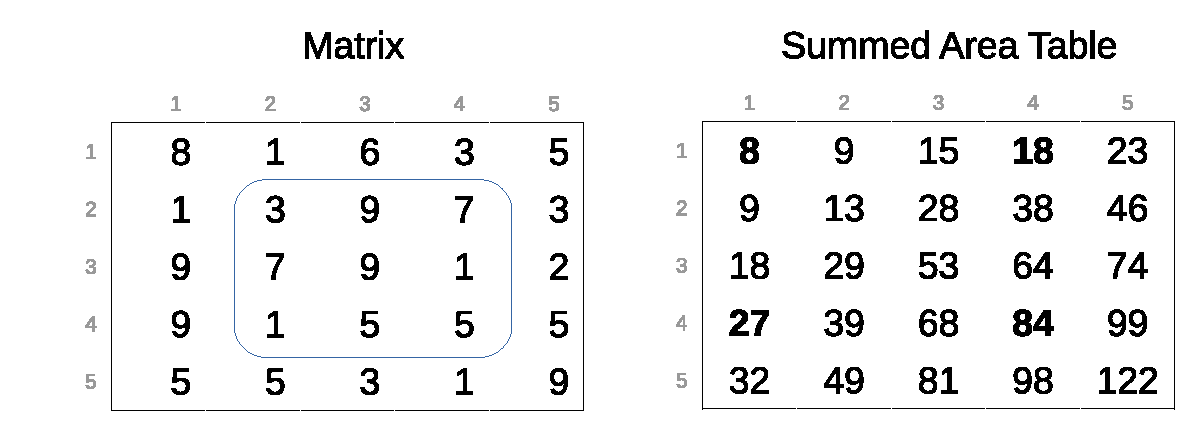
\includegraphics[width=0.8\textwidth]{figures/example_sat.eps}}
		\end{center}
		\caption{An example of a \acrlong{sat} (right) built over a matrix (left).}
		\label{fig:sat}
	\end{figure}
    
    Having $I$, we can compute the average value of a rectangle in $O(1)$ operations as:
    
    \[
    \overline{M}_{a..a+h,b..b+w}~\leftarrow~
    \frac{I_{a+h,b+w} - I_{a+h,b-1} - I_{a-1,b+w} + I_{a-1,b-1}}
    {(h+1)(w+1)}
    \]
    
    In our example from Figure~\ref{fig:sat}, to calculate the sum of the delimited $3x3$ region in the matrix, we simply operate over the four terms in \textbf{bold} from the \gls{sat}, obtaining
    $\displaystyle\sum^4_{i=2}\displaystyle\sum^4_{j=2}M_{i,j}~=~I_{4,4}-I_{4,1}-I_{1,4}+I_{1,1}~=~84-27-18+8~=~47$.
    
    While with this representation we do not need to keep the original matrix\footnote{As accessing a single cell can be viewed as a special case of the computation of an average where $h=0,w=0$.}, the improved computational efficiency comes at the expense of having to represent larger numbers than the original values.
	
	\section{Entropy coding}
	Given an information source (such as a text) that provides symbols from an alphabet $[1..\sigma]$ with a probability of $0 \leq p_i \leq 1$ for each symbol, where $\displaystyle\sum_ip_i=1$, the goal of an entropy coder is to exploit these probabilities in order to achieve compression by assigning shorter codes to the most frequent symbols, and longer to the less frequent ones. In the work that is considered as the foundation of information theory \cite{shannon1948mathematical}, Claude Shannon defined a concept called \textit{entropy}, which is closely related to the probabilities we are discussing, and used it to prove that the when encoding the symbols in binary, the optimal length in bits for each code is of $l_i = \frac{1}{\log_2p_i} = -\log_2p_i$ bits, and the entropy of an information source $S$ calculated as $H_0(S) = -\displaystyle\sum^\sigma_i p_il_i = -\displaystyle\sum^\sigma_i p_i\log_2p_i$.
	
	As this compression technique relies on using variable-length codes, it is necessary that the codes are unambiguous: there can be no two codes $C_i, C_j$ that, when concatenated, can be interpreted as another code 
	% esto esta mal porque no contempla el caso de concatenar tres o mas codigos ambiguos
	%($C_iC_j \neq C_k, \forall i,j,k \in [1..\sigma]$)
	. Additionally, it is computationally very useful for those codes to also be prefix-free, meaning that there can be no code that is the prefix part of another ($C_i \neq C_j0^a1^b,~\forall i,j \in [1..\sigma], i\neq j, a,b \in [0..\infty)$), as this will allow us to unambiguously interpret the symbol right after the bits of $C_i$ are read, without having to determine if it could be the prefix part of some other longer code $C_j$.
	
	The Huffman coding, introduced in \cite{huffman1952method}, is a coding algorithm that produces prefix-free and optimal\footnote{That is, with lengths as close to $-\log_2p_i$ as possible with a whole number of bits per symbol.} codes based on the frequencies of each symbol. The ideas of the Huffman coding have been widely implemented in numerous compression algorithms and codecs since its inception, where the most notable examples are DEFLATE (PKZIP, GZIP), JPEG and MPEG.
	
	One less known variation of the Huffman codes are the Hu-Tucker codes \cite{hu1971optimal}, which aim to provide codes that preserve the same lexical order as the original symbols, meaning that for any two symbols $s_i,s_j$, it holds that $s_i \prec s_j \iff C_i \prec C_j$. This comes at the expense of at most one extra bit per code over Huffman on average\footnote{Being $L_h$ and $L_{ht}$ the average codeword 
	length of Huffman coding and Hu-Tucker codes for $S$ respectively, it holds: $H_0(S) \leq L_h \leq H_0(S)+1$ and $H_0(S) \leq L_{ht} \leq H_0+2(S)$
	(see \cite{Cover:2006:EIT:1146355} (pages 122-123), or \cite{HORIBE1977148, GilbertandMore1959}).}.
	
	\section{Bitvectors}
	\label{sec:bit}
	A great amount of works in compact data structures involves the use of bitvectors, both compressed and uncompressed. A bitvector $B[1..n]$ is a sequence of $n$ bits, for which the following operations are expected to be supported:

    \begin{itemize}
        \item $\rank_1(B,i)$ is the number of set bits in $B[1..i]$. Alternatively, $\rank_0(B,i)~\leftarrow~i - \rank_1(B,i)$. Consequently, it also holds that the bit from the position $i$ can be retrieved as $B[i] = \rank_1(B,i) - \rank_1(B,i-1)$.
        \item $\select_1(B,i)$ is the position in $[1..n]$ where the $i$th 1 occurs. Therefore, $\rank_1(B,\select_1(B,i)) = i$. An equivalent version for 0 bits may be defined as $\select_1(B,i)$, although, unlike with $\rank_0$, there does not exist a direct way of obtaining it from the previously defined operations.
    \end{itemize}
    
    \begin{example}
        Given a bitvector $B = 011001$, it holds that $\rank_1(B,1) = 0$, $\rank_1(B,2) = 1$, $\rank_1(B,3) = 2, \rank_1(B,4) = 2$. Furthermore, $B[3] = \rank_1(B,3) - \rank_1(B,2) = 1$ and $\rank_0(B,3) = 3 - \rank_1(B,3) = 1$.
        
        We can also say that $\select_1(B,2) = 3$ and $\select_1(B,3) = 6$, thus holding that $\rank_1(B,\select_1(B,2)) = \rank_1(B,3) = 2$ and $\rank_1(B,\select_1(B,3)) = \rank_1(B,6) = 3$. Additionally, $\select_0(B,2) = 4$ as $\rank_0(B,\select_0(B,2)) = \rank_0(B,4) = 2$.
        \qed
    \end{example}
    
    All these operations can be supported in $O(1)$ time with $o(n)$ extra bits \cite{Jac89,Mun96}. 
    Additionally, there exist several techniques for compressing these bitvectors based on their arrangement although several techniques exist for compressing bitvectors depending on their statistical properties. In this work we will use a representation that excels in efficiently solving $\select_1$ operations for sparse bitvectors (with a low number of set bits in proportion to the bitvector size) introduced in \cite{okanohara2007practical}, and also another representation that works particularly well with non uniformly distributed bitvectors, thus exploiting their entropy to require only $nH_0(B) + o(n)$ bits\footnote{Being $n_1$ the number of set bits in $B$ and $n_0 = n - n_1$, then $H_0(B) = \dfrac{n_1\log\dfrac{n}{n_1} + n_0\log\dfrac{n}{n_0}}{n} \leq 1$.} \cite{Raman:2002:SID:545381.545411}.
	
	\section{Wavelet Tree and Wavelet Matrix}
	\label{sec:wt}
	When working with a sequence $S[1..n]$ over an alphabet $[1..\sigma]$, we can extend the definitions of $\rank$ and $\select$ from the Section~\ref{sec:bit} to work over an any symbol $a \in [1..\sigma]$ instead of bits, resulting in the following operations:
	
	\begin{itemize}
	    \item $\rank_a(S,i)$ is the number of occurrences of the symbol $a$ in $S[1..i]$.
	    \item $\select_a(S,i)$ is the position in $[1..n]$ where the $i$th $a$ occurs.
	\end{itemize}
	
    The \gls{wt} \cite{WT03} represents $S$ with a balanced binary tree, with $\sigma$ leaves, one for each symbol. Every internal node $v$ represents a the range of symbols $[\alpha_v..\omega_v] \subseteq [1..\sigma]$ in the same order as they appear in $S$, where the root node corresponds to all the $n$ symbols from the alphabet $[1..\sigma]$ appearing in $S$. Its left child $v_l$ will only represent the $n_l$ symbols that fall in the range $[1..\dfrac{\sigma}{2})$, preserving the order that they had in $v_0$, while the right child will represent the other $n_r$ symbols from $[\dfrac{\sigma}{2}..\sigma]$, holding that $n_l+n_r=n$. This is built recursively until a leaf $v_a$ is reached, with will correspond to only one symbol $a \in [1..\sigma]$, with $n_a = \rank_a(S,n)$ times. An example \gls{wt} can be found in Figure~\ref{fig:wt}.
    
    \begin{figure}[ht]
		\begin{center}
			{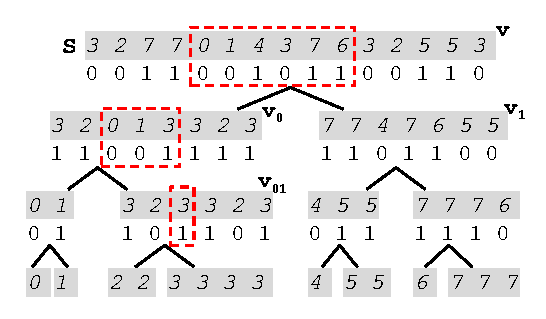
\includegraphics[width=0.65\textwidth]{figures/wt1.eps}}
		\end{center}
		\caption{An example \acrlong{wt} of four levels.}
		\label{fig:wt}
	\end{figure}
    
    For each node $v$, these symbols from the alphabet $[\alpha_v..\omega_v]$ are represented implicitly using a bitvector $B_v[1..n_v]$, where $B[i] = 0$ when the symbol $a$ represented in the position $i$ should belong to the left child ($a < \dfrac{\alpha_v + \omega_v}{2}$), while $B[i] = 1$ means it should belong to the right child ($a \geq \dfrac{\alpha_v + \omega_v}{2}$). By making use of $\rank$ and $\select$ operations over these bitvectors, we are able to recover the value of any $S[i]$, and also answer $\rank_a$ and $\select_a$ for any $a \in [1..\sigma]$ in $O(\log\sigma)$ without the need of storing the original sequence. As there are $n$ bits per level and $\log\sigma$ internal levels (the nodes from the leaf level do not have bitvectors), we could represent every bitvector in $n\log\sigma$ bits, which is equivalent to the space it would take to represent $S$ as an array of fixed length integers\footnote{When $\sigma$ is not a power of two, $\log\sigma$ would need to be rounded up for fixed length integers, while for the \gls{wt} there will be some leaves at level $h-1$, being $h$ the height of the tree, and its total size will depend on the frequency of those symbols ($\lfloor n\log\sigma\rfloor < \sum_i n_i < \rceil n\log\sigma\rceil$.}). However, we also need some auxiliary structures for $\rank_1$ and $\select_1$, which will require $o(n\log\sigma)$ bits and also store a pointer for every one of the $2\sigma-1$ nodes. Therefore, the total size of this representation amounts to $n\log\sigma + o(n\log\sigma) + O(\sigma\log n)$.
    
    In order to access the value of $S[i]$, we must start by looking into $B_v[i]$ from the root node. If $B_v[i]=0$, we traverse to the position $B_{v_0}[\rank_0(B_v,i)]$ of the bitvector of the left child. Conversely, when $B_v[i]=1$, we traverse to the bitvector of the right child at $B_{v_1}[\rank_1(B_v,i)]$. In both cases, we recurse until a leaf is reached, which will unambiguously correspond to a symbol $a$, thus we determine that $B_v[i]=a$.
    
    \begin{example} \label{exp:wtaccess}
    In the \gls{wt} from Figure~\ref{fig:wt}, if we wanted to retrieve the value of $S[2]$, we would start by looking into the bit $B_v[2]=0$, meaning that the we have to traverse to the node $v_0$ and look into the bit $B_{v_0}[\rank_0(B_v,2)] = B_{v_0}[2] = 1$, leading us to the node $v_{01}$ at $B_{v_{01}}[\rank_1(B_{v_0},2)] = B_{v_{01}}[2] = 0$. The left node is a leaf node belonging to the symbol $2$, so $S[2]=2$ (namely, the first occurrence of $2$ in $S$, as $\rank_0(B_{v_{01}}, 2) = 1$).
    \qed
    \end{example}
    
    We can also solve $\rank_a$ by traversing the tree from top to bottom with the bitvector $\rank$ operation: knowing that the binary representation (and thus also the path in the \gls{wt}) of a symbol will allow us to use $\rank_1$ or $\rank_0$ in each level $i$ according to the $i$th bit of our code. In the Example~\ref{exp:wtaccess}, knowing that the binary representation of $2$ is $010$, we can calculate $\rank_2(S,2)$ (or any other position) following the same order of operations: a $\rank_0$, a $\rank_1$ and one final $\rank_0$ to determine the position of the leaf node, which will give away $\rank_2$. It is also possible to calculate $\select_a(S,i)$ with a bottom to top traversal of the tree, by starting at the $i$th position from the leaf belonging to $a$, and applying $\select_0$ and $\select_1$ on the bitvectors of the parent nodes, following the reversed binary code of $a$. Eventually, a position $S[i]=a$ will be reached such that it will contain the $i$th occurrence of $a$ in $S$.
    
    A more complex operation that we have found very useful in our work in is the $\cnt_{a,b}(S,i,j)$, first described in \cite{gagie2012new}, which counts the number of occurrences of symbols in $[a..b]$ within $S[i..j]$. While it is equivalent to $\displaystyle\sum^b_{k=a}\rank_k(S,j) - \rank_k(S,i)$, it can be solved more efficiently by doing two simultaneous top to bottom traversals, as described for $\rank_a$. Starting at the root node $v$ we calculate $\rank_0(B_v,i)$ and $\rank_0(B_v,j)$ to find out the limits in the left node for the codes within $[a..b]$ that start with 0, and also $\rank_1(B_v,i)$ and $\rank_1(B_v,j)$ for those codes starting by 1. If all of the codes in $[a..b]$ start with either a zero or a one, we will only compute the corresponding $\rank$. After that, we recurse for each node, where on the left $i~\leftarrow~\rank_0(B_v,i)$, $j~\leftarrow~\rank_0(B_v,j)$ and we only consider the range of symbols $[a..b']$ that can be represented by that node ($b' \leq \omega_{v_0})$). The same is true for the recursion on the right, where $i~\leftarrow~\rank_1(B_v,i)$, $j~\leftarrow~\rank_1(B_v,j)$ and $\alpha_{v_1} \leq a'$. Therefore, 
    \begin{align*}
    \cnt_{a,b}(v,i,j) = &\cnt_{a,b'}(v_0,\rank_0(B_v,i),\rank_0(B_v,j))\\
    &+~\cnt_{a',b}(v_1,\rank_1(B_v,i),\rank_1(B_v,j))
    \end{align*}
    , recursively. The recursion on each node $v$ stops when $a \leq \alpha_v$ and $\omega_v \leq b$, in which case the count for that node is reported as $j-i+1$. Finally, all the counts are summed and the total amount of occurrences is obtained. While it may look as if the worst case would imply traversing every of the $\sigma$ internal nodes, it is avoided by stopping the recursion when $a \leq \alpha_v$ and $\omega_v \leq b$, thus requiring us to visit only $O(\log\sigma)$ nodes\footnote{In fact, the best case is $cnt_{1,\sigma}(S,i,j) = j-i+1$, which is solved without traversing at all!}. In the \gls{wt} from Figure~\ref{fig:wt}, we have marked the considered ranges for solving $\cnt_{3,3}(S,5,10)$. Additionally, when the subsequence $S[i..j]$ is sorted, we can define $[l..r]~\leftarrow~\cnt^{LR}_{a,b}(S,i,j)$, which returns the upper and lower limits $S[l..r]$ of the occurrences of the symbols $[a..b]$. Naturally, $S[l..r] \subseteq S[i..j]$.
    
    \subsection{Hu-Tucker Wavelet Tree}
    A straightforward way of reducing the size of a \gls{wt} is to use compressed bitvectors, as discussed in \cite{CNspire08.1}, allowing to represent a \gls{wt} in $nH_0(S) + o(n\log\sigma) + O(\sigma\log n)$ bits \cite{WT03}. There is, however, a different approach to achieve similar space requirements is to use a prefix-free variable-length encoding for the symbols.
    For example, Huffman code \cite{huffman1952method} can be used to build a
    Huffman-Shaped \gls{wt} \cite{ferragina2009compressed}, where the tree is not balanced
    anymore, as level of each leaf $v_a$ will be the number of bits for the Huffman code of $a$, which will depend on the frequency of $a$ in $S$. The size reduces to $n(H_0(S)+1)+ o(n(H_0(S)+1)) +  O(\sigma \log n)$\footnote{$O(\sigma \log n)$ term 
    includes both the tree pointers and the size of the Huffman model.}, while average time becomes
    $O(H_0(S))$ for $\rank_a$, and $\select_a$  (the worst-case time is still $O(\log\sigma)$ 
    \cite{Barbay:2013:CPA:2562345.2562626}). By using compressed
    bitvectors \cite{CNspire08.1} space can be even further reduced to $nH_0(S) + o(n(H_0(S)+1)) +  O(\sigma \log n)$.
    Unfortunately, the Huffman codes (including \textit{canonical Huffman}) assigned to
    lexicographically adjacent symbols do not maintain that lexicographic order, and it is not possible to have a $O(\log\sigma)$ bound for $\cnt_{a,b}(S,i,j)$ anymore.
	
	In order to support $\cnt_{a,b}(S,i,j)$ more efficiently, Hu-Tucker codes \cite{hu1971optimal} can be used instead. While the compression achieved by a \gls{htwt} \cite{barbay2009compressed} degreades slightly with respect to using Huffman coding, yielding a bound of $n(H_0(S)+2) + o(n(H_0(S)+1)) +  O(\sigma \log n)$\footnote{This can be reduced to  $nH_0(S) + o(n(H_0(S)+1)) +  O(\sigma \log n)$ by using compressed bitvectors as well.}, the codes for adjacent symbols are lexicographically contiguous. Therefore, we can guarantee a bound of $O(\log\sigma)$ for $\cnt_{a,b}(S,i,j)$ again. An example of a \gls{htwt} in practice can be found in the Figure~\ref{fig:wtwm}.
	
	\subsection{Wavelet Matrix}
	\label{sec:wm}
	For large alphabets, the size of the \gls{wt} is affected by the term $ O(\sigma \log n)$. A {pointerless}
    \gls{wt} \cite{CNspire08.1} permits to remove\footnote{In a pointerless Huffman-shaped \gls{wt}  a
    term $O(\sigma \log\log n)$ still remains due to the need of storing the canonical Huffman model.} 
    that term by concatenating all the bitvectors level-wise 
    and computing the values of the pointers during the \gls{wt} traversals. 
    The operations on a pointerless \gls{wt} have the same time complexity but become slower in practice. 
    
    By reorganizing the nodes in each level of a pointerless \gls{wt}, the \gls{wm} \cite{CNO15} obtains the  same space requirements, yet its performance is very close 
    to that of the regular \gls{wt} with pointers. Figure~\ref{fig:wm} contains an example of a \gls{wm}, representing the same sequence as in Figure~\ref{fig:wt}.
    
    \begin{figure}[ht]
	\begin{center}
		{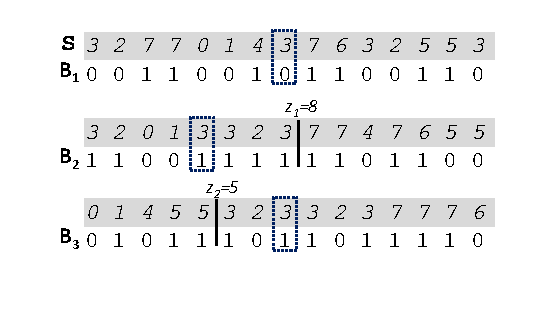
\includegraphics[width=0.65\textwidth]{figures/wm1.eps}}
	\end{center}
	\caption{An example \acrlong{wm} of three levels. A conceptual fourth level was omitted since it does not contain a bitvector.}
	\label{fig:wm}
	\end{figure}
    
    As in the \gls{wt}, the $i$-th level stores the $i$-th bits of the encoded symbols. 
    A single bitvector $B_i$ is kept for each level. In the first level, $B_1$ stores the
    $1$-st bit of the encoding of the symbols in the order of the original sequence $S$.
    From there on, at level $i$, symbols are reordered according to the $(i-1)$-th bit of their encoding; 
    that is, according to the bit they had in the previous level.
    Those symbols whose encoding had a zero at position $i-1$ must be arranged before those that
    had a one. After that, the relative order from the previous level is maintained. That is, if 
    a symbol $a$ occurred before other symbol $b$, and the $(i-1)$-th bit of their encoding
    coincides, then $a$ will precede $b$ at level $i$. %Note that, following this rule,
    %the symbols in the last level shall be ordered by their reversed bit encoding.
    
    If we simply keep track of the number of zeros at each level $z_l\leftarrow \rank_0(B_l,n)$, we can easily see that the symbol with the $k$-th zero
    at level $i-1$ is mapped at position $k$ within $B_i$, whereas the symbol with the $j$-th one at level $i-1$ is 
    mapped at position $z_l +j$ within $B_i$. This avoids the need for pointers, enabling to retain
    the same time complexity of the \gls{wt} operations, including $\cnt_{a,b}(S,i,j)$. For 
    implementation details see \cite{CNO15,ordonez2015statistical}. 
    
    \begin{example}
    To find out the symbol at $S[8]$, we start by observing that $B_1[8]=0$ and $\rank_0(B_1,8)=5$. We move to the next level where we check position $5$; we see that $B_2[5]=1$ and $\rank_1(B_2,5)=3$. We move to next level and check position $3+z_2 = 3+5 = 8$,
    where we finally see $B_3[8]=1$. Therefore, we have decoded the bits $\mathbf{011}$ that correspond to the symbol $S[8] = 3$.
    \qed
    \end{example}
    
    To reduce the space needs of \gls{wm} we could use compressed bitvectors as for \gls{wt}. Yet, 
    compressing the \gls{wm} by giving it either a Huffman or Hu-Tucker shape is not possible as the reordering of the \gls{wm} would lead to the existence of %holes in the structure 
    gaps in the bitvectors 
    that would ruin the process of 
    tracking symbols during traversals. To overcome this issue, an optimal Huffman-based coding was 
    specifically developed for wavelet matrices \cite{CNO15, Farina2016}. This allows to obtain space
    similar to the one a pointerless Huffman-shaped \gls{wt} but with faster $\rank_a$ and $\select_a$ operations.
    Unfortunately, since the encodings of consecutive symbols do not keep the same order, $\cnt_{a,b}(S,i,j)$ is no longer supported in $O(\log\sigma)$ time.
    %and computing $\rank_a(S,j)-rank_c(S,i)+1$ is required for each $c$ in $[\alpha,\beta]$.
	
	\section{Compressed Suffix Array}
	\label{sec:csa}
	Given a sequence $S[1..n]$ built over an alphabet $\Sigma$ of length
    $\sigma$, the {\em suffix array} $A[1..n]$ is built over $S$ \cite{MM93}
    as a permutation of the positions $i \in [1..n]$ of all the suffixes $S[i..n]$, so that
    $S[A[i]..n] \prec S[A[i+1]..n]$ for all $1 \le i < n$
    %, being $\prec$ the lexicographic ordering. 
    Because $A$ contains all the suffixes of $S$ in lexicographic order,
    we can use this structure to search for any pattern $P[1..m] \in S$ in time
    $O(m \log n)$ by simply performing binary searches for the range $A[l..r]$ that
    contains pointers to all the positions in $S$ where $P$ occurs.
    %For the construction of the $A$ a linear time construction
    %algorithm such as the SA-IS~\cite{nong2011two} could be used.
    %which is based on induction sorting.
    We can find an example of an suffix array $A$ in the Figure~\ref{fig:csa}. Any pattern $P[1..m] \in S$ (such as $ana$) can be delimited by a range $A[l..r]$ (for $ana$ it is $A[3..4]$), where the limits $l$ and $r$ can be found with binary searches due to the suffixes being sorted.
    
    \begin{figure}[ht]
		\begin{center}
			{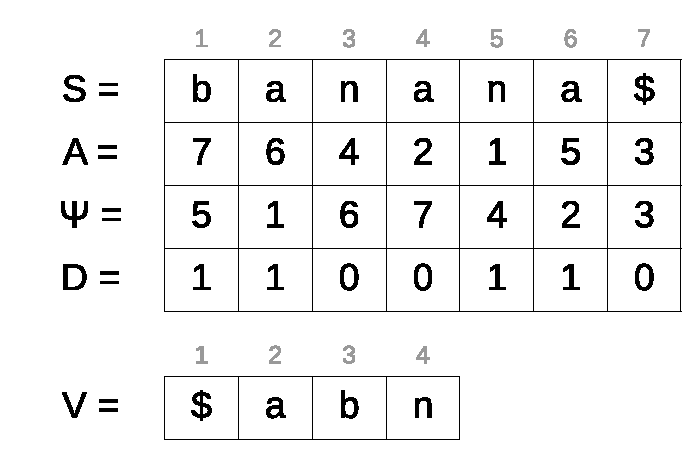
\includegraphics[width=0.5\textwidth]{figures/csa.eps}}
		\end{center}
		\caption{All the structures involved in constructing a \acrlong{csa} over the sequence $S = banana\$$. Note that $S$ and $A$ do not need to be stored.}
		\label{fig:csa}
	\end{figure}
    
    A straightforward enhancement to avoid storing the original string $S$ is to set up a vocabulary array $V[1..\sigma']$, with all the different symbols from $\Sigma$ appearing in $S$\footnote{$\sigma' \leq \sigma)$, since some of the symbols from $\Sigma$ may never appear in $S$.}, and a bitvector $D[1..n]$ aligned to $A$ so that $D[1]=1$ and $D[i]=1~\iff~S[A[i-1]] \neq S[A[i]]$ for all the other $i \in [2..n]$. This means that $D$ marks with a $1$ the beginning of a range of suffixes pointed from $A$ such that the first symbol of those suffixes coincides. With $D$, keeping $S$ is not longer needed since $S[A[i]] = V[\rank_1(D,i)]$.
    
    We also replace $A$ as described in Sadakane's \gls{csa} \cite{Sad03}, using
    another permutation $\Psi[1..n]$ defined in \cite{GV00}, where $\Psi[i] = A^{-1}[A[i]+1]$. That is, for every $A[i]=k$ and $A[j]=k+1$, $\Psi[i]=j$.
    %For each position $j$ in $S$ pointed from $A[i]=j$, $\Psi[i]$ gives the position $z$ such that $A[z]$ points to $j+1$. 
    The special case when $A[i]=n$\footnote{$i=1$ if we use the unique terminator $\$$.} is handled as $\Psi[i]=A^{-1}[1]$, making a cycle.
    Therefore, the \gls{csa} is formed by $\Psi$, $D$, and $V$, which are sufficient to simulate binary searches of the interval $A[l..r]$ for the occurrences of $P$ without the need of accessing $A$ nor $S$. In this work, we define that operation as $[l..r]~\leftarrow~\bsearch(\Psi,P)$.
    The symbol $S[A[i]]$ pointed by $A[i]$ can be obtained as
    $V[\rank_1(D,i)]$. We can also easily obtain the following symbol from the source sequence  $S[A[i]+1]$ as
    $V[\rank_1(D, \Psi[i])]$, $S[A[i]+2]$ can be obtained as $V[\rank_1(D, \Psi[\Psi[i]])]$, and so on.
    %Therefore, the \gls{csa} replaces $S$, and it does not need $A$ anymore to perform searches.
    
    Although an uncompressed $\Psi$ would have the same space requirements
    as $A$, it is highly compressible, since it is formed by $\sigma$ strictly increasing subsequences. By using $\delta$-codes of the gaps (differences of each value with respect to the previous one) we are able to compress $\Psi$ to around the zero-order entropy of $S$~\cite{Sad03}, with $nH_0(S)+O(n\log\log\sigma)$ bits.
    In \cite{NM07} it has been further proved that $\Psi$ can be split into
    at most $nH_k+\sigma^k$ (for any $k$) {\em runs} of consecutive values so
    that the differences within those runs are always $1$. This allows for a combination of $\delta$-coding of gaps with run-length
    encoding (of $1$-$runs$) to achieve a higher-order compression of $\Psi$ without further intervention.
    In addition, to maintain fast random access to $\Psi$, absolute
    samples at regular intervals (every $t_{\Psi}$ entries) are kept. Parameter
    $t_{\Psi}$ implies a space/time trade-off. Larger values lead to better compression of $\Psi$ but slow down access time to non-sampled $\Psi[i]$ values.
    
    In \cite{FBNCPR12}, the authors have adapted Sadakane's \gls{csa} to deal with large (integer-based) alphabets
    and created the {\em integer-based CSA} ($iCSA$). They also showed that, in their scenario (natural language text indexing), the best
    compression of $\Psi$ was obtained by combining differential encoding of runs with Huffman and
    run-length encoding.

\chapter{Representations for trajectories over urban streets}
\label{sec:ctr}
	As explained in Section~\ref{sec:pd}, we have identified two contexts for public transportation systems according to their networks, which can be based on urban streets or public transportation. While the proposed structure in this chapter is capable of operating within both contexts, it does not take public transportation elements (routes and vehicles) into account. This leads to a more redundant representation than the ones later proposed in Chapter~\ref{sec:newctr}, which are more adequate for public transportation networks.
	
	The work in this chapter proposes a new structure named \acrfull{ctr} that answers  counting-based queries and uses compact self-indexed data structures to represent the large amount of trajectories in compact space.
	\gls{ctr} combines two well-known data structures. The first one,
	initially designed for the representation of strings, is the
	\gls{csa}. The second
	one is the \gls{wt}. With these two structures, \gls{ctr} is able to efficiently resolve queries over trajectory patterns in any dimension (spatial, temporal or, combining both structures, spatio-temporal).

    In Section \ref{sec:ctr:desc} we present our scenario, and describe the simplified data model used to represent user trajectories. The most interesting queries that are defined for this scenario are also discussed. Then, Section~\ref{sec:ctr:str} describes the internals of \gls{ctr} and Section~\ref{sec:ctr:alg} is devoted to explain how query operations are solved in \gls{ctr}. After that, experiments are included in Section~\ref{sec:ctr:exp}.

	We experimentally tested our proposal using two sets of %synthetic
	data representing trajectories over two different real public
	transportation systems. Our results are promising because the
	representation uses around  $50$\% of its original size and
	answers most of our spatial, temporal,  and spatio-temporal queries within $1\!-\!1000$ microseconds. 
	No experimental comparisons with classical spatial or spatio-temporal
	index structures were possible, because none of them were designed to
	answer the types of queries in this work. Our approach can  be
	considered as a proof of concept that opens new application
	domains for the use of well-known compact data structures such as the
	\gls{csa} and the \gls{wt}, creating a new strategy for
	exploiting trajectories represented in a self-indexed way.

\section{Description}
\label{sec:ctr:desc}
    Given a transportation network, whether it is based on urban streets or public transportation, we work with a representation of the network that is based on a directed graph. For an urban street network, a \textbf{node} represents a road segment delimited by intersections, where two nodes are connected by an edge if it is possible (i.e. legally allowed). This allows to accurately describe a trajectory by sequentially listing the road segments that were traversed, while minimizing the redundancy.

	%In the other hand, for public transportation networks we define the nodes as stops or stations, making two of them connected if there exists a line or route that stops at each, consecutively. We can represent user trajectories following the same strategy as for urban street networks, although that will lead us to redundant representations in most cases. On subway and bus networks it is common to find stops that belong to only one route, and therefore must be either the end of a trajectory or be followed by the only possible next node. Furthermore, a more minimalist representation of a trajectory with the starting, ending and route switching nodes alone would be sufficient to reconstruct the original trajectory. Such representation will be contemplated later in Chapter~\ref{sec:newctr}, while on \gls{ctr} we maintain a common representation strategy for both kinds of networks. Because listing every node traversed introduces redundancy on public transportation networks, we state that \gls{ctr} is more adequate for urban street networks.
	
	\begin{figure}[ht]
		\begin{center}
			{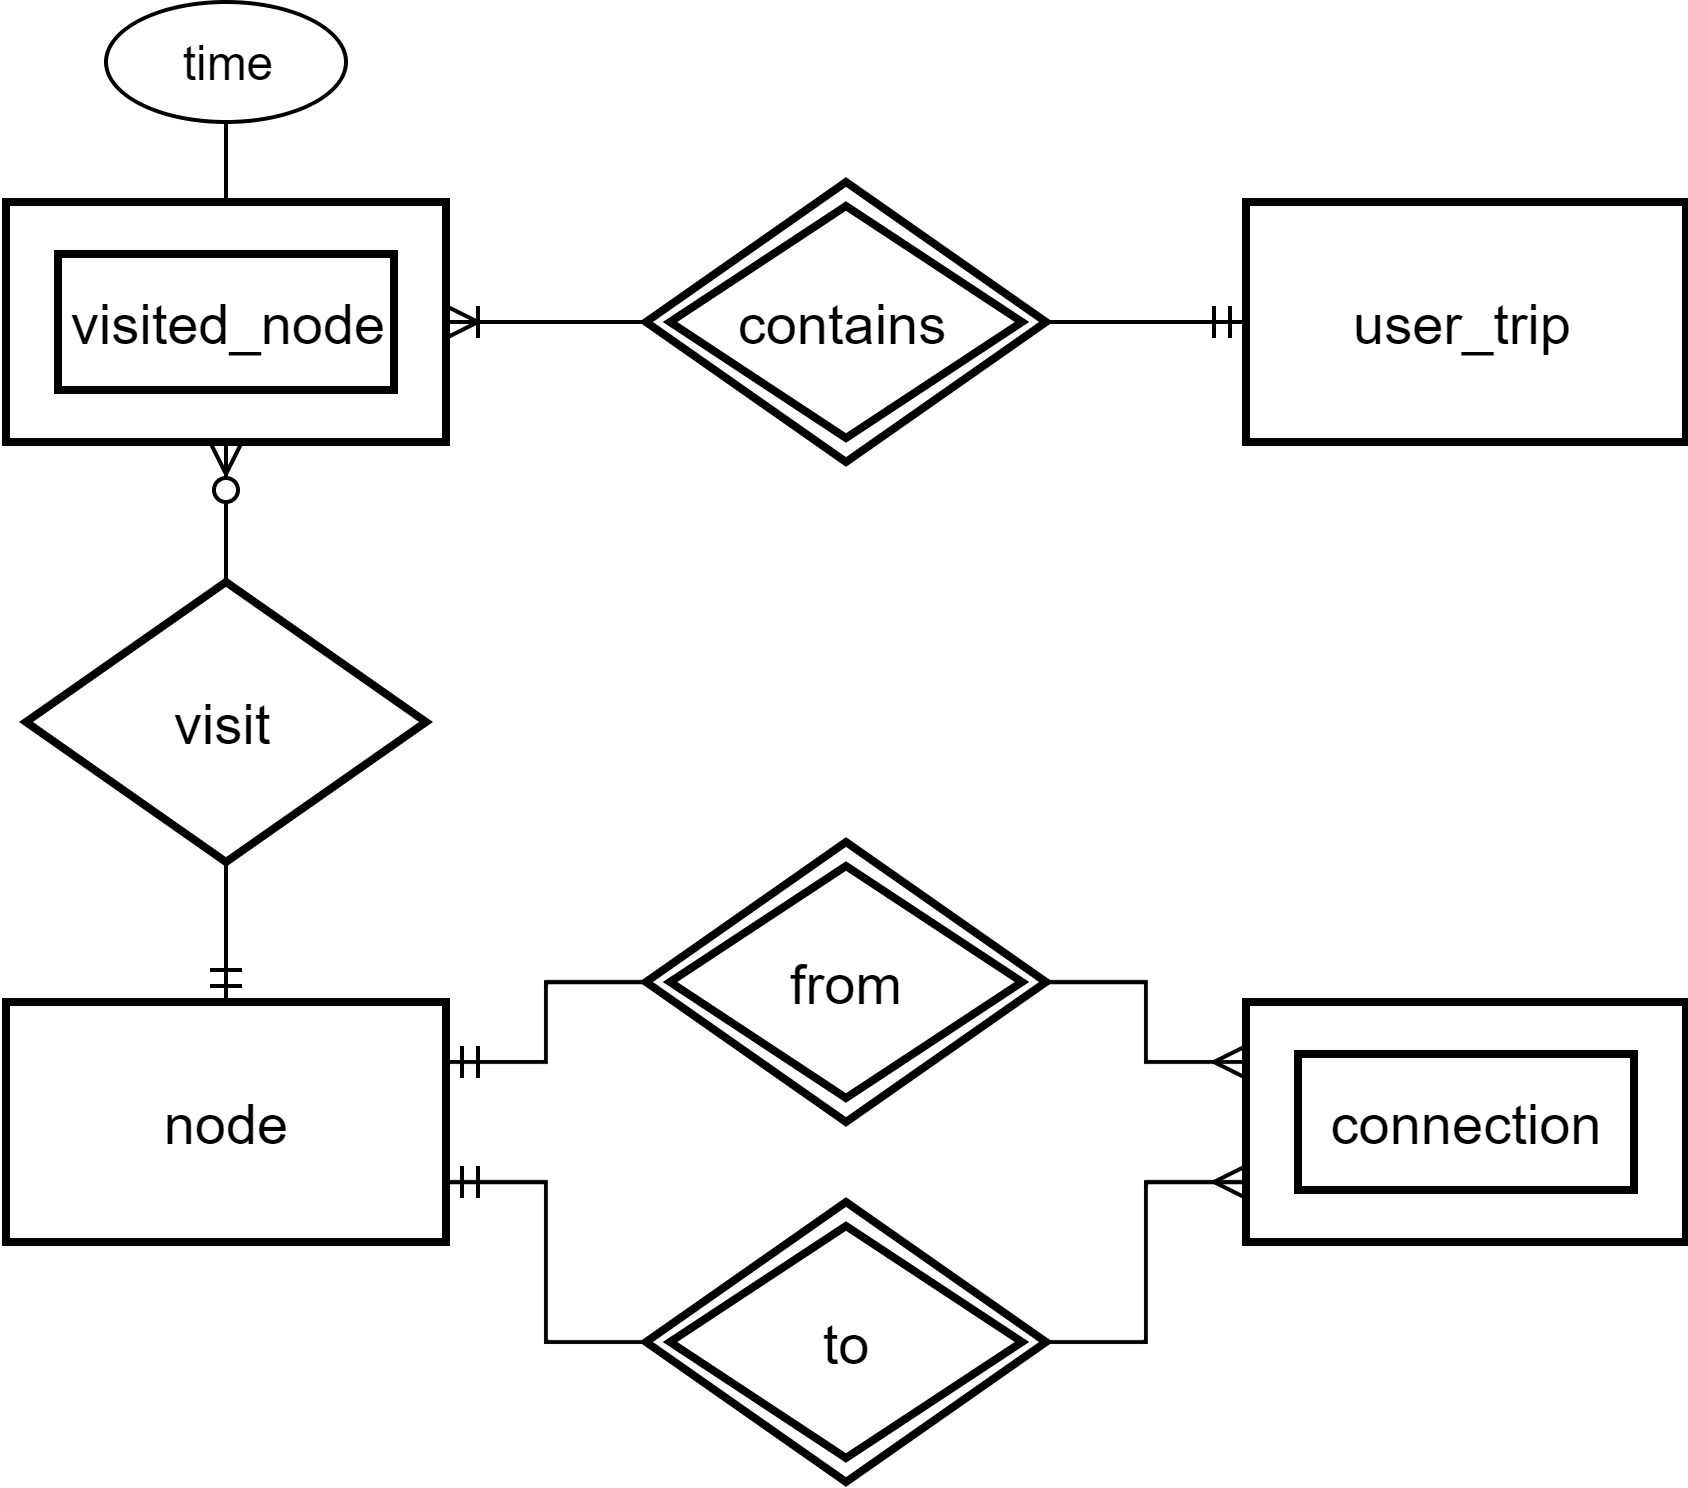
\includegraphics[width=0.6\textwidth]{figures/street_er.png}}
		\end{center}
		\caption{An ER diagram representing the model for user trajectories for \acrshort{ctr}.}
		\label{fig:street_er}
	\end{figure}
    
    Figure~\ref{fig:street_er} contains the entity-relationship diagram of our network model, where nodes and connections define a directed graph, over which user trajectories can be conformed by sequentially visiting the nodes. The order in which these nodes are visited is implicitly defined by the time, meaning that it is necessary to somehow represent that time for the visited nodes of each trajectory.
    %It is easy to see how this model could introduce redundancy in the public transportation context, where several passengers may be sharing the same bus at the same time.
	
	To make the
	use of \gls{csa} possible, we define a trip or trajectory of a moving object
	over a network as the temporally-ordered sequence of the nodes the trajectory
	traverses. An integer $s_i \in S$ is assigned to each node such that a trajectory is a sequence (string) of consecutively nodes visited by a single user. Note that this representation avoids the cost of storing coordinates to represent the location users pass through during a trajectory. It is just enough to identify the stops or nodes and when necessary to map these nodes to geographic locations. Moreover, when the underlying network is formed by street segments, we do not specify at which part of the segment did the trajectory start or finished: we consider such level of detail irrelevant for traffic analysis, as it can be effectively made on a street-segment level.
	
	We then build a \gls{csa}, over the concatenation of
	these strings (trajectories), with some adaptations for this
	specific application. In addition, we discretize the time in periods of fixed
	duration (i.e. timeline split into 5-minute intervals) and each time
	segment is identified by an integer $t_i \in I$. In this way, it is possible
	to store the times when trajectories reach each node by associating the
	corresponding $t_i$ with each node in each trajectory. The sequence of
	times for all the nodes within a trajectory is self-indexed with a \gls{wt}
	to efficiently answer temporal and spatio-temporal queries.

	Among other types of queries, in this work we focus on the following counting queries, which to the best of our knowledge have not been  addressed by previous proposals. In general terms, we define two general queries, number-of-trips queries and top-k queries, upon which we apply spatial, temporal, or spatio-temporal constraint when useful.

	\begin{itemize}
		\item[(a)] {\em Number-of-trips queries.} This is a general type of queries that counts the number of distinct trajectories. When applying spatial, temporal, or spatio-temporal constraints, it can specialized in the following queries:
		
		\begin{enumerate}
			\item Pure spatial queries:
			\begin{itemize}
				\item[-] {\em Number of trips starting at node $X$ (\startX).}
				\item[-] {\em Number of trips ending at node $X$ (\endX).} 
				\item[-] {\em Number of trips starting at $X$ and ending at $Y$ (\XtoY).}
				\item[-] {\em Number of trips using or passing through node $X$. Can also be seen as the average load of the node $X$. (\loadX)}
			\end{itemize}
			
			\item Spatio-temporal queries:
			\begin{itemize}
				\item[-] {\em Number of trips starting at node $X$ during time interval $[t_1..t_2]$ (\startX$_T$).}
				\item[-] {\em Number of trips ending at node $X$ during the time interval $[t_1..t_2]$ (\endX$_T$). }
				\item[-] {\em Number of trips starting at $X$ and ending at $Y$ occurring during  time interval $[t_1..t_2]$ (\XtoY$_T$).} This type of queries is further classified into: 
				\begin{itemize}
				    \item[(i)] \XtoY$_T$ with strong semantics (\XtoY$_{Ts}$), which considers trajectories that completely occur within interval $[t_1..t_2]$.
				    \item[(ii)] \XtoY$_T$ with weak semantics (\XtoY$_{Tw}$), which considers trajectories whose life time overlap $[t_1..t_2]$.
				\end{itemize}
				\item[-] {\em Number of trips using node $X$ during the time interval $[t_1..t_2]$. Can also be seen as the average load of the node $X$ within a given time interval. (\loadX$_T$).}
			\end{itemize}
			
			\item Pure temporal queries:
			\begin{itemize}
				\item[-] {\em Number of trips starting during the time interval $[t_1..t_2]$ (\startT). } 
				\item[-] {\em Total usage (load) of network nodes during the time interval $[t_1..t_2]$ (\loadT).}
				\item[-] {\em Number of trips performed within the time interval $[t_1..t_2]$ (\tripT).} 
			\end{itemize}
		\end{enumerate}
		
		\item[(b)] {\em Top-k queries.} In this type of queries we want to retrieve the $k$ nodes with the highest number of trips. In this case, depending on having a temporal constraint or not we include the following queries:
		\begin{enumerate}
			\item Pure spatial {\em Top-k} queries:
			\begin{itemize}
				\item[-] {\em Top-k most used nodes (\topK)}, that returns the nodes with the largest number of trips passing through.
				\item[-] {\em Top-k most used nodes to start a trip (\topK$_s$)}, that returns the nodes with the largest number of trips that start at that node.
			\end{itemize}
			
			\item Spatio-temporal {\em Top-k}  queries:
			\begin{itemize}
				\item[-] {\em Top-k most used nodes during time interval $[t_1..t_2]$(\topK$_T$)}, that returns the nodes with the largest number of trips passing through within time interval $[t_1..t_2]$. 
				\item[-] {\em Top-k most used nodes to start a trip during time interval $[t_1..t_2]$(\topK$_{Ts}$)}, that returns the nodes with the largest number of trips starting there within time interval $[t_1..t_2]$ at that node.
			\end{itemize}
		\end{enumerate}
	\end{itemize}

\section{Structures}
\label{sec:ctr:str}
	To support the queries seen in Section~\ref{sec:ctr:desc}, we need to represent the spatial and temporal components of our collection of user trips that is coherent with the network model described. Therefore, we will proceed to detail how each trip is described, before we show how that description is implemented in our compact data structures.

	If we consider a network $\mathcal{N}$ with a set of nodes $S$, 
	we can see a dataset of trips $\mathcal{T}$ over $\mathcal{N}$ as 
	a set of trips, where for each trip $\mathcal{T}_i \in \mathcal{T}$, we represent a list with the 
	$n_i$
	temporary-ordered nodes it traverses and the corresponding timestamps: 
	$\mathcal{T}= \{ \langle (s^i_1, s^i_2, \dots,  s^i_{n_i}),(t^i_1, t^i_2, \dots,  t^i_{n_i}) \rangle\}$, $i\in[1..|\mathcal{T}|]$, 
	$s^i_j \in S$, and $t^i_{x} \leq t^i_y, \forall x < y$. 
	Note that every node in the network can be identified with an integer ID $s^i_j \in S$ and that, if we are interested in
	analyzing the usage patterns of the network, we will also be interested in discretizing time into 
	time intervals (i.e. 5-min, 30-min intervals). Therefore,
	we will have $|I|$ different time intervals that can also be identified with an
	integer ID ($t^i_j \in I$).

	The size of the time interval is a parameter for the time-discretizing process
	that can be adjusted to fit the required precision in each domain.
	For example, in a public
	transportation network where we could have data including five years of trips, one
	possibility would be to divide that five-years period into
	10-minute intervals hence obtaining a
	vocabulary of $|I|=5\times 365 \times 24 \times 60/10 = 262,800$ different intervals. 
	Other possibility would
	be to use cyclically annual 10-minute periods resulting in $|I|=262,800 / 5 = 52,560$. 
	However,  in public transportation networks, queries such
	as \textit{``Number of trips using the stop X on May 10 between 9:15 and 10:00''} may be not 
	as useful as queries such as \textit{``Number of trips using stop X on Sundays between 9:15 and
		10:00''}.
	% Therefore, it is more useful
	%to encode with the same codes the hours in working days on one hand and
	%hours in weekend in the other.
	For this reason, \gls{ctr} can adapt how the
	time component is encoded depending on the queries that the system must answer.

	\begin{figure}[ht]
		\begin{center}
			{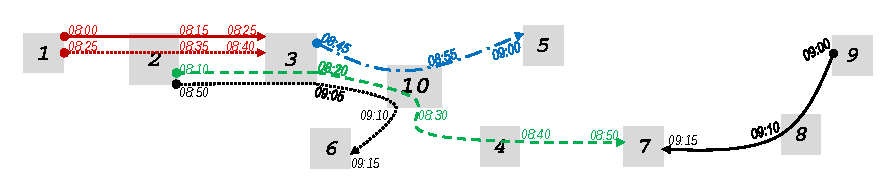
\includegraphics[width=1\textwidth]{figures/network_ctr.eps}}
		\end{center}
		\caption{A set of trips over a network with 10 nodes.}
		\label{fig:network}
	\end{figure}

	\begin{example} \label{exp:ctr}
	Figure~\ref{fig:network} shows a network that contains $|S|=10$ nodes 
	numbered from $1$ to $10$. Over that network we have six trips ($|\mathcal{T}|=6$),
	and, for each of them, we indicate the sequence of nodes it traverses
	and the time when the trip goes through those nodes. If we discretize time into
	5-minute intervals, starting at 08:00h, and ending at 9:20h, we will have
	have $|I|=16$ different time intervals. Any timestamp within
	interval $\mathit{[08\!:\!00,08\!:\!05)}$ will
	be assigned time-code $0$, those within $\mathit{[08\!:\!05,08\!:\!10)}$ code $1$, and so on until
	times within $\mathit{[09\!:\!15,09\!:\!20)}$ that are given time-code $15$.  
	Therefore, our dataset of trips will be: 
	$\mathcal{T}$: $\{$%
	$\langle (\mathbf{1,2,3     })$, $(\mathit{5,7,8})                     \rangle$, 
	$\langle (\mathbf{2,3,10,6  })$, $(\mathit{10,13,14,15})           \rangle$, 
	$\langle (\mathbf{1,2,3     })$, $(\mathit{0,3,5})                     \rangle$, 
	$\langle (\mathbf{2,3,10,4,7})$, $(\mathit{2,4,6,8,10}) \rangle$, 
	$\langle (\mathbf{3,10,5    })$, $(\mathit{9,11,12})                     \rangle$, 
	$\langle (\mathbf{9,8,7     })$, $(\mathit{12,14,15})                    \rangle$$\}$, 
	where bold numbers indicate node IDs and slanted ones indicate times. \qed
	\end{example}

    \medskip
	In \gls{ctr} we represent both the spatial and the temporal component of the trips using well-known
	self-indexing structures in order to provide both a compact representation and the ability to 
	perform fast indexed searches at query time. In Section~\ref{sec:ctr:str:spat} we focus on the
	spatial component and discuss how we adapted  \gls{csa} to deal with trips. We also
	show how we support spatial queries. Then, in Section~\ref{sec:ctr:str:temp} we show that the times,
	which are kept aligned with the spatial component of the trips, can be handled with   
	a \gls{wt}-based representation. Actually we study two alternatives (a \gls{htwt} and a \gls{wm}) 
	and show how temporal and spatio-temporal (Section~\ref{sec:ctr:alg:stq}) queries are supported by \gls{ctr}.

	\subsection{Spatial component using a CSA}
	\label{sec:ctr:str:spat}
	We use a slightly adapted \gls{csa} to represent the spatial component of our dataset of trips within \gls{ctr}. 
	However, we must perform some preprocessing on each trip  $\mathcal{T}_i \in \mathcal{T}$ before building a \gls{csa} on it. Initially, we sort the trips by their first node ($s^i_1$), then by the last node ($s^i_n$), then by the starting time ($t^i_1$), and finally, by its second node ($s^i_2$), third node ($s^i_3$), and successive nodes (i.e. the trips are sorted by the key $s_1,s_n,t_1,s_{2..n-1}$.  Note that the start time ($t^i_1$) of the trip does not belong to the spatial component, but it is nevertheless used for the sorting.\footnote{This initial sorting of the trips will allow us to answer some useful queries very efficiently  (i.e., count trips starting at node $X$ and ending at node $Y$).}

	Following with Example~\ref{exp:ctr}, after sorting the trips in $\mathcal{T}$ with the criteria above, 
	our sorted dataset $\mathcal{T}^s$ would look like: 
	$\mathcal{T}^s$: $\{$%
	$\langle (\mathbf{1,2,3     })$, $(\mathit{0,3,5})                     \rangle$, 
	$\langle (\mathbf{1,2,3     })$, $(\mathit{5,7,8})                     \rangle$, 
	$\langle (\mathbf{2,3,10,6  })$, $(\mathit{10,13,14,15})           \rangle$, 
	$\langle (\mathbf{2,3,10,4,7})$, $(\mathit{2,4,6,8,10}) \rangle$, 
	$\langle (\mathbf{3,10,5    })$, $(\mathit{9,11,12})                     \rangle$, 
	$\langle (\mathbf{9,8,7     })$, $(\mathit{12,14,15})                    \rangle$$\}$. 
	Note that  $ (\mathbf{2,3,10,6  })$ appears before $(\mathbf{2,3,10,4,7})$ because
	during the sorting process we compare $ (\mathbf{2,6,\mathit{2},3, 10,6  })$ with $ (\mathbf{2,7,\mathit{10},3, 10,4,7})$;
	that is, we compare the starting nodes ($\mathbf{2}$ and $\mathbf{2}$) and then the ending nodes ($\mathbf{6}$ and $\mathbf{7}$).
	If needed  (not in this example) we would have also compared the slanted values ($\mathit{2}$ and $\mathit{10}$) 
	that are the starting times of the trips, and finally the rest of nodes  ($ \mathbf{3, 10,6  }$ and $ \mathbf{3, 10,4,7}$).
	Similarly, the two trips containing nodes $ (\mathbf{1,2,3})$ are sorted by the starting times ($\mathit{0}$ and $\mathit{5}$).


	In a second step, we enlarge all the trips $\mathcal{T}^s_i \in \mathcal{T}^s$ with a fictitious terminator-node $\$_i$ whose
	timestamp is set to that of the initial node of the trip. We choose terminators such that $\$_i \prec \$_j, \forall i<j$; 
	that is, the lexicographic value of $\$_i$ is smaller for smaller $i$ values. In addition, the lexicographic value
	of any terminator must be lower than the ID of any node in a trip. Therefore, an enlarged trip $\mathcal{T}^s_i$
	would become $\mathcal{T}'_i =  \langle (s^i_1, s^i_2, \dots,  s^i_{n_i}, 
	\mathbf{\$_i}),(t^i_1, t^i_2, \dots,  t^i_{n_i}, \mathbf{t^i_1}) \rangle$. 

	The next step involves concatenating the codes $s^i_j$ and $\$_i$ of the spatial components of our trips and to add an 
	extra trailing terminator $\$_0$ to create a sequence $Text[1..n]$.\footnote{By definition, it must hold that $n = |\mathcal{T}| + 1 + \displaystyle\sum^{|\mathcal{T}|}_{i=1} n_i$.} $\$_0$ must be  lexicographically 
	smaller than any other entry (then it also holds $\$_0 \prec \$_i$, $\forall i \in [1..|\mathcal{T}|]$). In the top part of
	Figure~\ref{fig:tcsa}, we can see array $Text$ for the running example, as well as the corresponding time-IDs that
	are regarded in sequence $Icode$  ($Time$ shows the original times).
	
	\begin{figure}[ht]
	  \begin{center}
	  {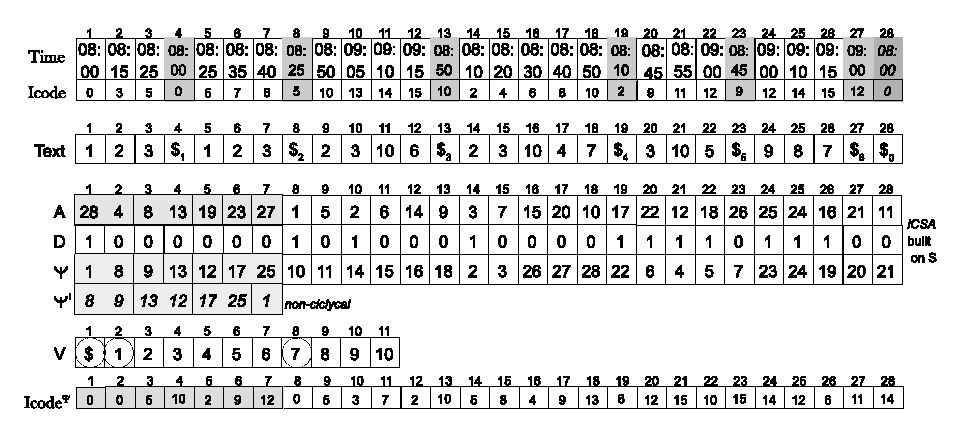
\includegraphics[width=1.00\textwidth]{figures/csttr.eps}}
	  \end{center}
	  \caption{Structures involved in the creation of a \acrshort{ctr}.}
	  \label{fig:tcsa}
	\end{figure}

	Finally, we build a \gls{csa} on top of $Text$ to obtain a self-indexed representation of the spatial component in \gls{ctr}.
	Figure~\ref{fig:tcsa} depicts the structures $\Psi$ and $D$ used by the \gls{csa} built over $Text$. There is also a vocabulary
	$V$ containing a $\$$ symbol and the different node IDs in lexicographic order.

	Note that the use of different values $\$_i$ as terminators ensures that our sorting criteria are kept even if we follow the
	standard suffix-sort procedure\footnote{The suffix $Text[i..n]$ is compared with the suffix $Text[j..n]$.} 
	required to build suffix array $A$ during the creation of \gls{csa}. Yet, when we finish that
	process, we can replace all these $1+|\mathcal{T}|$ terminators $\$_i$ by a unique $\$$. This is the reason why there is only one $\$$ symbol in $V$. 
	 
	%while in $V$ there is only one single entry for all the $\$$. 
	%The use of different values for $\$_i$ during the sorting explains why $A[22] = 18$ is placed before $A[23]= 26$. Note that
	%the suffix starting at $S[18]$ is ``$7 \cdot \$_4 \cdot 2 \cdot 3 \dots$'' and that suffix at
	%$S[26]$ is ``$7 \cdot \$_6 \cdot 9 \cdot \dots$''. Therefore, it holds that $A[22] \prec A[23]$. However, considering
	%the traditional definition of a {\em suffix}, these suffixes would be ``$7 \cdot \$_4 \cdot 3 \cdots $''
	%and ``$7 \cdot \$_6 \cdot \$_0 \cdots $'' respectively,  and  $A[22] \prec A[23]$ would not hold.

	Although they are not needed in \gls{ctr}, we show also suffix array $A$ and $\Psi$' for clarity reasons in Figure~\ref{fig:tcsa}. 
	$\Psi'$  contains the first entries of $\Psi$ from a regular \gls{csa}, whereas we introduced a small variation
	in \gls{ctr} for entries $\Psi[1..(|\mathcal{T}|+1)]$. Displaying both $\Psi$ and $\Psi'$ helps us to better illustrate our process to build $\Psi$. 
	For example, $A[8]=1$ points to the first node of the first trip $S[1]$.
	$\Psi[8]=10$ and $A[10]=2$ point to the second node.  $\Psi[10]=14$ and $A[14]=3$ point to the third node.
	$\Psi[14]=2$ and $A[2]=4$ point to the ending $\$_1$ of the first trip. Therefore, in the standard 
	\gls{csa}, $\Psi'[2]=9$ and $A[9]=5$  point to the first node of the second trip. 
	However, in  \gls{ctr}, $\Psi[2]=8$ and $A[8]=1$ point
	to the first node of the first trip. With this small change, subsequent applications of $\Psi$ will allow 
	us to cyclically traverse the nodes of the trip instead of accessing the following entries of $Text$.

	Another interesting property arises from the use of a cyclical $\Psi$ on trips, and from using trip terminators.
	Since the first entries in $\Psi[2..|\mathcal{T}|+1]$ correspond the $\$$ symbols that 
	mark the end of each trip in $Text$ (remember that $\Psi[1]$ corresponds the $\$_0$), we can see that the $j$-th node of the $i$-th trip can
	be obtained as $V[\rank_1(D, \Psi^j[i+1])]$, (where $\Psi^3[x]= \Psi[\Psi[\Psi[x]]]$). This property
	makes it very simple to find starting nodes for any trip.
	For example, if we focus on the shaded area $\Psi[2..7]$, we can find the ending terminator $\$_4$ of the
	fourth trip at the $5$-th position (because the first $\$_0$
	corresponds to the final $\$$ at $S[28]$). Therefore, its starting node can be found 
	as $V[\rank_1(D, \Psi[4+1])]$. Since $\Psi[5] = 12$ and $\rank_1(D,12)= 3$, 
	the starting node is $V[3]=\mathbf{2}$. For illustration purposes note that it would correspond to $Text[A[12]]$.
	By applying $\Psi$ again, the next node of that trip would be obtained by computing $\Psi[12] = 16$, 
	$\rank_1(D,16)=4$, and accessing $V[4]=\mathbf{3}$  (that is, we have obtained 
	 $V[\rank_1(D, \Psi[\Psi[4+1]])]=\mathbf{3}$, and so on. 

	Regarding the space requirements of the \gls{csa} in \gls{ctr}, we can expect to obtain a good compressibility
	due to the structure of the network, and the fact that trips that start in a given node or simply
	those going through that node will probably share the same sequence of ``next'' nodes. This will
	lead us to obtaining many {\em runs} in $\Psi$~(\cite{NM07}), and consequently good compression could be expected.

	\subsubsection{Implementation details} In our implementation of \gls{csa}, we used the
	$iCSA$\footnote{\url{http://vios.dc.fi.udc.es/indexing}} from \cite{FBNCPR12} briefly discussed 
	in Section~\ref{sec:csa}. Yet, we introduced some small modifications:

	\begin{itemize}
		\item The construction of the Suffix Array $A$ is done with 
		{\em SA-IS} algorithm~\cite{nong2011two}.\footnote{We have used the improved implementation by Yuta Mori, available at \url{https://sites.google.com/site/yuta256/sais}} 
		In comparison with the  {\em qsufsort} algorithm\footnote{
			\url{http://www.larsson.dogma.net/research.html}}
		%\footnote{https://github.com/y-256/libdivsufsort/}
		\cite{Larsson:2007:FSS:1314704.1314853} used in the original $iCSA$, it achieves a linear time construction 
		and a lower extra working space. Refer to \cite{magiera2019sacabench} for an up to date comparison among the modern Suffix Array construction methods.
		
		\item In  $iCSA$, a plain representation for bitvector $D$ was used, with additional structures to support
		$\rank_1$ in constant time using ($0.375\times n$ bits). With that structure, they could solve $\select$ in $O(\log n)$ time (yet 
		they did not actually needed solving $\select$ in $iCSA$).
		In our \gls{csa}, we have used the {\em SDArray} from \cite{okanohara2007practical} to represent $D$. It provides a very 
		good compression for sparse bitvectors, as well as constant-time $\select_1$ operation.
		
		\item In \cite{FBNCPR12}, $\bsearch(\Psi,P)$ operation was implemented with a simple binary search over $\Psi$ rather than
		using the backward-search optimization proposed in the original \gls{csa} \cite{Sad03}. In our proposals, we used
		backward search since it led to a much lower performance degradation at query time when a sparse sampling of $\Psi$ 
		was used.
		
		%We implemented a backward search for the $\bsearch$ operation in the \gls{csa}. When the pattern $P[1..p]$ is searched, 
		%we start by locating the ranges for $P[p]$ and $P[p-1]$ in $D$. After that, we binary search over $\Psi$ for the symbols
		%in $P[p-1]$ that point to $P[p]$, getting a narrower range. We repeat it recursively until reaching $P[1]$. The main
		%advantage of the backward search in this situation is that we have more control on the accesses on the compressed 
		%$\Psi$, making it possible to search over the samples first, and narrowing that search down to a single compressed 
		%block in each cell, instead of having to rely on random access for long patterns.
	\end{itemize}

	\subsection{Time intervals representations}
	\label{sec:ctr:str:temp}

	In this section, we focus on the temporal component associated with each node of the enlarged trips $\mathcal{T}'_i$ 
	in our dataset, previously described in Section~\ref{sec:ctr:str:spat}. Recall that in Figure~\ref{fig:tcsa}, sequence $Time$ contains the discretized time intervals
	associated with each visited node in a trip, and $Icode$ a possible encoding of times.
	In \gls{ctr} we focus on the values in $Icode$, yet, since $Text$ is not kept anymore in \gls{ctr}, we 
	reorganize the values in $Icode$ to keep them aligned with $\Psi$ rather than with $Text$. Those
	values are represented within array $Icode^{\Psi}$ in Figure~\ref{fig:tcsa}. 
	For example, we can see that $Icode^{\Psi}[4]$ corresponds with $Icode[A[4]]=10$, 
	$Icode^{\Psi}[15]$ corresponds with $Icode[A[15]]=8$, and so on. Conveniently, the first $|\mathcal{T}| + 1$ entries of $Icode^{\Psi}$ will contain the time interval codes for the start of each trip, as each $\$_i$ was originally aligned with a copy of the first time interval $t^i_1$ of each trip.

	Aiming at having a compact representation of $Icode^{\Psi}$ while permitting fast 
	access and resolution of range-based queries (that we could use to search for trips within 
	a given time interval), we have considered two \gls{wt}-based alternatives from the ones presented in Section~\ref{sec:wt}:

	\begin{itemize}
	  \item A Wavelet Tree using variable-length Hu-Tucker codes (\gls{htwt}).
	  Recall this is the \gls{wt} variant that permits to compress the original symbols with \mbox{variable-length} codes and 
	  still supports $\cnt_{a,b}(S,i,j)$ operation in $O(log~\sigma)$ time. Since Hu-Tucker coding assigns shorter codes
	  to the most frequent symbols, the compression of our \gls{htwt} is highly dependent of the distribution
	  of frequencies for the $Icode^{\Psi}$. Yet, if our 
	  trips represent movements of single users in a transportation network, we could expect to observe two or more periods 
	  corresponding to rush hours within a single day (see Section~\ref{sec:ctr:exp:data}). This would lead to obtaining a skewed distribution of the frequencies 
	  for the symbols in $Icode^{\Psi}$, and consequently, we could expect to have better compression than if we used a 
	  balanced \gls{wt}. The expected number of bits of our \gls{htwt} is $nH_0(Icode^{\Psi})$.

	  \item A balanced Wavelet Matrix (\gls{wm}). As we have shown in Section~\ref{sec:wt}, the \gls{wm} is typically the most
	  compact uncompressed variant of \gls{wt} and it is faster than a pointerless \gls{wt}. This is the reason why we chose
	  a balanced \gls{wm} instead of a balanced \gls{wt} as this second alternative. Recall that, $Icode^{\Psi}$ contains $n$ symbols, 
	  and each symbol can be encoded with $\log  |I|$ bits, hence the 
	  balanced \gls{wm} can be seen as a matrix of $n  \log|I|$ bits.
	\end{itemize}
	
	\begin{figure}[ht]
		\begin{center}
			{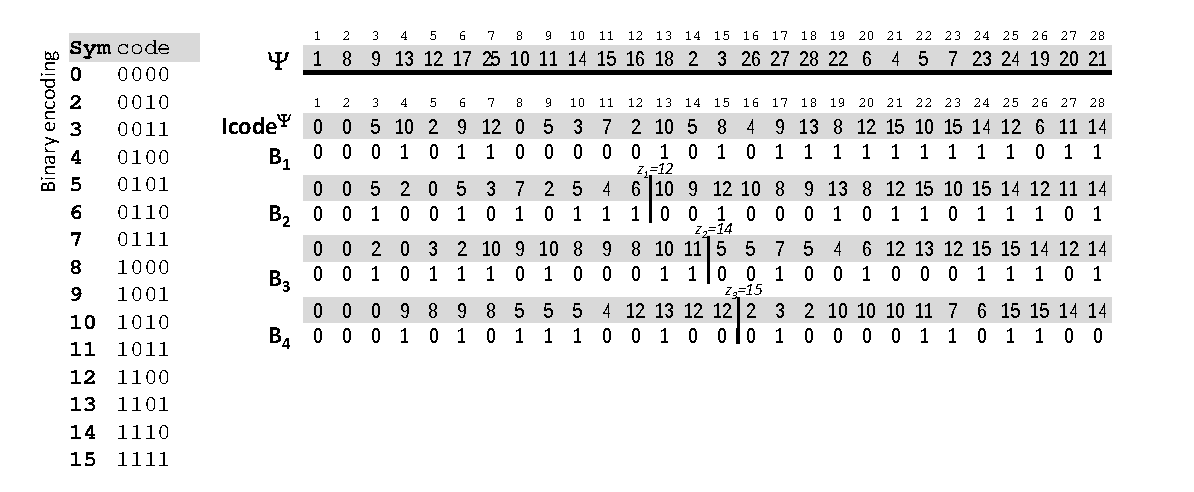
\includegraphics[width=1.0\textwidth]{figures/wma.eps}}
			{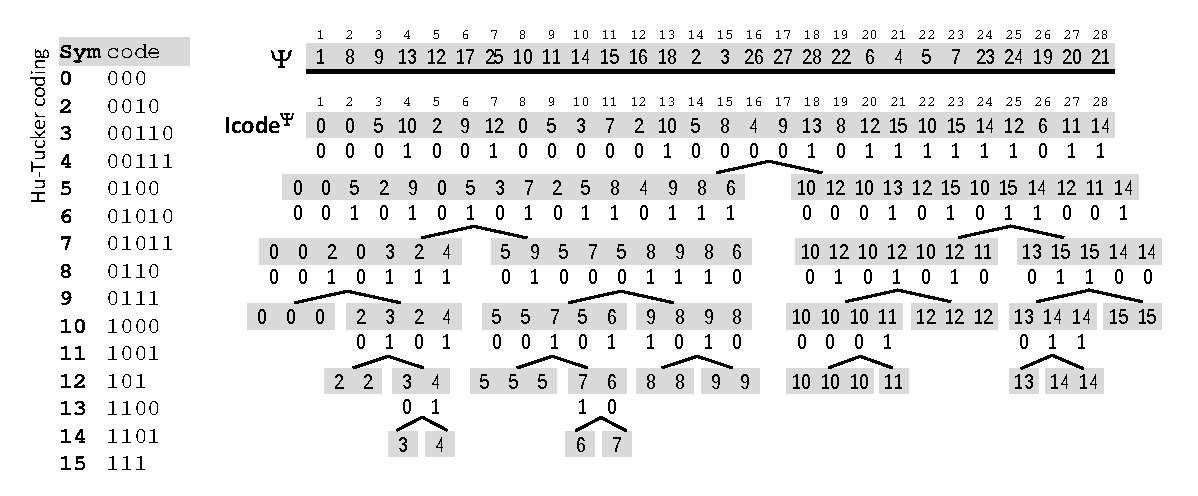
\includegraphics[width=1.0\textwidth]{figures/wta.eps}}
		\end{center}
		\caption{Balanced \acrshort{wm} (top) and \acrshort{htwt} (bottom).}
		\label{fig:wtwm}
	\end{figure}


	In Figure~\ref{fig:wtwm}, we show both the \gls{wm} and the \gls{htwt} built on top of $Icode^{\Psi}$ from Figure~\ref{fig:tcsa}.
	The binary code-assignment to the source symbols $t_i \in I$ and that obtained after applying Hu-Tucker encoding
	algorithm~\cite{hu1971optimal} are also included in the figure.
	
	Since the most useful operation of these two structures for our application is, by far, $\cnt_{a,b}(Icode^{\Psi},i,j)$, we will proceed to explain in detail how the efficiency of that operation has influenced our choice of structures. Just as proven in Section~\ref{sec:wt} with \gls{wt}, both \gls{htwt} and \gls{wm} implement the $\cnt_{a,b}(Icode^{\Psi},i,j)$ operation in $O(\log~\sigma)$ time on average. This is easy to prove for \gls{htwt} as each node will contain entries from a lexicographically contiguous subrange from the alphabet $\Sigma$, making the same properties seen for \gls{wt} hold. The main difference is that Hu-Tucker codes will reshape the tree, making the leaves containing the least frequent symbols deeper than the leaves with the more frequent symbols, which may theoretically produce a tree of height $\sigma-1$,\footnote{Assume a vocabulary $\Sigma=\{s_1,...,s_\sigma\}$, where the probability of appearance of the symbol $s_i$ in the text $S$ turned out to be $2^{-i}$.} which will obviously affect the worst-case performance, in exchange of an improved compression ratio.

	The complexity may seem initially harder to analyze for \gls{wm}, as its ``nodes'' are delimited implicitly: the symbols with a code starting with a 0 will find their second bit in an implicit node delimited by the subrange $B_2[1..z]$ (for some $1 \leq z < n$), while the symbols with a code starting with a 1 will correspond to $B_2[z+1..n]$. Generalizing this idea, we can assert that symbols with the same \textit{context} of $\alpha$ starting bits in their codes will find their next $\alpha+1$ bit in some subrange $B_{\alpha+1}[i..j]$ with $1 \leq i \leq j \leq n$. Therefore, the same properties from \gls{wt} can be exploited for a $\cnt_{a,b}(Icode^{\Psi},i,j)$ operation in \gls{wm} as well, allowing us to solve it in $O(\log\sigma)$ worst-case time.

	While it would also be possible to build \gls{wm} using canonical Huffman codes, it is unfortunately impossible to guarantee the $O(\log\sigma)$ bound on $\cnt_{a,b}(Icode^{\Psi},i,j)$ on such \gls{wm}, as the symbols lose their original lexicographic proximity, meaning that symbols which would appear on the same node of \gls{wt} due to the common most significant bits in their original codes, would get different Huffman codes based on their frequency of appearance in the text, ending up in separate nodes. On the other hand, to the best of our knowledge, there is no practical way of building \gls{wm} with Hu-Tucker codes.

	\subsubsection{Implementation details} 
	\label{sec:ctr:str:time:imp}
	%We include here details regarding how we tune our \gls{htwt} and \gls{wm}.
	As we discussed in Section~\ref{sec:wt}, both \gls{htwt} and \gls{wm} are built over bitvectors that require support for $\rank$ and $\select$ operations. In our implementations we included two alternative bitvector representations avaliable
	at {\em libcds} library:{\footnote{\url{https://github.com/fclaude/libcds}}}
	
	\begin{itemize}
		\item A plain bitvector based on \cite{Mun96} named {\em RG} with 
		additional structures to support $\rank$ in constant time ($\select$ in logaritmic time).
		{\em RG} includes a sampling parameter ($factor$) that we set to value $32$. In this case,
		our  bitvector {\em RG} uses $n (1+1/32)$ bits. That is, we tune {\em RG} to use a sparse sampling. 
			
		\item A compressed RRR bitvector~\cite{Raman:2002:SID:545381.545411}. The {\em RRR} implementation includes
		a sampling parameter that we tune to values $32$, $64$, and $128$. Higher sampling values typically achieve better compression.
	\end{itemize}


	In advance, when presenting results for \gls{htwt} and \gls{wm} we will consider the four bitvector configurations
	above. Regarding our implementations of \gls{wm} and \gls{htwt}, note that we reused the same implementation of \gls{wm} from \cite{CNO15}, 
	and we created our custom \gls{htwt} implementation, paying special focus at solving $\cnt_{a,b}(Icode^{\Psi},i,j)$ efficiently.

\section{Algorithms} \label{sec:ctr:alg}
	In this section, we discuss how our previously described structures can solve the queries proposed in Section~\ref{sec:ctr:desc}. We also include a brief complexity analysis for some of the cases.

	\subsection{Spatial queries}
	\label{sec:ctr:alg:sq}

	With the \gls{csa} structure described for representing the spatial component of the trips,
	the following queries can be solved.

	\begin{itemize}
	\item {\em Number of trips starting at node $X$ (\startX).}
	Because $\Psi$ was cyclically built in such a way that every $\$$ symbol is followed by the first node 
	of its trip, this query is solved by $[l..r]\leftarrow\bsearch(\Psi,\$X)$ over the \gls{csa}, 
	which results on a binary search for the pattern $\$X$ over the section $\Psi[2..|\mathcal{T}|]$ corresponding to $\$$ symbols. 
	Then $r-l+1$ gives the number of trips starting at $X$.
	Applying the backward search algorithm for \gls{csa}, this query involves two $\select_1$ operations over $D$ in order to delimit the region $\Psi[l_x..r_x]$ for $X$\footnote{Assuming that $X$ is at position $p$ in the vocabulary $V$ of \gls{ctr} ($V[p]=X$), its region in $\Psi[l_x..r_x]$ is obtained as $l_x \leftarrow \select_1(D,p)$,  $r_x \leftarrow \select_1(D,p+1)$. If $p$ is the last entry in $V$, we set $r_x \leftarrow n$.} and one binary search in the $\$$ region to find the subrange for $\$X$. Since $\select_1$ on $D$ are $O(1)$, the temporal complexity of this query is $O(\log|\mathcal{T}|)$, omitting a constant factor due to the compression of $\Psi$.

	\item {\em Number of trips ending at node $X$ (\endX).} In a similar way to the previous query, this one can be answered with $\bsearch(\Psi,X\$)$. It will require four $\select_1$ operations (still $O(1)$) and a binary search over the $X$ region, giving a total worst-case complexity of $O(\log (n - |\mathcal{T}|)) \subset O(\log n)$.

	\item {\em Number of trips starting at $X$ and ending at $Y$ (\XtoY).}
	Combining both ideas from above, and thanks to the cyclical construction of $\Psi$, this query is solved using $\bsearch(\Psi,Y\$X)$. As it requires two binary searches, the first one to delimit the $\$X$ region and the second one to find the entries within $Y$ that point to that $\$X$ region, the overall complexity is $O(\log n)$.

	\item {\em Number of trips using node $X$ (\loadX).}
	Even though we could solve this query with $\bsearch(\Psi,X)$, it is more efficient to solve it by directly operating on $D$, by finding the region $\Psi[l..r]$ for $X$ and calculating $r-l+1$. All the operations involved are $O(1)$.
	 %Assuming that $X$ is at position $p$ in the vocabulary $V$ of  \gls{ctr} ($V[p]=X$), its total frequency is obtained by $occs_X \leftarrow select_1(D,p+1) - select_1(D,p)$. %That is, we find the range in $D$ corresponding to the node $X$.
	%If $p$ is the last entry in $V$, we set $occs_X \leftarrow n+1-select_1(D,p)$.

	\item {\em Top-k most used nodes (\topK).}
	We provide two possible solutions for this query named: a sequential and a binary-partition approach:

	\begin{itemize}
	\item The {\em sequential} (\topK$_{seq}$) approach is the simpler alternative to compute the $k$ most used nodes.
	The idea is	to apply  $\select_1(D,i)$ operations sequentially for every $i \in [2..|V|$ to compute the 
	frequency of each node and to return the $k$ nodes with highest frequency.
	We use a min-heap that is initialized with
	the first $k$ nodes, and for every node $s$ from $k+1$ to $|V|$, 
	we compare its frequency with that of the minimum node (the root) from
	the heap. In case the frequency of $s$ is higher, the root of the heap is replaced by $s$ and
	then moved down to comply with the heap ordering. At the end of the process, the heap
	will contain the top-k most used nodes $\langle p_1\:,\:p_2,\:\dots,\:p_k \rangle$, which can be 
	sorted with the heapsort algorithm if needed. 
	%Finally, we return $\langle V[p_1],V[p_2],\dots,V[p_k]\rangle$.
	Note that, since $|S| = |V|-1$, this approach will perform $|S|$ $\select_1$ operations on $D$, as well as up to $|S|$ insertions in the heap of size $k$, thus having an overall complexity of $O(|S|\log k)$.

	\item The {\em binary-partition} (\topK$_{bin}$) approach takes advantage of the skewed 
	frequency distribution for the nodes that trips traverse.  Working over $D$ and $V$, we 
	recursively split $D$  into two segments after each iteration. 
	If possible, we leave the same number of different nodes in each side of the partition. 
	Initially, we start considering the range in $D[l..r] \leftarrow D[\select_1(D,2)..n]=D[|\mathcal{T}|+2..n]$ 
	which corresponds to the nodes that appear in 
	$V$ from positions $i=2$ to $j=|V|$.\footnote{We skip the $\$$ at the first entry of $V$ and its corresponding 
	entries in $D$; that is, $D[1..\select_1(D,2)-1]$.}
	%	$D$ (without its initial range 	%of $|V|$ $\$$ symbols).
	We use a priority queue that is initialized as $Q \leftarrow (\langle i,j\rangle, \langle l,r\rangle)$.
	Then, assuming $m=i + \frac{j-i+1}{2}$ and $q=\select_1(D,m)$, we create two partitions 
	$D[l..q-1]$ and  $D[q..r]$, which correspond respectively to the nodes in $V[i..m-1]$ and $V[m..j]$.
	These  segments created after the partitioning step are
	pushed into  $Q$. %, storing the initial and the final positions of the segment in $D$,
	%and also the initial and final corresponding positions in $V$. 
	The pseudocode can be found in Algorithm~\ref{alg:topk_nieves}.

	The priority of each segment in $Q$ is
	directly the size of its range in $D$ ($r-l+1$). 
	When a segment extracted from $Q$ represents the instance of only one node ($(\langle i,j\rangle, \langle l,r\rangle)$, with $i=j$),
	that node is returned as a result of the top-k algorithm (we return $V[i]$). The algorithm stops when the first $k$ nodes are found.

	For example, when searching for the top-1 most used nodes in the example from Figure~\ref{fig:tcsa}, $Q$ is initialized with
	the segment $[8..28]$, corresponding to nodes from~1~to~10 (positions from~2~to~11 in $V$). Note
	that the entries of $D$ from~1~to~7 and $V[1]$ represent the $\$$ symbol. Since it is not an actual node, it
	 must be skipped. Then $[8..28]$ is split producing the segments $[8..20]$ for nodes 1~to~5 ($V[2..6]$)
	and $[21..28]$ for nodes~6~to~10 ($V[7..11]$). After three more iterations, we extract
	$(\langle 3,3\rangle, \langle 14,18\rangle)$, hence obtaining the segment $[14..18]$ for
	the single node 3 (position $4$ in $V$), concluding that the  {\em Top-1 most used node} is 
	$\mathbf{3}=V[4]$ with a frequency equal to $5=18-14$.
	
	Even though the worst-case complexity of this approach is $O(|S|\log|S|)$, which can be expected when the distribution of nodes is uniform, it can perform considerably better than the sequential approach with a skewed distribution and a small $k$, as will be experimentally proven in Section~\ref{sec:ctr:exp:queries:spat}.

	%\marginpar{\tiny algorithm ten que comezar metendo $<2,|V|>$, non $1,V$}
	%\marginpar{\tiny $q$ debe ser $\select_1(D,m)$, non $\select_1(D,m+1)$}


	%	\begin{figure}[t]
	%	%\vspace{-0.5cm}
	%	\begi%n{center}
	%	\begin{minipage}{0.5\textwidth}
	%	\begin{code}
	%	\textbf{GetTopK} $(k)$: \\
	%	 \> $ Q ~\leftarrow$ \textbf{new PriorityQueue()}; \\
	%	 \> $ Q .$\textbf{push$(<1, |V|>, <$\select$_1(D,2), n-1>)$}; \\
	%	 \> $ current\_k ~\leftarrow 0$; \\%\\
	%	
	%	 \> \textbf{while }$current\_k < k$: \\
	%	 \> \> $ (<i,j>, <l,r>) ~\leftarrow ~Q.$\textbf{pop$()$}; \\%\\
	%	
	%	  \> \> \textbf{if} $i = j$: \\
	%	 \> \> \> $ topK[current\_k] ~\leftarrow i$; \\
	%	 \> \> \> $ current\_k ~\leftarrow current\_k + 1$; \\
	%	 \> \> \textbf{else}: \\
	%	 \> \> \> $ m ~\leftarrow i + \frac{j - i + 1}{2}$; \\
	%	 \> \> \> $ q ~\leftarrow$ \textbf{select$_1(D,m + 1)$}; \\
	%	 \> \> \> $ Q .$\textbf{push$(<i, m-1>, <l, q-1>)$}; \\
	%	 \> \> \> $ Q .$\textbf{push$(<m, j>, <q, r>)$}; \\%\\
	%	 %
	%	 \> \textbf{return} $topK$; \\
	%	\end{code}
	%	\end{minipage}
	%	\end{center}
	%	\vspace{-0.2cm}
	%	\caption{Top K most used nodes implementation using binary partitions}
	%	\label{fig:topk_nieves}
	%	%\vspace{-0.5cm}
	%	\end{figure}

	\end{itemize}


    \begin{algorithm}[ht]
    \SetKwData{k}{k}\SetKwData{topK}{topK}\SetKwData{Q}{Q}\SetKwData{D}{D}\SetKwData{V}{V}\SetKwData{n}{n}\SetKwData{currentK}{current\_k}\SetKwData{k}{k}\SetKwData{i}{i}\SetKwData{j}{j}\SetKwData{l}{l}\SetKwData{r}{r}\SetKwData{middle}{m}\SetKwData{q}{q}
    \SetKwFunction{GetTopK}{GetTopK\_most\_used\_nodes}\SetKwFunction{Push}{Push}\SetKwFunction{Pop}{Pop}
    \SetKwProg{Fn}{Function}{\string:}{}
     
    \Fn{\GetTopK{\k}}{
        \KwData{number \k}
        \KwResult{\topK nodes}
        \BlankLine
        
        \Q $~\leftarrow$ \textbf{new PriorityQueue()}\;
        \Push{\Q,$(\langle2, |\V|\rangle, \langle\select_1(\D,2), \n\rangle)$}\;
        \currentK $~\leftarrow~0$\;
        \BlankLine
        
        \While{\currentK $<$ \k}{
            $(\langle \i,\j\rangle, \langle \l,\r\rangle) ~\leftarrow ~$\Pop{\Q}\;
            \BlankLine
            
            \eIf{\i=\j}{
                $\topK[\currentK]$ $~\leftarrow~\V[\i]$\;
                \currentK $~\leftarrow~\currentK+1$\;
            }{
                \middle $~\leftarrow\i + \frac{\j-\i+1}{2}$\;
                \q $~\leftarrow~ \select_1(\D,\middle+1$)\;
                \Push{\Q,$(\langle \i, \middle-1 \rangle, \langle \l, \q-1 \rangle)$}\;
                \Push{\Q,$(\langle \middle, \j \rangle, \langle \q, \r \rangle)$}\;
            }
        }
        \Return{\topK}\;
     }
     
	\caption{Algorithm {\em Top-k most used nodes} using binary-partition approach.}
	\label{alg:topk_nieves}
	\end{algorithm}

	\item {\em Top-k most used nodes to start a trip (\topK$_s$).}
	Both \topK\ approaches above can be adapted for answering \topK$_s$.
	However, unlike its simpler variant, it requires performing $\bsearch(\Psi,\$X)$ over $\Psi$ (rather than a $\select_1$ on $D$) at
	each iteration, hence increasing the temporal complexity of the operation.

	The implementation of the linear approach is straightforward. The binary-partition approach differs slightly 
	from Algorithm~\ref{alg:topk_nieves}: in \textit{line 3} we have insert $(\langle 2, |V| \rangle, \langle 2,z+1 \rangle)$ into $Q$, and we 
	replace \textit{line 12} with $[x..y]\leftarrow\bsearch(\Psi,\$V[m])$; $q \leftarrow x$. This increases the temporal complexity of \topK$_s$ by a factor of $O(\log n)$ over the complexities discussed for the original \topK\ queries.
	\end{itemize}

	\subsection{Temporal queries}
	\label{sec:ctr:alg:tq}
	With either one of the described alternatives (\gls{htwt} or \gls{wm}) to represent time intervals we can answer the following purely temporal queries:
	
	\begin{itemize}
	%\item {\em Number of nodes used at instant $t$}. This is computed as $\rank_t(n) -rank_t(z+1)$. 
	%That is, to discard the occurrences of $t$ in the $\$$ zone, we count the occurrences of instant $t$ in \gls{wt}, and
	%then we subtract $\rank_t(z+1)$, where $|\mathcal{T}|$ is the number of trips.

	\item {\em Number of trips starting during the time interval $[t_1..t_2]$ (\startT).} Since we keep the
	starting time of each trip within $Icode^{\Psi}[2..|\mathcal{T}|+1]$, we can efficiently solve this query 
	by simply computing $\cnt_{t_1,t_2}(Icode^{\Psi},2,|\mathcal{T}|+1)$ in $O(\log|I|)$ time.

	\item  {\em Total usage of network nodes during the time interval $[t_1..t_2]$ (\loadT).} This query
	can be seem as the sum of the number of trips that traversed each network node during $[t_1..t_2]$.
	We can solve this query by computing $\cnt_{t_1,t_2}(Icode^{\Psi},|\mathcal{T}|+2,n)$, in $O(\log|I|)$ time.

	\item {\em Number of trips performed during the time interval $[t_1..t_2]$ (\tripT).} This is also an interesting query that measures the actual number of trips started or completed within the queried time interval. 
	To solve this query
	we could compute {\em \tripT} by subtracting the number of trips that started after $t_2$  and the number of trips that ended 	before $t_1$ from the total number of trips ($|\mathcal{T}| - \startT(t_2+1,|I|) - \endT(1,t_1-1)$). 
	However, recall that
	$Icode^{\Psi}[2..|\mathcal{T}|+1]$ has the starting time of each trip, but we do not keep their ending time.
	We could solve $\endT(1,t_1-1)$ by taking the first node ($X$) of each trip starting
	before $t_1$, then applying $\Psi$ until reaching the ending node ($Y$), and finally getting the ending
	time of that trip associated to node $Y$. However, this would be rather inefficient.
	A possible solution to efficiently solve $\endT(1,t_1-1)$, would require to augment our temporal
	component, in parallel with $Icode^{\Psi}[2..|\mathcal{T}|+1]$, with another \gls{wt}-based representation of the 
	ending times for our $|\mathcal{T}|$ trips. This would permit to report the number of trips
	ending before $t_1$ as $\cnt^{LR}_{0,t_1-1}(Icode^{\Psi},2,|\mathcal{T}|+1)$, but would increase the overall size of \gls{ctr}.
	Yet, note that even without keeping ending-times, we could 
	provide rather accurate estimations of \tripT\ for a system administrator. For example, using \loadT\
	to compute the number of times each trip went through any node during the time interval $[t_1..t_2]$, 
	and dividing that value by the average nodes per trip. Another good estimation can also be obtained with \startT$(t_1,t_2)$.


	% 
	% \item {\em Top-k most used times (\Ttk)}. We can follow a similar procedure to that used to solve the {\em Top-k most used
	% 	nodes} discussed in Section~\ref{sec:ctr:alg:sq}. We can use both the simpler sequential or a binary-partition approach.
	% For the binary-partition approach we proceed similarly as in Figure~\ref{fig:topk_nieves}. In this case,
	% we start with the root node in the priority queue, and recursively split the
	% extracted node $v$ (whose bitvector is $B_v$) with $n_0 \leftarrow \rank_0(B_v,|B_v|)$, 
	% obtaining two new nodes $v_0$ and $v_1$: one for the zeros and another for the ones. The priority of $v_0$ and $v_1$ 
	% depends on the size of the bitvector in the nodes, for $v_0$ it is $n_0$, whereas for 
	% $v_1$ it is $|B_v| - n_0$. The process stops when the first $k$ leaves are extracted from the queue.
	% 
	% As we will show in Section~\ref{sec:ctr:exp:temp}, the binary-partition approach is preferred when the distribution of times 
	% is skewed and the queried $k$ is not large.  Otherwise, the sequential approach is typically preferred.
	\end{itemize}

	\subsection{Spatio-temporal queries}
	\label{sec:ctr:alg:stq}
	Apart from the pure spatial and temporal queries discussed in the previous sections, % in Sections~\ref{sec:ctr:alg:sq}~and~\ref{sec:ctr:alg:tq}, 
	we can combine both the self-indexed spatial and temporal components from \gls{ctr} to answer spatio-temporal queries. 
	The idea is to restrict spatial queries to a time interval $[t_1..t_2]$.  An example of this type of query is to return  the
	{\em number of trips starting at node $X$ that occurred between $t_1$ and $t_2$}, which we can solve by first finding the
	range in the \gls{csa} of the trips starting in $X$ and then relying on the  ${count}$
	operation in the \gls{htwt} (or \gls{wm}). The following spatio-temporal queries can be solved by \gls{ctr}:

	\begin{itemize}
	
		\item {\em Number of trips starting at node $X$ during time interval $[t_1..t_2]$ (\startX$_T$).}
		Recall that in the time sequence we also included timestamps associated with the area of $\$$-symbols in $\Psi[1..|\mathcal{T}|+1]$.
		Particularly, for each $\$$ at $\Psi[i+1]$, we keep the time of the first node of its trip $\mathcal{T}_i$. Therefore, 
		we can perform $[l..r]\leftarrow\bsearch(\Psi,\$X)$ as in a regular spatial query to find the
		range $\Psi[l..r]$ ($[l..r]\subseteq [2..|\mathcal{T}|+1]$) that corresponds to $\$$ symbols that end a trip which started at node $X$. Then, since the time sequence $Icode^{\Psi}$ 
		(represented with either a \gls{htwt} or \gls{wm}) is
		 aligned with $\Psi$, we can filter out those trips that started within $[t_1..t_2]$ performing operation $\cnt_{t_1,t_2}(Icode^{\Psi},l,r)$. Because both $\bsearch$ and $\cnt$ are used, the time complexity for the whole query is $O(\log n + \log|I|)$. In Figure~\ref{fig:ctr:search2} (steps \textcircled{1} and \textcircled{2}) we illustrate the steps involved.

	\begin{figure}[th]
		\begin{center}
			{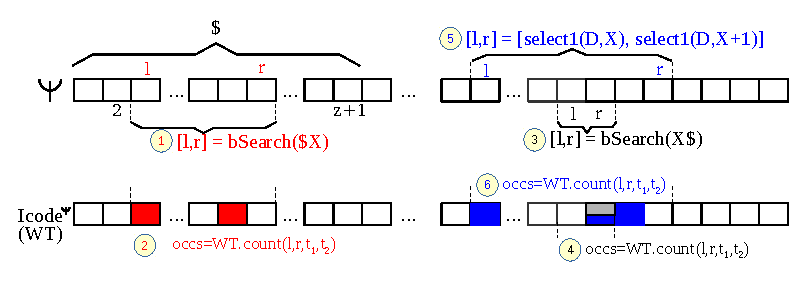
\includegraphics[width=0.90\textwidth]{figures/search2.eps}}
		\end{center}
		\caption{Trips staring at, ending at, or using node $X$  during time interval $[t_1..t_2]$.}
		\label{fig:ctr:search2}
	\end{figure}
		
		\item {\em Number of trips ending at node $X$ during the time interval $[t_1..t_2]$ (\endX$_T$). }
		As above, we initially perform the spatial query $[l..r]\leftarrow\bsearch(X\$)$ to 
		obtain the range in $\Psi[l..r]$ that corresponds to the pattern $X\$$ (trips ending at node $X$). Then, we use  $\cnt_{t_1,t_2}(Icode^{\Psi},l,r)$ operation to count how many of those trips match the temporal constraint. See steps \textcircled{3} and \textcircled{4} in Figure~\ref{fig:ctr:search2}.
		
		\item {\em Number of trips using node $X$ during the time interval $[t_1..t_2]$ (\loadX$_T$).}
		As in the corresponding spatial query, the range $\Psi[l..r]$  is obtained with two $\select_1$ operations on $D$.
		Finally, $\cnt_{t_1,t_2}(Icode^{\Psi},l,r)$ finds the occurrences within the time interval $[t_1..t_2]$, thus solving this query in $O(log|I|)$ time.
		See steps \textcircled{5} and \textcircled{6} in Figure~\ref{fig:ctr:search2}.


	\begin{figure}[th]
		\begin{center}
			{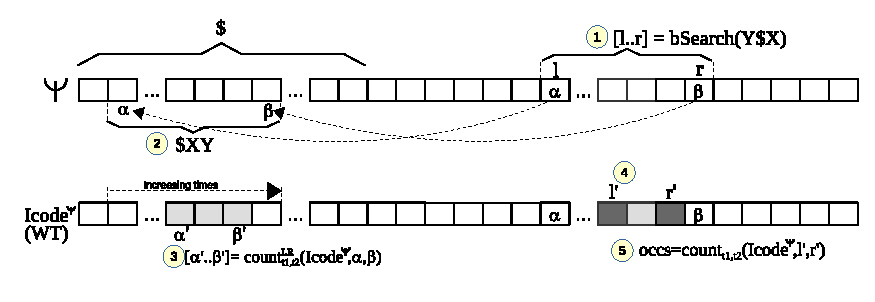
\includegraphics[width=0.90\textwidth]{figures/search.eps}}
		\end{center}
		\caption{Trips staring at $X$ and ending at $Y$ during time interval $[t_1..t_2]$.}
		\label{fig:ctr:search}
	\end{figure}
	
		\item {\em Number of trips starting at $X$ and ending at $Y$ occurring during  time interval $[t_1..t_2]$ (\XtoY$_T$).}
		We consider two different semantics. A query with  {\em strong semantics} will obtain trips
		that start and end within  $[t_1..t_2]$. Whereas, a query with  {\em weak semantics} will obtain trips whose time intervals overlap  $[t_1..t_2]$ and, therefore, they could actually start before $t_1$ or end after $t_2$.
		
		In Figure~\ref{fig:ctr:search}, we show the step-by-step process to solve this type of queries.
		As in a spatial query, we start by searching for the range $[l..r] \leftarrow \bsearch(\Psi,Y\$X)$ corresponding 
		to trips starting at $Y$ and ending at $X$ ({\em step-\textcircled{1}}). Next, due to our sorting of trips, the range for $Y\$X$ in $\Psi[l..r]$
		can be mapped to a continuous range $\Psi[\alpha..\beta]$ of the same size in the $\$X$ region of $\Psi$.\footnote{As the trips were sorted by the key $s_1,s_n,t_1,s_{2..n-1}$, and we positioned each $\$_i$ according to the order of their trip $\mathcal{T}_i$, the region $Y\$X$ will be conveniently sorted by the key $s_n,\$,s_1,s_n,t_1,s_{2..n-1}$ within $\Psi$, thus delimiting an equivalent region $\Psi[\alpha..\beta]$ in $\$X$ where each entry corresponds to a trip that also ends in $Y$.} 
		We compute $\alpha \leftarrow \Psi[l], 
		\beta\leftarrow\alpha+r-l$ ({\em step-\textcircled{2}}). Furthermore, note that the range for $\$XY$ preserves the same order as that for $Y\$X$.
		
		At this point, since $Icode^{\Psi}$  was aligned with $\Psi$, 
		we could check ending-time constraints within $Icode^{\Psi}[l..r]$  and starting-time constraints 
		within $Icode^{\Psi}[\alpha..\beta]$ (recall we keep starting times associated with the corresponding $\$$ of each trip).
		Note also that, due to our sorting (by starting-node, ending-node, starting-time,$\dots$) the times in $Icode^{\Psi}[\alpha..\beta]$ are 
		increasing ($Icode^{\Psi}[i] \leq Icode^{\Psi}[i+1], \forall \alpha \leq i < \beta$), as long as they are within the region $\Psi[\alpha..\beta]$, which corresponds to trips with the same starting-node $X$ and ending-node $Y$.
		Therefore, we can find the continuous subrange $[\alpha'..\beta'] \subseteq [\alpha..\beta] $ corresponding to trips
		that start within $[t_1..t_2]$ ({\em step-\textcircled{3}}).
		%We refer to this operation as $\cnt^{LR}$ in Figure~\ref{fig:ctr:search}.
		This operation was defined as $\cnt^{LR}_{a, b}(Icode^{\Psi},i,j)$ in Section~\ref{sec:wt}.
		Thus, that assuming $Icode^{\Psi}[\alpha..\beta]$ are increasing,  
		$[\alpha'..\beta'] \leftarrow \cnt^{LR}_{t_1,t_2}(Icode^{\Psi},\alpha,\beta)$ would report the 
		positions $[\alpha'..\beta'] \subseteq [\alpha..\beta]$ such that $\alpha' = argmin_{x} (Icode^{\Psi}[x] \geq t_1)$ and
		$\beta' = argmax_{x} (Icode^{\Psi}[x] \leq t_2)$.
		
		%Using a \gls{wt}, a simple way to implement $\cnt^{LR}$  consists in performing two binary searches within $[\alpha..\beta]$ to find $[\alpha'..\beta']$, where at each step we would use $\access$ operation. This would cost $O(\log n \log \sigma)$. 
		%Yet, we could also regard on $\cnt$ operation to obtain a more efficient and also rather straightforward implementation of $\cnt^{LR}$ so that we set $\alpha' \leftarrow count(\alpha,\beta,-1,t_1-1)$ and $\beta' \leftarrow \alpha'+ count(\alpha,\beta,t_1,t_2)$. It costs $O(\log\sigma)$.
		
		The last step will differ on whether the query is implementing strong or weak semantics:
		
		\begin{itemize} 
			\item {\em Strong semantics (\XtoY$_{Ts}$).} Note that the subrange $[\alpha'..\beta']$ (containing trips starting within $[t_1..t_2]$) 
			has a matching subrange $[l'..r'] = [l+\alpha'-\alpha..l+\beta'-\alpha] \subseteq [l..r]$ ({\em step-\textcircled{4}}), where some of the ending times of these trips will fall inside 
			$[t_1..t_2]$, allowing us to check the ending time constraint. By performing  $\cnt_{t_1,t_2}(Icode^{\Psi},l',r']$  we get the final result 
			({\em step-\textcircled{5}}). 
			To sum up, answering this query  requires: one $\bsearch$ over $\Psi$ (to find $[l..r]$), one $\access$ to $\Psi$ to obtain
			 $\alpha$ (since $\beta = \alpha+r-l$), one $\cnt^{LR}$ to find $[\alpha'..\beta']$, and one final $\cnt$ operation to count the valid ending times in $[l'..r']$, amounting in a total of $O(\log n + \log|I|)$ time.
			
			
			\item {\em Weak semantics (\XtoY$_{Tw}$).}
			The size of $[\alpha'..\beta']$ ($\beta' - \alpha' + 1$) is already a partial answer. To get the final result, we need to add 
			also the occurrences of those trips starting before $t_1$ that end at $t_1$ or later, which can only exist if $\alpha<\alpha'$. 
			To do so, we need to obtain $l'\leftarrow l+\alpha'-\alpha$ as done in \XtoY$_{Ts}$, and compute $\cnt_{t_1, |I|}(Icode^{\Psi},l,l'-1)$. This gives us the number of time instants in the range $[l..l')$ of  $Icode^{\Psi}$ that fall inside $[t_1..|I|]$. 
			That is, ending times equal or after $t_1$. Yet again, the time complexity for this query is $O(\log n + \log|I|)$.
		\end{itemize}
		
		


	\item {\em Top-k most used nodes during  time interval $[t_1..t_2]$ (\topK$_T$).}
	Both the sequential and binary-partition approaches discussed in Section~\ref{sec:ctr:alg:sq} can be easily extended to support this query. The idea is that, when we add a node either to the min-heap or the priority-queue
	respectively, we compute its frequency within time interval $[t_1..t_2]$ (using $\cnt$ operation) 
	rather than using its overall frequency.

	\begin{itemize}
		\item In the {\em sequential approach (\topK$_{Tseq}$)}, given a node whose corresponding range
		in $\Psi$ is $\Psi[l..r]$, we compute its frequency using $\cnt_{t_1,t_2}(Icode^{\Psi},l,r)$ instead of simply using  $r-l+1$. 
		The rest of the process is exactly as discussed for the pure spatial \topK$_{seq}$\ query. The time complexity is increased by a factor of $O(\log|I|)$ over the spatial \topK$_{seq}$\ variant, resulting in $O(|S|\log k\log|I|)$.
		
		\item In the {\em binary-partition approach (\topK$_{Tbin}$)}, we have to consider the priority of a
		given segment as the number of trips covered by that segment that occurred during $[t_1..t_2]$. Again, given
		a segment $[l..r]$ in $\Psi$ we compute that priority as $p_{l..r} \leftarrow \cnt_{t_1,t_2}(Icode^{\Psi},l,r)$ instead of 
		$p_{l..r} \leftarrow  r-l+1$. Apart from
		that, the only modifications that we must consider over the pure spatial \topK$_{bin}$\ Algorithm~\ref{alg:topk_nieves} are:
		we replace \textit{line 3} by $p_{l..r} \leftarrow \cnt_{t_1,t_2}(Icode^{\Psi},\select_1(D,2),n)$; $Q.push(\langle2, |V|\rangle, \langle \select_1(D,2), n\rangle, \underline{p_{l..r}})$,
		and we replace  \textit{lines 12 and 13}, respectively, by 
		   $ Q.push(\langle i, m-1 \rangle, \langle l, q-1 \rangle, \underline{\cnt_{t_1,t_2}(Icode^{\Psi},l,q-1)})$ and
		   $ Q.push(\langle m,   j \rangle, \langle q,   r \rangle, \underline{\cnt_{t_1,t_2}(Icode^{\Psi},q,r)})$. Due to these modifications, the overall time complexity for this variant is $O(|S|\log|S|\log|I|)$.
		
	\end{itemize}


	\item {\em Top-k most used nodes to start a trip during time interval $[t_1..t_2]$(\topK$_{Ts}$).}
	Following the same guidelines discussed above for \topK$_T$, adapting the  sequential and 
	binary-partition solutions for the spatial \topK$_s$\ to include temporal constraints is straightforward, making its time complexity $O(|S|\log|S|\log|I|\log n)$.
	\end{itemize}


\section{Experiments}
\label{sec:ctr:exp}
	We have run experiments to evaluate both the space requirements and performance at query time of \gls{ctr}
	when dealing with spatial, temporal, and spatio-temporal queries over two different datasets 
	(Porto and Madrid) that are described in Section~\ref{sec:ctr:exp:data}. 

	We have used several configurations of \gls{ctr} by tuning both its
	spatial and temporal components. In the spatial part, %(Section~\ref{sec:ctr:str:spat}), 
	we set the  $\Psi$ sampling parameter ($t_{\Psi}$) to the values $t_{\Psi} \in \{32, 128, 512\}$. 
	For the temporal component, % (Section~\ref{sec:ctr:str:temp}), 
	we have tested both the 
	balanced \gls{wm}, and the Hu-Tucker-shaped \gls{wt} (\gls{htwt}) using the bitvector configurations
	discussed in Section~\ref{sec:ctr:str:time:imp}. That is, using either a plain bitvector $RG$ with a 
	sparse sampling ($RG_{32}$), or a $RRR$ bitvector with sampling parameter $\in \{32,64,128\}$ 
	($RRR_{32}, RRR_{64}$, and $ RRR_{128})$.


	\subsection{Experimental datasets}
	\label{sec:ctr:exp:data}
	We used two different datasets of trips in our experiments:
	\begin{itemize}
	
	  \item {\bf Madrid dataset}:
	  Using \gls{gtfs} data obtained for the public transportation network of 
	  {Madrid},\footnote{Data from
	  the CRTM corporation at \url{http://www.crtm.es/}.} we generated a dataset of 
	  synthetic trips combining the subway network with the Spanish commuter rail system.\footnote{Data manually scraped from public sources.} (called {\em cercan\'ias})
	  In this dataset, we have defined the nodes as stops or stations, making two of them connected if there exists a line or route that stops at both nodes, consecutively, thus allowing us to represent user trajectories following the same strategy as for urban street networks.
	  In total, there are $313$ different stations/nodes from $23$ lines.
	 
	We generated $10$ million trips with lengths varying from $2$ to $31$ nodes traversed. Those lengths follow a binomial 
	distribution. The average length of the trips is $11.81$ nodes. 
	
	In the generation of a trip of length $l$, we randomly choose a starting node from a line, and the starting direction. 
	Then, we follow that line until we reach a switching node. At this node, we decide whether to follow the current 
	line or to switch to a new line. We allow only up to four line switches for a given trip, and use fixed probability 
	values to decide whether to switch line or not. Such probability is $0.5$, $0.1$, $0.05$, and $0.02$ respectively 
	for the first, second, third, and fourth line switch in a trip. 
	We also avoid revisiting nodes in the same trip. 
	The generation process ends when $l$ nodes have been added to the trip, or a dead end is reached.

	As a baseline, the plain representation of the generated trips using a $9$-bit integer ($\lceil\log_2 314\rceil= 9$) 
	for every node-ID (and the $\$$ separator) would require $137.47$ MiB, while requiring a sequential processing on the whole collection to answer most of our proposed queries.
	 
	We also generated synthetic times for those trips following the same rules used to create the time distribution
	named \textit{skewed} in Figure~\ref{fig:ctr:distrib}, so most of the trip timestamps belong to rush hours. 
	Instead of using only regular working days, we distinguished four kinds of days in a week:
	regular working days; Fridays and holiday eves; Saturdays; and Sundays and holidays. We also 
	assume that there are two kinds of weeks related to high and low season periods. 
	Therefore, a time interval may belong to eight types of day. 
	When discretized at five-minute intervals we obtain $2,\!304$ distinct time intervals, 
	while when we use thirty-minute intervals we obtain $384$. In the former case, our  baseline
	 for the generated times using  $12$ bits per time-ID would occupy $183.30$ MiB. In the latter one, each time-ID requires  $9$ bits and the  temporal baseline requires $137.47$ MiB.
	 
	 \begin{figure}[ht]
		\begin{center}
			\includegraphics[angle=-90,width=0.80\textwidth]{figures_synt/timedistrib.eps}		
			\caption{Time distributions tested. The final Madrid dataset was generated with the distribution called \textit{skewed}. The y-axis indicates the number of passengers per each 5-min interval.}
			\label{fig:ctr:distrib}
		\end{center}
	\end{figure}

	\item \textbf{Porto dataset}:
		We downloaded a collection of $1,\!710,\!671 $ trajectories from the city of {Porto} corresponding to taxi trips during 
		a full year (from July 1, 2013 to June 30, 2014), provided by \cite{moreira2013predicting}.\footnote{Description at \url{http://www.geolink.pt/ecmlpkdd2015-challenge/dataset.html} . Downloaded from \url{https://archive.ics.uci.edu/ml/machine-learning-databases/00339/train.csv.zip}} Among other
		fields those data include, for each taxi ride, a list of GPS coordinates and times gathered every $15$ seconds of
		the trip. We adapted such data to our needs by using a map matching algorithm provided by the Graphhopper library,\footnote{\url{https://github.com/graphhopper/map-matching}}
		 and OpenStreetMap cartography.\footnote{\url{http://www.openstreetmap.org/}} With this, we could determine what streets segments were traversed by the trips from their list of coordinates. Finally, trips were encoded as a sequence of identifiers
	  corresponding to adjacent stretches of street (that is, basic street segments with no intersections) the trip traversed, each one of them tagged with a timestamp.
	  
	  After filtering incomplete matches, $1,\!617,\!774$ trips, built  over $59,\!618$ distinct street segments, were used for the dataset. 
	  Due to the nature of the network and the trips, 
	  the average number of street segments per trip is $64.74$; that is, the length of the trips is longer than in Madrid dataset.
	  Since we needed $16=\lceil\log_2 59,\!618 \rceil$ bits to represent each segment in a trip, the total size of our plain spatial baseline is $202.85$ MiB.

	  For the temporal part, we considered only one kind of day. Therefore, when we sample those $24$ hours into five-minute intervals,
	  we obtain $288$ distinct time intervals that are given a $9$-bit time-ID. Consequently the overall size of the temporal
	  baseline becomes $114.10$ MiB. However, if we split those $24$ hours into thirty-minute intervals, only $48$ time intervals 
	  arise. In this case, each time-ID needs only $6$ bits and the total size of the temporal baseline is $76.07$ MiB.
	\end{itemize}


	\subsection{Space Requirements}
	\label{sec:ctr:exp:space}
	We show the compression obtained by \gls{ctr} when built on our two test datasets. Compression is shown as the percentage of the size of the plain baselines discussed above.
	Using different configurations of \gls{ctr}, we will show the compression of the spatial component (\gls{csa}), 
	that of the temporal component (\gls{htwt} and \gls{wm}), and finally the overall compression of \gls{ctr}.

	\begin{table}[ht]
	\begin{center}
	  \begin{tabular}{|l|*{3}{r}|}
	  \cline{2-4}
	  \multicolumn{1}{c|}{} & \multicolumn{3}{c|}{$t_{\Psi}$ } \\
	  \multicolumn{1}{c|}{} & 32 & 128 & 512 \\
	  \hline
	  Madrid & 41.32\% & 26.80\% & 23.06\% \\
	  Porto & 23.66\% & 15.49\% & 13.37\% \\
	  \hline
	  \end{tabular}
	  
	\caption{Compression of \acrshort{csa} with respect to the spatial baseline.}
	\label{table:ctr:exp:space:spat}
	\end{center}
	\end{table}

	Results regarding the compression obtained by \gls{csa} are given in Table~\ref{table:ctr:exp:space:spat}.
	The compression ratio is calculated over a plain spatial-only (stop-IDs or street-segment-IDs in each case) representation.
	Note that an $iCSA$  built on English text~\cite{FBNCPR12} typically
	reached the compression of {\em gzip} (around 35\% in compression ratio).
	As expected, the high compressibility of our sorted datasets of trips helps our \gls{csa} to improve those numbers with compression ratios under 30\%, while also offering indexing features
	that allow us to perform efficient searches.
	In a rather dense 
	configuration of \gls{csa} with $t_{\Psi}=32$ we obtain compression ratios around $41$\% and $23$\% for Madrid and Porto datasets respectively.
	Those results are interesting from the simple fact that the baseline representations were only using respectively 
	$9$-bits per node (Madrid) and $16$-bits per segment (Porto). 
	As expected, compression improves as we increase the $\Psi$ sampling parameter $t_{\Psi}$. We show that by tuning 
	\gls{csa} in a more sparse setup we can almost halve the space needs of using $t_{\Psi}=32$, although the resulting \gls{csa} would become
	much slower as we will later prove in Section~\ref{sec:ctr:exp:queries}.
	In general, we can see that \gls{csa} obtains better compression in Porto than in Madrid. This is probably due to the longer and
	more predictable trips. Note that is not common to arrive at an intersection having more than two valid street links where to navigate to.

	\begin{table}[ht]
	\begin{center}
	  \begin{tabular}{|l|*{4}{r}|}
	  \cline{2-5}
	  \multicolumn{1}{c|}{} & \multicolumn{4}{c|}{Type of bitvector in \gls{wm}/\gls{htwt}}\\

	  \multicolumn{1}{c|}{}   & $RG_{32}$& $RRR_{32}$& $RRR_{64}$& $RRR_{128}$\\
	  \hline                                             
	  Madrid (\gls{htwt}, 5-min) &  91.33\% &	 80.89\% &	 76.90\% & 	 74.90\% \\
	  Madrid (\gls{wm}, 5-min)   & 103.13\% &	 86.03\% &	 80.61\% & 	 77.88\% \\
	  Madrid (\gls{htwt}, 30-min)&  92.30\% &	 78.90\% &	 74.66\% &	 72.52\% \\
	  Madrid (\gls{wm}, 30-min)  & 103.14\% &	 83.32\% &	 77.90\% &	 75.18\% \\
	  \hline                  
	  Porto (\gls{htwt}, 5-min)  &  93.52\% &	102.61\% &	 98.27\% &	 96.11\% \\
	  Porto (\gls{wm}, 5-min)    & 103.13\% &	106.88\% &	101.41\% &	 98.66\% \\
	  Porto (\gls{htwt}, 30-min) &  96.00\% &	103.78\% &	 99.08\% &	 96.74\% \\
	  Porto (\gls{wm}, 30-min)   & 103.12\% &	107.00\% &	101.50\% &	 98.75\% \\

	  \hline
	  \cline{2-5}
	  \end{tabular}
	\end{center}
	
	\caption{Compression of \acrshort{wm} and \acrshort{htwt} with respect to the temporal baseline.}
	\label{table:ctr:exp:space:wt}
	\end{table}

    \medskip
	In Table~\ref{table:ctr:exp:space:wt}, we focus on the space needed by the temporal component of \gls{ctr}. 
	In this case we show the compression ratios obtained by \gls{htwt} and \gls{wm} 
	considering that time is either discretized into $5$-min or $30$-min intervals. Recall that the size of the 
	plain baseline representations differs depending on the discretization period. Both \gls{htwt} and \gls{wm} were tuned by
	using bitvector representations $RG_{32}$, $RRR_{32}$, $RRR_{64}$, and $ RRR_{128}$, as indicated above.

	One important insight from these results is that in the synthetic dataset from Madrid $RRR$ bitvectors always lead to a better compression than the plain $RG$, while in the real dataset from Porto that is not always the case, and we have to use the sparsest configuration of $RRR$ to achieve similar space requirements of the uncompressed $RG$ version. Consequently, for Porto dataset, the faster plain $RG$ bitvectors are probably the best choice. In Madrid dataset, we can see an actual space/time trade-off: $RRR$ obtains better compression but will be slower, as later seen in Section~\ref{sec:ctr:exp:queries}.

	\begin{table}[ht]
	
	\begin{center}
	  \begin{tabular}{|c|l|*{4}{c}|}
	  \cline{3-6}
	  \multicolumn{2}{c|}{} & \multicolumn{4}{c|}{Type of bitvector in \gls{wm}/\gls{htwt}} \\

	  \multicolumn{2}{c|}{}     &$RG_{32}$& $RRR_{32}$& $RRR_{64}$&$RRR_{128}$ \\
	  \hline
	  \multirow{8}{*}{\STAB{\rotatebox[origin=c]{90}{$t_{\Psi}=32$}}}
	   & Madrid (\gls{htwt}, 5-min)  & 69.90\% &   63.93\% &   61.65\% &   60.51\% \\
	   & Madrid (\gls{wm}, 5-min)     & 76.64\% &   66.87\% &   63.77\% &   62.21\% \\
	   & Madrid (\gls{htwt}, 30-min) & 66.81\% &   60.11\% &   57.99\% &   56.92\% \\
	   & Madrid (\gls{wm}, 30-min)    & 72.23\% &   62.32\% &   59.61\% &   58.25\% \\
	  \cline{2-6}
	   & Porto (\gls{htwt}, 5-min)   & 48.81\% &   52.08\% &   50.52\% &   49.74\% \\
	   & Porto (\gls{wm}, 5-min)      & 52.27\% &   53.62\% &   51.65\% &   50.66\% \\
	   & Porto (\gls{htwt}, 30-min)  & 43.39\% &   45.51\% &   44.23\% &   43.59\% \\
	   & Porto (\gls{wm}, 30-min)     & 45.33\% &   46.39\% &   44.89\% &   44.14\% \\
	  \hline
	  %\cline{2-5}
	  %\multicolumn{1}{c|}{} & \multicolumn{4}{c|}{$t_{\Psi}=32$} \\
	%	\cline{2-5}
	 % \end{tabular}
	  
	  %\begin{tabular}{|l|*{4}{c}|}
	  %\cline{2-5}
	  %\multicolumn{1}{c|}{} & \multicolumn{4}{c|}{Type of bitvector in \gls{wm}/\gls{htwt}} \\

	  %\multicolumn{1}{c|}{}     &$RG_{32}$& $RRR_{32}$& $RRR_{64}$&$RRR_{128}$ \\
	  \multicolumn{5}{c}{} \\
	  \hline   
	  \multirow{8}{*}{\STAB{\rotatebox[origin=c]{90}{$t_{\Psi}=512$}}}
	   & Madrid (\gls{htwt}, 5-min) & 62.07\% &	56.10\% &	53.82\% &	 52.68\% \\
	   & Madrid (\gls{wm}, 5-min)   & 68.81\% &	59.04\% &	55.94\% &	 54.38\% \\
	   & Madrid (\gls{htwt}, 30-min) &  57.68\% &	50.98\% &	48.86\% &	 47.79\% \\
	   & Madrid (\gls{wm}, 30-min)  & 63.10\% &	53.19\% &	50.48\% &	 49.12\% \\
	  \cline{2-6}
	   & Porto (\gls{htwt}, 5-min)   & 42.22\% &	45.49\% &	43.93\% &	 43.15\% \\
	   & Porto (\gls{wm}, 5-min)      & 45.68\% &	47.03\% &	45.06\% &	 44.07\% \\
	   & Porto (\gls{htwt}, 30-min)  & 35.91\% &	38.03\% &	36.75\% &	 36.11\% \\
	   & Porto (\gls{wm}, 30-min)   & 37.85\% &	38.91\% &	37.41\% &	 36.66\% \\
	  \hline
	  %\cline{2-5}
	  %\multicolumn{1}{c|}{} & \multicolumn{4}{c|}{$t_{\Psi}=512$} \\
	%	\cline{2-5}
	  \end{tabular}
	\end{center}
	
	\caption{Overall compression of \acrshort{ctr} including different configurations for both the spatial and temporal components.}
	\label{table:ctr:exp:space:ctr}
	\end{table}


    \medskip
	Finally, in Table~\ref{table:ctr:exp:space:ctr}, we show the overall compression rates of  \gls{ctr}.
	We use the same configurations for \gls{htwt} and \gls{wm}  as in Table~\ref{table:ctr:exp:space:wt}, and both the
	most dense and sparse tuning of \gls{csa} ($t_{\Psi}= 32$ and $t_{\Psi}= 512$ respectively).
	For Madrid dataset, the pair \mbox{(node, timestamp)} is represented with $9+9=18$ bits in our baseline representation 
	when time is discretized into $30$-minute intervals, and with $9+12=21$ when we use $5$-minute intervals.
	In the case of Porto dataset, when using $30$-minute intervals, each pair \mbox{(node, timestamp)} from the baseline requires $16+9=25$ bits. 
	If discretization considers $5$-minute intervals, the baseline requires $16+6=22$ bits. We can see that the overall
	compression of \gls{ctr} in Madrid dataset ranges between $76\%$ and $50\%$. Also we show that Porto dataset is much
	more compressible, obtaining compression ratios from around $50\%$ down to $35\%$.


	%%%%%%%%%%% DESCOMENTAR CUANDO FARI CAMBIE DE OPINION %%%%%%%%%%%

	% \begin{table}[h!]
	% %\vspace{-6mm}
	% \begin{center}
	% \scriptsize
	%   \begin{tabular}{l*{4}{c}|*{4}{c}|r|}
	%   %\hline
	%   & \multicolumn{4}{c}{Hu-Tucker \gls{wt}} & \multicolumn{4}{c}{\gls{wm}} & \multicolumn{1}{r}{} \\
	%   \cline{2-9}
	%   & RG32 & RRR32 & RRR64 & RRR128 & RG32 & RRR32 & RRR64 & \multicolumn{1}{c}{RRR128} & \multicolumn{1}{r}{} \\ \hline

	%   X To Y (s) & RG32 & RRR32 & RRR64 & RRR128 & RG32 & RRR32 & RRR64 & RRR128 & \multirow{7}{*}{\rotatebox{270}{5 minutes}} \\
	%   X To Y (s) & RG32 & RRR32 & RRR64 & RRR128 & RG32 & RRR32 & RRR64 & RRR128 & \\
	%   X To Y (s) & RG32 & RRR32 & RRR64 & RRR128 & RG32 & RRR32 & RRR64 & RRR128 & \\
	%   X To Y (s) & RG32 & RRR32 & RRR64 & RRR128 & RG32 & RRR32 & RRR64 & RRR128 & \\
	%   X To Y (s) & RG32 & RRR32 & RRR64 & RRR128 & RG32 & RRR32 & RRR64 & RRR128 & \\
	%   X To Y (s) & RG32 & RRR32 & RRR64 & RRR128 & RG32 & RRR32 & RRR64 & RRR128 & \\
	%   Starts In X & RG32 & RRR32 & RRR64 & RRR128 & RG32 & RRR32 & RRR64 & RRR128 & \\ \hline

	%   \end{tabular}
	% %\vspace{-5mm}
	% \caption{Test table}
	% \label{table:madrid}
	% %\vspace{-10mm}
	% \end{center}
	% \end{table}




	\subsection{Performance at query time}
	\label{sec:ctr:exp:queries}
	Through this section, we evaluate the time performance of \gls{ctr} when solving spatial, temporal, and spatio-temporal queries.
	We have randomly generated $10,\!000$ query patterns from our two datasets for each type of query.
	Each time measurement presented below is the average execution time of $10,\!000$ runs using the corresponding query patterns, 
	except for the \topK\ queries where we perform $100$ runs of the {\em top-k} algorithms with $k\in\{10,100\}$.

	Our test machine has an Intel(R) Core(tm) i5-4690@3.50GHz CPU (4 cores/4 siblings) and 8GB of DDR3 RAM. 
	It runs Ubuntu Linux 16.04 (Kernel 4.4.0-21-generic). The compiler used was GCC version 5.4.0 and we set compiler optimization flags to $-O3$. All our experiments run in a single core and time measures refer to CPU user-time.

	During the generation of query patterns, for those queries involving only one node $X$ from the network, 
	we have randomly chosen $X$ $10,\!000$ times from the available network nodes. 
	This is the case of the query patters used both for
	the spatial queries \startX, \endX, and \loadX\ or the spatio-temporal \startX$_T$, \endX$_T$, and \loadX$_T$.
	In the case of the spatial \XtoY\ and the spatio-temporal \XtoY$_{Ts}$, and \XtoY$_{Tw}$\ the pair of
	network nodes $\langle X,Y \rangle$ that compose our
	query patterns were generated by randomly choosing
	$10,\!000$ trips and then extracting the initial $X$ and ending $Y$ nodes of those trips, in order to avoid generating queries for pairs $\langle X,Y \rangle$ that were absent in our dataset.

	Moreover, we also generated the time intervals $[t_1..t_2]$ required for 
	the spatio-temporal queries. Considering the different available time-IDs, we chose a random starting
	instant $t_1$ and then randomly generated the width of that interval from five minutes to two hours.
	Note that if we discretized time into $5$-minute intervals and $interval$-$width=59$ minutes, our time
	interval $[t_1..t_2]$ would contain exactly $12$ time IDs ($t_2\leftarrow t_1+11$). However, if time was
	discretized into $30$-minute intervals, $[t_1..t_2]$ would contain only $2$ time IDs ($t_2\leftarrow t_1+1$).
	We followed the same procedure to generate the query patterns used for the pure temporal queries \loadT\ and \startT.

	\subsubsection{Space/time trade-off when dealing with spatial queries} \label{sec:ctr:exp:queries:spat}

	In Figures~\ref{fig:ctr:exp:queries:spat:madrid} and \ref{fig:ctr:exp:queries:spat:porto}, we show the performance of \gls{ctr} at
	solving spatial queries for Madrid and Porto datasets respectively. 
	Note that all these queries can be answered using only the \gls{csa} component
	of \gls{ctr}. Therefore, the size of the temporal component 
	is not considered here and compression values (x-axis) refer only to the size of \gls{csa} with
	respect to the spatial baseline as in Table~\ref{table:ctr:exp:space:spat}. 
	We show the average query time (in $\mu$s) depending on the
	space used by \gls{csa} with three different 
	sampling configurations ($t_{\Psi} \in \{512, 128, 32\}$).

	Results show that the queries that involve searching in the $\$$ region of 
	$\Psi$, such as \startX\ or \XtoY\ are considerably slower than queries \endX\ and \loadX\ 
	due to the large size of that region when compared to the frequency of any node: in neither of the two datasets there is a node that was visited by every trip, while there is one $\$$ per trip.

	\begin{figure}[ht]
		\begin{center}
			{\includegraphics[angle=-90,width=0.45\textwidth]{figures_synt/madrid_spatial.eps}}
			{\includegraphics[angle=-90,width=0.45\textwidth]{figures_synt/madrid_spatial_topk.eps}}
		\end{center}
		\caption{Spatial queries (left) and spatial {\em top-k} queries (right) for Madrid.}
		\label{fig:ctr:exp:queries:spat:madrid}
	%\end{figure}

	%\begin{figure}[ht]
		\begin{center}
			{\includegraphics[angle=-90,width=0.45\textwidth]{figures_synt/porto_spatial.eps}}
			{\includegraphics[angle=-90,width=0.45\textwidth]{figures_synt/porto_spatial_topk.eps}}
		\end{center}
		\caption{Spatial queries (left) and spatial {\em top-k} queries (right) for Porto.}
		\label{fig:ctr:exp:queries:spat:porto}
	\end{figure}

	In both datasets, we can see that \loadX\ (solved using $\select$ on $D$ rather than
	$\bsearch$ on $\Psi$) is the fastest query. On average, it takes only around $10$ns
	per query. Except in the most sparse configuration of \gls{csa}, queries \endX, \startX, and 
	\XtoY\ require typically less than $10\mu$s. This basically shows the cost of performing
	$\bsearch$ on a compressed $\Psi$. In the most sparse setup ($t_{\Psi}=512$), times for \startX\ and \XtoY\ are always better 
	for the dataset of Madrid than for the one of Porto, and \endX\ draws rather identical times.
	With the densest configuration  ($t_{\Psi}=32$), \endX\ and \XtoY\ are respectively 
	around $10$-$20$\% fastest in Madrid dataset (\endX\ takes $4.05\mu$s and $4.51\mu$s respectively, and
	\XtoY\ takes $4.54\mu$s and $5.66\mu$s). However, \startX\ performs around $20$\% faster in Porto dataset 
	($2.28\mu$s vs $2.90\mu$s).
	\medskip

	Focusing on \topK\ queries, we can see huge differences between \topK$_s$\  
	and the rest of the \topK\ queries, as the former needs to perform {$ \bsearch$} over the compressed $\Psi$
	instead of a $\select$ on $D$. 

	We can also see that due to the small number of stops in Madrid dataset, it is always more efficient to use the sequential version of \topK$_s$\ and \topK\ algorithms. This is also because a rather uniform frequency among nodes 
	increases the number of insertions in the priority queue ($i$) of the \mbox{binary-partition} algorithm
	needed for retrieving the first $k$ nodes ($i \approx |S|$). Moreover, note that for the sequential algorithm $i$ is at most $|S|$, whereas for the binary-partition counterpart it could become up to $2|S|-1$.

	However, in Porto dataset, where nodes follow a biased distribution (some streets are much more used than others by taxis), and a vocabulary 
	is $190$ times larger than the one for Madrid, the binary-partition version of \topK$_s$\ and \topK\ algorithms is clearly
	faster than the sequential counterpart (\topK$_{seq}$\ and \topK$_{sseq}$).
	Note that in Madrid dataset, $top\_100$ returns 32\% of the nodes (hence sequential processing worths it) 
	whereas in Porto dataset less than 0.2\% of the nodes are returned. 

	The gap between $top\_10_{seq}$ and $top\_100_{seq}$ that we can clearly appreciate in Madrid dataset 
	is due to the cost of the insertion of nodes in the min-heap. However, the gap between 
	the binary $top\_10_{bin}$ and $top\_100_{bin}$ 
	is mainly related to the number of iterations performed until the binary-partition algorithm gathers the first
	$10$ and $100$ {nodes}  returned respectively. The same discussion applies for \topK$_s$\ queries.


	\subsubsection{Comparing the space/time trade-off of WM and HTWT}
	\label{sec:ctr:exp:queries:wt}
	In order to compare the efficiency of our \gls{htwt} (that uses variable-length codes and supports $\cnt$ efficiently) with a balanced \gls{wm} alternative under 
	different time distributions (recall that this \gls{wm} is time distribution invariant), 
	we run some experiments that evaluate the average time to execute $\cnt$ operation on
	both representations.

	We used a dataset of generated trips for Madrid (refer to Section~\ref{sec:ctr:exp:data} for details) and we
	generated three kinds of time distributions for our evaluation. We refer to them as: uniform, skewed, and very skewed, as they are shown
	in Figure~\ref{fig:ctr:distrib}. 
	According to the total number of passengers in a day, in the uniform distribution, $51,\!000$ passengers 
	use the network for each 5-minute interval. 
	We also generated a skewed distribution for the time interval frequencies in an effort to
	model the usage of a public transportation network in a regular working day, where the starting time of a trip
	is generated according to the following rules:
	%
	\begin{itemize}
		\item With 30\% of probability, a trip occurs during a morning rush hour.
		\item With 45\% of probability, a trip occurs in an evening rush hour.
		\item With 5\% of probability, a trip occurs during lunch rush hour.
		\item The remaining 20\% of probability is associated to unclassified trips, starting at a random hour of the day, which may also fall into one of the three previous periods discussed.
	\end{itemize}
	%
	In the very skewed distribution we increase the rush-hour probabilities with
	40\% for the morning rush hour, 50\% for the evening rush hour, 8\% for lunch period and only
	2\% of random movements.
	\medskip

	For these generated datasets, we have built the \gls{htwt} and the \gls{wm} considering two different granularities for the discretization of times: 
	five-minute and thirty-minute intervals. Then, we generated $10,\!000$ random intervals of times $[t_1..t_2]$ over the whole 
	time sequence of the dataset considering interval widths of five minutes, one hour, and six hours.  
	Finally, we run $10,\!000$  $\cnt_{t_1,t_2}(Icode^{\Psi},|\mathcal{T}|+2,n)$ queries (we show average times) from each query set over 
	the six configurations of \gls{htwt} and \gls{wm}  
	(2 different granularities for the time discretization and 3 datasets).

	%We made a custom \gls{wt} implementation with Hu-Tucker coding, where we focused in optimizing the $\cnt$ operation. We also implemented the $top-k$ mentioned in Section~\ref{sec:ctr:alg:tq} using a binary partition approach.

	%For the \gls{wm} we reuse the implementation from \cite{CNO15}, with $top-k$ implemented with a simple linear approach, using leaf pointers that were already stored in the structure. That allows us to analyze the advantage of the linear when the distribution is uniform

	\begin{figure}[ht]
		\begin{center}
			\includegraphics[angle=-90,width=0.45\textwidth]{figures_synt/unif5m.eps}
			\includegraphics[angle=-90,width=0.45\textwidth]{figures_synt/unif30m.eps}
			\includegraphics[angle=-90,width=0.45\textwidth]{figures_synt/skewed5m.eps}
			\includegraphics[angle=-90,width=0.45\textwidth]{figures_synt/skewed30m.eps}
			\includegraphics[angle=-90,width=0.45\textwidth]{figures_synt/veryskewed5m.eps}
			\includegraphics[angle=-90,width=0.45\textwidth]{figures_synt/veryskewed30m.eps}
			\caption{Space/time trade-offs for {\em count} queries depending on the time distribution: 
				uniform (top), skewed (middle), and very skewed (bottom).
				Time granularity for the time index is 5 minutes (left) or 30 minutes (right).
			}
			\label{fig:ctr:exp:queries:wt:study}
		\end{center}
	\end{figure}

	In Figure~\ref{fig:ctr:exp:queries:wt:study}, we show the results of our experiments. In the upper part of the figure, we 
	include the results for \gls{htwt} and \gls{wm} built over the times assuming uniform frequency distribution.
	In the middle part we assume times follow a the skewed distribution, and in the bottom of the figure we show
	results when considering a very skewed distribution. Moreover, figures in the left column show results
	for our structures considering that a 5-minute granularity is chosen for the discretization of times, whereas
	figures on the right column assume time granularity is 30 minutes. For each scenario we include plots
	\texttt{wtht:5-min}, \texttt{wtht:1-hour}, and \texttt{wtht:6-hour} for \gls{htwt} (range width for $\cnt$ is respectively
	5-minutes, 1-hour, and 6-hours). We also present those plots for \gls{wm} (\texttt{wm:5-min}, \texttt{wm:1-hour}, and \texttt{wm:6-hour}).

	The baseline used for the space usage (x-axis) is the size of an array of
	fixed-length time-interval IDs represented with the least number of bits needed (12 bits and 9 bits
	respectively for 5-minute and 30-minute granularity, see Section~\ref{sec:ctr:exp:data}).
	\medskip

	When times are uniformly distributed, our \gls{htwt} can only exploit the redundancy introduced by
	the $\$$ symbols. With this, \gls{htwt} can obtain only a minimal compression (around $96-98\%$ of the baseline)
	when using a $RG$ (plain) bitvector, whereas \gls{wm} uses more space than the baseline (around $104\%$).
	Recall that, for each plot, we present four points corresponding (left-to-right) 
	to $RRR_{128}$, $RRR_{64}$, $RRR_{32}$, and $RG$ bitvectors.
	When using compressed  bitvectors ($RRR$), \gls{wm} becomes the best choice. It is both more compact 
	(bitvectors in \gls{wm} are more compressible) and faster than \gls{htwt}. 
	In any case, using $RRR$ clearly slows down queries.

	A skewed distribution favors the compression for a statistical coder like Hu-Tucker,
	which explains the higher compression obtained. However,
	it also slightly increases the query times, especially in the wider
	one-hour and six-hours query sets. This happens because the probability of having a query 
	that forces to descend completely up to the leaves of the \gls{htwt} also increases.

	For a very skewed distribution, the gap in compression between \gls{htwt} and \gls{wm} increases clearly (around 
	$5$ percentage points), whereas query times remain similar to those in the previous scenario.

	%In case of a \gls{wm} representation, the time and space efficiency is the same
	%regardless of the statistical distribution of the times in the dataset, as no
	%statistical coder has been used. As expected, in Figure~\ref{fig:ctr:exp:queries:wt:study}
	%the version with the plain bitvector {\em RG} uses even more space than the original unindexed
	%representation, as the bitvectors need additional structures for
	%$\rank$ and $\select$.
	%
	%Regarding query times, there is a slight advantage of the \gls{wm} that is mostly
	%because the Hu-Tucker codes are longer than the original binary codes in some cases,
	%increasing the height of the \gls{wt}. As we query random time intervals, a slightly
	%deeper level was reached for the \gls{wt} than for the \gls{wm} for some of the queries.


	As a conclusion of the experiments discussed in this section, we have shown that
	the distribution of the sequence of times can be
	exploited by our \gls{htwt} to achieve a better compression and even improved
	query times than the balanced \gls{wm} counterpart.


	% % % % % % % % % % % % % % % % % % % % % % % % % % % % % % % % % % % % % % % % % % % % % % % % % % % % % % %
	% % % % % % % % % % % % % % % % % % % % % % % % % % % % % % % % % % % % % % % % % % % % % % % % % % % % % % %
	\subsubsection{Space/time trade-off when dealing with temporal  queries}
	\label{sec:ctr:exp:queries:temp}
	% % % % % % % % % % % % % % % % % % % % % % % % % % % % % % % % % % % % % % % % % % % % % % % % % % % % % % %
	% % % % % % % % % % % % % % % % % % % % % % % % % % % % % % % % % % % % % % % % % % % % % % % % % % % % % % %

	In this section we focus on the performance of the temporal component of \gls{ctr}. We use the same 
	configurations as in Table~\ref{table:ctr:exp:space:wt} for \gls{wm} and \gls{htwt} (although we are only using generated times for Madrid following the \textit{skewed} variant, as previously stated in Section~\ref{sec:ctr:exp:data}), and 
	show the space/time trade-offs obtained when solving pure temporal queries. Figures~\ref{fig:ctr:exp:queries:temp:madrid}
	and \ref{fig:ctr:exp:queries:temp:porto} present the results obtained at  \loadT\ and \startT\ queries for Madrid and Porto datasets respectively. 
	Note that, in this case, since the \gls{csa} is not actually needed to solve temporal queries, we do not include its size
	within the compression values (x-axis). 

	% We can see that when running \Ttk\ queries, the uneven distribution of times that we generated for Madrid dataset 
	% clearly favors the binary-partition approach with respect to the sequential counterpart. Note that this happens 
	% even in \Ttcien\ where the number of time-IDs returned is very high with respect to the total existing time-IDs.
	% Having a wider $30$-min time interval reduces the height of \gls{htwt} and \gls{wm} (and the average number of
	% time-IDs involved), and consequently the query times. 
	% 
	% For Porto dataset we obtain similar results. Its real distribution of times is also biased and binary \Ttk\ are
	% still preferred.  Note that in this dataset, when time is discretized into $30$-min intervals we run
	% \Ttcuarenta\ instead of \Ttcien\ since there are only $48$ available time-IDs.
	% 
	% Regarding query \loadT\  we can see that both \gls{htwt} and \gls{wm} obtain similar times (requiring less than 4$\mu$s 
	% to perform a $\cnt$ operation) and that those times improve as the height of the structure decreases.
	% 
	% %When querying the top ten most used time intervals, we are using a sequential algorithm for the \gls{wm}, and binary 
	% %for the \gls{wt}. For this reason, in Figure~\ref{fig:ctr:exp:queries:temp:madrid} the points for each temporal index belong 
	% %to a completely different time range. The uneven distribution of times favors the binary algorithm of the \gls{wt}, 
	% %and having a wider time interval reduces the height of the \gls{wt} or the \gls{wm}.
	% %\OJOFARI{{\em pure temporal. Antes de enviar paper Daniil va a implementar top-k-binario en WM y top-k-secuencial en WTHT.
	% %	 	Cuando corra estos experimentos, se incluirán 2 nuevos plots en las figuras. 
	% %		Lo digo porque por ahora, top-k en WM es sequential, y en WTHT es binario.
	% %	}}




	%%%%%%%%%%% MADRID - PURE-TEMPORAL %%%%%%%%%%%%%

	\begin{figure}[ht]
		\begin{center}
			\begin{center}
				{\includegraphics[angle=-90,width=0.4\textwidth]{figures_synt/madrid_t5mht.eps}}
				{\includegraphics[angle=-90,width=0.4\textwidth]{figures_synt/madrid_t5mwm.eps}}
				{\includegraphics[angle=-90,width=0.4\textwidth]{figures_synt/madrid_t30mht.eps}}
				{\includegraphics[angle=-90,width=0.4\textwidth]{figures_synt/madrid_t30mwm.eps}}
			\end{center}
		\end{center}
		\caption{Pure temporal queries for Madrid, using either a \acrshort{htwt} (left) or a \acrshort{wm} (right). 
			Time granularity is $5$ minutes (top) or $30$ minutes (bottom).}
		\label{fig:ctr:exp:queries:temp:madrid}
	\end{figure}


	%%%%%%%%%%% PORTO - PURE TEMPORAL %%%%%%%%%%%%%


	\begin{figure}[ht]
		\begin{center}
				{\includegraphics[angle=-90,width=0.4\textwidth]{figures_synt/porto_t5mht.eps}}
				{\includegraphics[angle=-90,width=0.4\textwidth]{figures_synt/porto_t5mwm.eps}}
				{\includegraphics[angle=-90,width=0.4\textwidth]{figures_synt/porto_t30mht.eps}}
				{\includegraphics[angle=-90,width=0.4\textwidth]{figures_synt/porto_t30mwm.eps}}
		\end{center}
		\caption{Pure temporal queries for Porto, using either a \acrshort{htwt} (left) or a \acrshort{wm} (right). 
			Time granularity is $5$ minutes (top) or $30$ minutes (bottom).}
		\label{fig:ctr:exp:queries:temp:porto}
	\end{figure}



	We can see that when running \loadT\ queries, both \gls{htwt} and \gls{wm} obtain rather similar times (requiring less than 4$\mu$s 
	to perform a $\cnt$ operation in all cases) and that those times improve as the height of the structure decreases. We can see 
	that in the highest \gls{htwt} and \gls{wm}, corresponding to using $5$-min intervals in Madrid dataset, \loadT\ requires less
	than $3.5\mu$s. Then, when using $30$-min intervals, the time required to solve \loadT\ is always below $2.3\mu$s (yet
	\gls{wm} performs faster than \gls{htwt} here), and those times are similar to the ones obtained for Porto dataset when
	using $5$-min intervals. Finally, the best query times (below $1.2\mu$s) are obtained for Porto dataset with 
	$30$-min intervals.

	Regarding $\startT$, recall that it also performs a $\cnt$ operation, but within a smaller range ($[2..|\mathcal{T}+1|]$) in comparison with the range
	$[|\mathcal{T}|+2..n]$ where  $\cnt$ is performed for \loadT. We can see that, whereas the \gls{wm} obtains similar times to those of 
	$\loadT$ query,  \startT\ performs clearly faster than \loadT\ over the \gls{htwt}.
	
	While query times are bounded by $O(\log|I|)$, as seen in Section~\ref{sec:ctr:alg:tq}, it is observed that, in some cases, \startT\ is answered considerably faster than \loadT. This occurs because, for some of our randomly queried time intervals (of up to two hours), there are no trips starting around that queried time, allowing the $\cnt$ operation to be cut short before reaching the leaves of the \gls{htwt} or the last level of the \gls{wm}. The difference is obviously accentuated in the case of \gls{htwt}, as the tree is not uniform.


	%Due to the smaller vocabulary of times, in Porto dataset, we can see that all the indexes performs better for the top-10 times 
	%query in Figure~\ref{fig:ctr:exp:queries:temp:porto}, although the binary version of the \gls{wt} is still faster because the time 
	%distribution is not uniform either.


	As a final note, recall that in Madrid dataset, bitvector $RG$ always needs more space than $RRR$ counterparts 
	whereas in Porto dataset (as discussed in Section~\ref{sec:ctr:exp:space})
	$RG$ obtains the best space values when using $5$-min intervals and still requires less space than $RRR_{32}$ when using
	$30$-min intervals. 
	This is the reason why while plots for Madrid dataset are decreasing from left to right, in Porto
	dataset the first point ($RG$) in the left figures ($5$-min intervals), and the third point ($RG$) 
	in the right figures ($30$-min intervals) require less space than the others ($RRR$) and are also typically  faster. 
	%This is mainly noticeable for queries \XtoY$_{Ts}$\ and \XtoY$_{Tw}$.


	% % % % % % % % % % % % % % % % % % % % % % % % % % % % % % % % % % % % % % % % % % % % % % % % % % % % % % %
	% % % % % % % % % % % % % % % % % % % % % % % % % % % % % % % % % % % % % % % % % % % % % % % % % % % % % % %
	\subsubsection{Space/time trade-off when dealing with spatio-temporal queries}
	\label{sec:ctr:exp:queries:st}
	% % % % % % % % % % % % % % % % % % % % % % % % % % % % % % % % % % % % % % % % % % % % % % % % % % % % % % %
	% % % % % % % % % % % % % % % % % % % % % % % % % % % % % % % % % % % % % % % % % % % % % % % % % % % % % % %

	In Figures~\ref{fig:ctr:exp:queries:st:madrid} and \ref{fig:ctr:exp:queries:st:porto}, we show the space/time tradeoff obtained by \gls{ctr}\ when 
	dealing with spatio-temporal queries. Recall that this type of queries require both using the \gls{csa}, to 
	exploit indexed access to the nodes in the trips, and the 
	temporal component of \gls{ctr} to handle temporal constraints. In this case, the space values showed in
	the figures include both the size of \gls{csa} and that of either \gls{wm} or \gls{htwt}. Therefore, we also show the
	overall space needs of \gls{ctr}. In the case of \gls{csa} we
	have set $t_{\Psi}=32$ (a fixed dense sampling), and for \gls{wm} and \gls{htwt} we used again the same configurations as in the previous sections obtained by varying the bitvectors and the temporal discretization. 

	%%%%%%%%%%% MADRID -SPATIO-TEMPORAL %%%%%%%%%%%%%
	\begin{figure}[ht]
		\begin{center}
			{\includegraphics[angle=-90,width=0.4\textwidth]{figures_synt/madrid_ht5.eps}}
			{\includegraphics[angle=-90,width=0.4\textwidth]{figures_synt/madrid_wm5.eps}}
			{\includegraphics[angle=-90,width=0.4\textwidth]{figures_synt/madrid_ht30.eps}}
			{\includegraphics[angle=-90,width=0.4\textwidth]{figures_synt/madrid_wm30.eps}}
		\end{center}
		\caption{Spatio-temporal queries for Madrid, using either a \acrshort{htwt} (left) or a \acrshort{wm} (right). 
			Time granularity is $5$ (top) or $30$ minutes (bottom). 
		}
		\label{fig:ctr:exp:queries:st:madrid}
	\end{figure}


	%%%%%%%%%%% PORTO - SPATIO-TEMPORAL %%%%%%%%%%%%%

	\begin{figure}[ht]
		\begin{center}
			{\includegraphics[angle=-90,width=0.4\textwidth]{figures_synt/porto_ht5.eps}}
			{\includegraphics[angle=-90,width=0.4\textwidth]{figures_synt/porto_wm5.eps}}
			{\includegraphics[angle=-90,width=0.4\textwidth]{figures_synt/porto_ht30.eps}}
			{\includegraphics[angle=-90,width=0.4\textwidth]{figures_synt/porto_wm30.eps}}
		\end{center}
		\caption{Spatio-temporal queries for Porto, using either a \acrshort{htwt} (left) or a \acrshort{wm} (right). 
			Time granularity is $5$ (top) or $30$ minutes (bottom). 
		}
		\label{fig:ctr:exp:queries:st:porto}
	\end{figure}


	For queries \startX$_T$, \endX$_T$, and \loadX$_T$\ we can see typically small differences between using \gls{wm} or \gls{htwt}. In Madrid dataset, \gls{wm} overcomes \gls{htwt} being $2$-$30$\% faster in these types of queries. 
	However, in Porto dataset \gls{htwt} is slightly 
	faster (from $1$ to $25$\%) than its \gls{wm} counterpart.

	For queries \XtoY$_{Ts}$\ and \XtoY$_{Tw}$\ we can see a big gap between the times reported by \gls{htwt} and \gls{wm}.
	This gap arises because in \gls{wm} we have used the $\cnt^{LR}$ operation discussed in Section~\ref{sec:ctr:alg:stq}
	that was implemented with two additional upward traversals for the \gls{wm}.\footnote{We used the exact same \gls{wm} 
		implementation as in \cite{CNO15} and simply added the new operation $\cnt^{LR}$ that calls the underlying $\cnt$ from the
		\gls{wm} and traverses up from the bottom level by using the $\select$ operation over its bitvectors. In later works, we have optimized this operation.}  
	However, in our implementation of
	\gls{htwt} we have engineered an improved version of $\cnt^{LR}$ where, during the execution of $\cnt$, we also report $\alpha'$ and  $\beta'$, hence avoiding extra operations.
	

	%%%%%%%%%%% MADRID -SPATIO-TEMPORAL - TOP-K %%%%%%%%%%%%%
	\begin{figure}[ht]
		\begin{center}
			{\includegraphics[angle=-90,width=0.4\textwidth]{figures_synt/madrid_st_topk_ht_5.eps}}
			{\includegraphics[angle=-90,width=0.4\textwidth]{figures_synt/madrid_st_topk_wm_5.eps}}
			{\includegraphics[angle=-90,width=0.4\textwidth]{figures_synt/madrid_st_topk_ht_30.eps}}
			{\includegraphics[angle=-90,width=0.4\textwidth]{figures_synt/madrid_st_topk_wm_30.eps}}
		\end{center}
		\caption{Spatio-temporal \topK\ queries for Madrid, using a \acrshort{htwt} (left) or a \acrshort{wm} (right). 
			Time granularity is $5$ (top) or $30$ minutes (bottom). 
		}
		\label{fig:ctr:exp:queries:st:madrid.tk}
	\end{figure}

	%%%%%%%%%%% PORTO - SPATIO-TEMPORAL - topk %%%%%%%%%%%%%
	\begin{figure}[ht]
		\begin{center}
			{\includegraphics[angle=-90,width=0.4\textwidth]{figures_synt/porto_st_topk_ht_5.eps}}
			{\includegraphics[angle=-90,width=0.4\textwidth]{figures_synt/porto_st_topk_wm_5.eps}}
			{\includegraphics[angle=-90,width=0.4\textwidth]{figures_synt/porto_st_topk_ht_30.eps}}
			{\includegraphics[angle=-90,width=0.4\textwidth]{figures_synt/porto_st_topk_wm_30.eps}}
			
		\end{center}
		\caption{Spatio-temporal \topK\ queries for Porto, using a \acrshort{htwt} (left) or a \acrshort{wm} (right). 
			Time granularity is $5$ (top) or $30$ minutes (bottom). 
		}
		\label{fig:ctr:exp:queries:st:porto.tk}
	\end{figure}


	Finally, we also include results for \topK$_T$\ and \topK$_{Ts}$\ queries in Figures~\ref{fig:ctr:exp:queries:st:madrid.tk} and \ref{fig:ctr:exp:queries:st:porto.tk}. 
	As explained in Section~\ref{sec:ctr:exp:queries:spat}, the sequential approach is preferred when the frequency distribution of nodes is
	rather uniform (Madrid dataset). Otherwise, the binary-partition counterpart outperforms it. The need for applying a temporal
	constraint simply accentuates this effect in comparison with the corresponding pure spatial queries.


\chapter{Our representations for trips over public transportation networks}
\label{sec:newctr}

	After \gls{ctr} was introduced in Chapter~\ref{sec:ctr} as a representation oriented for trips over urban street networks, in this chapter we introduce two alternative representations, called \acrfull{ttctr} and \acrfull{xctr}. These new techniques are expected to be more adequate for trips over public transportation networks, since they make it possible to query about network concepts such as line and schedules, and also use them in order to reduce the size of our structures.
	
	Both \gls{ttctr} and \gls{xctr} are also based on the \gls{csa}  and the \gls{wm}, although they rely on other common structures for a network representation, that do not need to be compact due to their already small size. However, we have found out that while these representations excel at many of our proposed queries related to trip patterns, they could be rather inefficient for other kinds of aggregation queries about the load of a network. For this reason, we have also introduced a complementary \acrfull{tm}, a \gls{sat}-based structure designed to accelerate this second kind of queries.
	
	We have implemented and evaluated our structures, over the current bus network of Madrid, thus analyzing, both theoretically and experimentally, the fitness of each representation for every use case. This chapter starts with a brief description of the scenario where we identify all the elements involved in a public transportation network, and we identify the most significative queries that should be considered. Then in Section~\ref{sec:newctr:str} we present all the structures considered in our proposal. This includes the commons structures to manage network related elements, and the structures \gls{ttctr}, \gls{xctr} and \gls{tm}. In Section~\ref{sec:newctr:algo} we show how to support queries. Finally, we analyze them theoretically in Section~\ref{sec:newctr:algo:analysis}, and experimentally in Section~\ref{sec:newctr:exp}, where we measure both the space needs and query performance. Additionally, in Chapter~\ref{sec:gis} we will show how these representations can be integrated into a GIS application, usable for a transportation network administrator.
	
\section{Description}
    \label{sec:newctr:desc}
	While, in theory, we could use the \gls{ctr} (Chapter~\ref{sec:ctr}) to also represent trips over a subway or bus network, such representation would be very redundant. If we defined our \gls{ctr} nodes as stops or stations, making two of them connected if there exists a line or route that stops at each, we would find out that a commuter would board at a stop and follow only one route (line), passing through all its stops consecutively until the alighting stop, either to switch lines or end the trip. Furthermore, a single vehicle (such as a bus or a train) will be shared by several commuters at the same time, thus also producing trips that visit the same nodes at the same times. Because simply listing every node traversed introduces all these kinds of redundancy for public transportation networks, we state that \gls{ctr} is more adequate for urban street networks.
	
	Therefore, in order to better capture the information regarding trips over a public transportation network, and to exploit this information in order to find a representation that permitted us to reduce redundancy, we proposed an ER model that handles all the information related to the demand on a public transportation network. It is shown in Figure~\ref{fig:er}.
	
	\begin{figure}[ht]
	    \begin{center}
        \includegraphics[width=0.75\textwidth]{figures/network_er.png}
        \caption{An ER diagram representing our model of user trips for public transportation networks.}
        \label{fig:er}
        \end{center}
    \end{figure}
    
    These are the main elements from our model:
    \begin{itemize}
        \item A \textbf{stop\_place} is a physical stop with a location, on which several lines may make stops.
        \item A \textbf{line} is an ordered sequence of stop places that can be traveled by a transport vehicle, such as a bus or a train. It only considers one travel direction. For this reason, there is often a different and complementary line for the opposite direction.%, as shown in Figure~\ref{fig:example_network}.
        \item A \textbf{journey} is a singular traversal of a transport vehicle over a line. It can be seen as a vehicle trip, instead of a user trip.
        \item A \textbf{stage} is formed by a boarding from a stop and an alighting to another from the same single line and journey.
        \item An \textbf{user\_trip} is a concatenation of several stages, until the final destination (alighting stop of the last stage) is reached.
    \end{itemize}
	
	This approach allows us to treat the information in a layered fashion: the bottom layer is a static network representation, formed by the line and stop\_place types, the middle layer represents the journeys made by vehicles that make stops at specific times, while the top layer includes the trips made by the users in these vehicle journeys. Finally, it is possible to introduce a \textbf{user} identity, with an anonymized identifier to split trips by users. However, we have not considered such information useful for the kind of analysis that this work focuses on. If needed in the future, this additional entity could be trivially integrated in our representation.
	
	In order to represent and operate our data structures, we will follow this model by defining stops $s_i \in S$, lines $l_i \in L$ and journeys $j_i \in J^l$. It is important to state that journeys are \textbf{not} identified by $j_i$, as the same $j_i$ can belong to several $J^l$ from different lines, so we speak about journey \textbf{codes} (jcodes) instead of journey identifiers. In Figure~\ref{fig:example_trips_ttctr} we can find an example network with two lines and fourteen stops, and journeys that periodically traverse these lines. Note that \mbox{journey-id} 0 appears both in line 0 and in line 1.
	
    \begin{figure}[ht]
        \includegraphics[width=\textwidth]{figures/network.eps}
        \caption{Network representation with the common structures.}
        \label{fig:example_trips_ttctr}
    \end{figure}
    
    A user trip can be represented by the stops from the transportation system that were boarded by a user, so from now on we will consider a trip as a sequence of triplets <$s,l,j$>, where $s$ and $l$ are, respectively, stop and line identifiers, while $j$ are the journey codes corresponding to the journeys that compose the trip. These triplets describe a trip in a consecutive fashion, on the same order as the stops were boarded. Additionally, as we are interested in knowing where the trips end, we also represent the last stop where the user has alighted. Note that both its line and journey will logically match the line and journey of the last boarding stop. Although it is generally hard to obtain information about the last destination stop of a trip, many transportation companies are investing effort in providing it, either by implementing systems to keep track of users as they leave their system or estimating it based on previous trips made by that user \cite{alsger2016validating}.
    
    \medskip
    \begin{example}
    The arrows in Figure~\ref{fig:example_trips_ttctr} are examples of five user trips done along the network.
    For example, there is a user trip (dashed arrow from $S3$) that starts at stop $S3$ at 06:25 on {\em day-1}, 
    %(06:20 + 305 sec.), 
    following the journey $1$ of line $1$ until $S10$, where the user switches to line $2$ at time 06:35 
    %(06:30 + 300 sec.)
    and continues along journey $2$ of line $2$ (the one started as 06:30 in $S13$) up to stop $S12$. Consequently, this trip includes two stages.
    \qed
    \end{example}
    
    In our first representation, \gls{ttctr}, we encode all valid <$s,l$> pairs into a vocabulary $V$, with every trip defined as a concatenation of the <$s,l$> pairs for the boarded stops, ended by the final destination stop, which will be alighting. We build a \gls{csa} over the concatenation of these trips, and a parallel \gls{wm} with the journey codes of the boarded stops, as previously done for \gls{ctr} in Chapter~\ref{sec:ctr}, but with the temporal component represented by line-dependant journey codes instead of explicit time intervals. For our alternative representation, \gls{xctr}, we only encode the sequence of boarded stops, while the lines go into a parallel \gls{wm}, and the journey codes are in a second \gls{wm} that is aligned to the last level of the first one, allowing us to have more flexibility for some queries, while sacrificing efficiency in others. Finally, \gls{tm} represents a matrix $M^b_l$ for each line $l$ where each cell in the matrix stores the number of boardings (or alightings) performed in the $s$-th stop of the $j$-th journey of line $l$.
	
	\medskip
	In the context of public transportation networks, we are interested in solving two mai kinds of queries, which we present with a non-comprehensive list of examples that can be solved with the structures proposed in this work:

    \begin{enumerate}[A)]
        \item Queries about the \textbf{network load}, asking for the gross number of users that boarded or alighted within a stop and a given time/journey. Furthermore, it can be also interesting to obtain the average load of a bus or a train between any two stops from its line. Some of those queries are:
        \begin{itemize}
            \item \boardX$_{LT}$. Number of users that boarded a vehicle at stop X, optionally restricting to a line L and a time range T.
            \item \alightX$_{LT}$. Number of users that alighted a vehicle at stop X, optionally restricting to a line L and a time range T.
            \item \useL$_T$.  Number of users (boarding any vehicle) for the line L, optionally restricting to a time range T.
            \item \boardT.~Number of users boarding (any vehicle) within a time range T.
            \item \alightT.~Number of users alighting (any vehicle) within a time range T.
            \item \loadX$_{LT}$. Average number of passengers traveling from the stop X to its next stop in the line L within the time range T. It can also be seen as the average load of the vehicle.
        \end{itemize}
        
        \item Queries about user \textbf{trips patterns}. With his kind of queries we can obtain the number of times a stop was used to switch lines or the number of trips that started on a stop with another specific stop as the final destination. In this work we consider the following queries of this kind:
        \begin{itemize}
            \item \startX$_{LT}$. Number of user trips starting at a given stop X, optionally restricting to a line L and a time range T.
            \item \endX$_{LT}$. Number of user trips ending at a given stop X, optionally restricting to a line L and a time range T.
            \item \switchX$_{LT}$. Number of trips in which the stop X was used to switch lines, optionally restricting to a destination line L and a time range T.
            \item \texttt{from\_X$_{LT}$\_to\_Y$_{LT}$}. Number of user trips that originate at stop X to end at stop Y, both being optionally restricted to a line and time range. A fundamental difference with the similar definition of \XtoY$_T$ from Section~\ref{sec:ctr:desc} is that we no longer restrict the whole trip to a single time range, but we query for separate time filters for the starting stop $X$ and the ending stop $Y$.
            \item \startL$_T$. Number of user trips starting at any stop from a given line L, optionally restricting to a time range T.
            \item \endL$_T$. Number of user trips ending at any stop from a given line L, optionally restricting to a time range T.
            \item \startT.~Number of user trips starting within a time range T.
            \item \endT.~Number of user trips ending within a time range T.
        \end{itemize}
    \end{enumerate}
	
\section{Structures}
\label{sec:newctr:str}
    To the best of our knowledge, there is no indexing structure that would allow us to efficiently represent trajectories that could also support all the kinds of queries described in the previous section. For this reason, we propose a new solution that relies on two data structures, \gls{tm}~and~\gls{ttctr}. The former is targeted for queries of type A, solving most aggregation queries in constant time, while the latter can be used for queries of type B. Finally, we introduce a more versatile alternative to \gls{ttctr}~that we call \gls{xctr}.
    
    \subsection{Common Data Structures}
    \label{sec:cs}
    Considering our network formed by stops $s_i \in S$, lines $l_i \in L$ and journeys $j_i \in J^l$, the following structures represent these elements. All our following representations will rely on them.
    
    \begin{itemize}
        \item $lineStop_i(j)$ is the $j$-th stop of line $l_i$.
        \item $stopLine_i(j)$ is the $j$-th line that makes a stop at the stop $s_i$.
        \item $avgTime_i(j)$ is the average time in seconds that it takes for a vehicle of line $l_i$ to reach its $j$-th stop from the start of a journey.
        \item $initialTime_i(k)$ is the starting time of the journey $j_k$ for line $l_i$.
    \end{itemize}
    
    With the exception of $initialTime$, all these structures are considered small enough to be represented using plain fixed-length integer arrays. In the case of $initialTime$, its size naturally grows with the amount of trips that are indexed, thus there is a motivation to reduce its size, which can be easily achieved with any technique that works on posting lists or sequences of strictly increasing numbers, many of which have been discussed and benchmarked in \cite{claude2016universal} and \cite{farina2019reproducibility}. In our work we have used a simplified Vbyte+ANS compression described in \cite{moffat2017ans} using the Zstd library.\footnote{https://github.com/facebook/zstd} In order to facilitate searches and random access, we introduced fixed-length samples on configurable intervals.
    
    Examples of these sequences may be found in Figure~\ref{fig:example_trips_ttctr}, where we indicate the sequence of stops for each line ($lineStop$), the average estimated times ($avgTime$), the initial times of each journey ($initialTime$) and finally the inverted lists of lines per stop ($stopLine$).
    
    \subsection{TTCTR}
    \label{sec:newctr:str:ttctr}
    \acrfull{ttctr}~was introduced in \cite{brisaboa2018new}, as a way of representing trips that are sequences of triplets <$s,l,j$> for every boarded stop $s$, with its line $l$ and journey $j$. Finally, there is also an additional triplet for the last alighted stop, which is considered to be the final destination of the trip. In \gls{ttctr}, the spatial component (the pairs <$s,l$> for the stops and lines of a trip) is represented with a \gls{csa} where each valid pair <$s,l$> is encoded as an integer $id$ in the input sequence $T[1..n]$ that is used to build the \gls{csa}.

    In order to build the \gls{ttctr} structure, all trips must be first sorted. If we consider that a trip is composed by $m$ of the <$s_i,l_i,j_i>,~1\leq i\leq m$ triplets previously described, where the first triplet corresponds to the first boarded stop and the last triplet corresponds to the last alighted stop (final destination), then the collection of trips is sorted by the key <$s_1,s_m,l_1,j_1$>. That is, trips are initially sorted by the first boarded stop identifier. If these are equal, they are then sorted by their last stop identifier, analogously followed by the line identifier, and journey code of the first stop. 
    %Figure~\ref{fig:example_trips} displays an example of a correct sorting of trips.
    
    \medskip
    \begin{example}
    	By our defined criteria, the correct way of sorting the trips five depicted as arrows in Figure~\ref{fig:example_trips_ttctr} is: 
    	$t_1 = \langle (1,1,0), (10,2,1), (11,2,1)  \rangle$, 
    	$t_2 = \langle (2,1,1), (7,1,1) \rangle$, 
    	$t_3 = \langle (3,1,1), (10,2,2), (12,2,2) \rangle$, 
    	$t_4 = \langle (6,2,0),(11,2,0) \rangle$, and %finally,
    	$t_5 = \langle (13,2,2), (9,1,2), (14,1,2) \rangle$.  
    	
    	Note that, for example, $(13,2,2)$ from $t_5$ indicates that, at stop $13$, the user boarded vehicle from line $2$, that corresponds to the $3$-nd journey (as the first journey-id is zero), which started at 06:30. %We know it is the 2-nd journey because  $t_5$ started at 06:30h, which is the departure time of journey 2.
    	Naturally, the line and journey $ids$ of the last triple of each trip are identical to the ones in the previous triple, as the commuter had to board into that line and journey before alighting from it.
    	\qed	\label{ex:trips}
    \end{example}
    
    \medskip
    We also need a bijective function to encode the pairs <$s,l$>. Consider a vocabulary $V$ such that:
    \begin{itemize}
    	\item Entry $V[0]$ is reserved for the terminator symbol $\$$.
    	\item Entries $\langle V[1],V[2], \dots V[|S|]\rangle]$ are associated to stops $s_1,s_2,\dots, s_{|S|}$ and are used to represent the final stops of the trips. That is, when a given stop $s_i$ ends a user trip, it is given $id \leftarrow s_i$.
    	\item The following $|L|\cdot|S|$ entries are associated to the sequence composed of the pairs <$s,l> \in S\times L$, sorted first by the stop id $s$ and later by the line id $l$. That is, entry $V[|S|+1]$ is given to <$s_1,l_1$>; $V[|S|+2]$ to <$s_1,l_2$>; $V[|S|+3]$ to <$s_1,l_3$>; $\dots$; $V[|S|+|L|]$ to <$s_1,l_{|L|}$>;  $V[|S|+|L|+1]$ to <$s_2, l_1$>, $V[|S|+|L|+2]$ to <$s_2, l_2$>, and so on. Therefore, it is easy to see that any <$s_i,l_j$> is going to be associated to the entry $V[|S|+ |L|(i-1) + j]$.
    \end{itemize}
    
    While this arrangement would theoretically produce many entries in $V$ that are mapped to pairs <$s,l$> that are unused in $T$, either because the stop is never traversed by that line or because we do not have the record of a user trip containing it, these entries can be skipped with a compact bitvector $B$ with rank and select capabilities, that marks with a one every used entry from $V$. This will enable us to operate with a much smaller vocabulary $V'$ with only the used entries from $V$, such that $V[i] = V'[\rank_1(B,i)]$. Refer to the vocabulary shown in Figure~\ref{fig:ttctr}(2) for an example where pairs (i.e. <$s,l$>) are encoded to 43 unique identifiers in $V$. After that, $B$ marks which of the entries of $V$ actually appear in the original sequence. Finally. $V'$ will contain only 12 entries, for each bit set to 1 in $B$. Note that neither $V$ nor $V'$ are explicitly represented in practice, as $\rank_1$ and $\select_1$ operations over $B$ are enough to map and unmap, respectively, vocabulary identifiers.

    \begin{figure}[ht]
        \includegraphics[width=1.00\textwidth]{figures/ttctr2019.eps}
    	\caption{Structures involved in the creation of a \acrshort{ttctr}.}
    	\label{fig:ttctr}
    \end{figure}
    
    After this, the sequence $T[1..n]$ is built, with the identifiers obtained from mapping the pairs <$s,l$> from the user-trips to the vocabulary entries of $V'$, over which a \gls{csa} is built, as seen in Figure~\ref{fig:ttctr}(3). Each encoded trip in $T$ is terminated with an additional $\$$ symbol. Even though in the final \gls{csa} we assign all these $\$$ a lexicographical value of 0 $(V[0])$, we assign them different values during the construction of the suffix array (A) to ensure that the entries for $\$$ in $A$ maintain the same order as in the original text. Finally, we make a modification on $\Psi$ to make the entries of each $\$$ point to the start of its own trip instead of the next one (cyclical as in \gls{ctr}, see Section~\ref{sec:ctr:str}). These two modifications are proven necessary for our implemented queries, at the expense of losing some of the properties of a classic \gls{csa}. For reference, in Figure~\ref{fig:ttctr} we also present $A'$ and $\Psi'$, that show how our modifications compare to the original \gls{csa}.

    The journey codes ($jcodes$) are encoded in $Jcodes^{\Psi}[1..n]$, as shown in Figure~\ref{fig:ttctr}(4), that is aligned to $\Psi$ instead of $T$. $Jcodes[8]= 1$ corresponds to $Jcodes^{\Psi}[14]=1$, since $A[14]=8$; $Jcodes[9]= 2$ corresponds to $Jcodes^{\Psi}[18]=2$, since $A[18]=9$; and so on. Recall that $jcodes$ are relative to their line identifiers, leading us to skip the $jcodes$ that would be aligned to the entries of $\Psi$ belonging to the final stops (represented as ``$s\!:\!*$'' in $V$), as they lack line identifiers, which are in turn needed to identify a journey. Additionally, for the the first positions of $Jcodes^{\Psi}$, aligned with the $\$$ entries, we duplicate the same $jcodes$ as in the beginning of each trip.
	
    Finally, $Jcodes^{\Psi}$ is represented with a \gls{wm}. This is exactly the same strategy as in the case of the temporal component of \gls{ctr}, although in this case we are encoding jcodes instead of time intervals.
    
    \subsection{XCTR}
    \label{sec:newctr:str:xctr}
    For certain queries, \gls{ttctr} can be rather inefficient, as we will discuss later in Section~\ref{sec:newctr:algo}. These use cases motivated us to develop a second version, \gls{xctr}, that instead of encoding the lines into the \gls{csa} vocabulary ($V$), uses a second \gls{wm} with the sequence of line identifiers, thus reducing the complexity of the queries that restrict the final line, and delegates line checks on a new \gls{wm}. This yields improved space-time trade-offs. As in \gls{ttctr}, the input trips need to be sorted by the same criteria, but in \gls{xctr}~we use three complementary structures to represent each component of the sequence, as shown in Figure~\ref{fig:example_xctr}:
    \begin{enumerate}[(i)]
        \item An adapted \gls{csa} over the stop identifiers of all trips, concatenated into a string with additional terminator symbols $\$$ appended at the end of each trip. As in the \gls{csa} from \gls{ttctr}, we make these $\$$ symbols maintain the order of the trips and cyclical in $\Psi$. Because this time we do not encode line and stop identifiers together and \gls{csa} only encodes stops, there is no need for a complex vocabulary anymore.
        \item \texttt{WML}: Aligned to the entries of (i) there is a \gls{wm} for the line identifiers of each stop. Aligned to the $\$$ section we duplicate the starting lines of each trip. As a trivial optimization, we build a separate WM for every stop, allowing us to save space due to the fact that a single stop does not usually belong to many lines, thus the average height of these WM is no larger (and usually smaller) than the height of a single \gls{wm}.
        \item \texttt{WMJ}: A \gls{wm} of jcodes aligned to last level of (ii). Note that this makes this structure dependant on (ii), which is coherent with the fact that journey codes themselves are relative to the line identifier. In case (ii) implements the optimization described, the entries of the \gls{wm} must also be rearranged to match the delimited stops.
    \end{enumerate}
    
    \begin{figure}[ht]
    \begin{center}
    \includegraphics[width=1.00\textwidth]{figures/xctr2019.eps}
    \caption{An example of five trips represented on \acrshort{xctr}~with the optimizations for \texttt{WML} and \texttt{WMJ}, and sections for each stop delimited by dotted lines.}
    \label{fig:example_xctr}
    \end{center}
    \end{figure}
    
    \begin{example}
    Just as in Example~\ref{ex:trips}, in Figure~\ref{fig:example_xctr} we build \gls{xctr} with five trips over the network shown in Figure~\ref{fig:example_trips_ttctr}. This time, unlike for \gls{ttctr}, our vocabulary $V$ will only contain stop identifiers. These identifiers are used to build the \gls{csa} with our cyclic $\Psi$ variation. Then the sequence of lines is aligned to the entries of $\Psi$, and \texttt{WML} is built. Because the stops 3, 12 and 14 belong to only one line each, we do not even need to keep a \gls{wm} for their sections (which are delimited by $D$), as the value will always be the same. Finally, the sequence of Jcodes is aligned to the leaves of \texttt{WML}, and \texttt{WMJ} is built.
    
    For example, <$9,2,1$> from the fourth trip is represented as follows: the stop id $9$ is mapped to $V'[\rank(B,9)-1] = V'[2] = 2$, and it is encoded in the $T$ in the position $13$. It delimits the $10$-th suffix in the sequence, as $A[10] = 13$, therefore its line identifier $2$ also appears in position $10$. Because in this example we have opted for the optimized version of \texttt{WML}, there is a single \gls{wm} dedicated for the entries of stop $9$, which fall in the section of $A[9..11]$, as delimited by $D$, with only one level that contains the bitmap $010$. This means that in the last (conceptual) level of that \gls{wm}, our entry for line $2$ will appear on the third position. As the sequence $Jcodes^{WML}$ is aligned to this last level of \texttt{WML}, the journey code can be found at $Jcodes^{WML}[11] = 1$.
    \qed \label{ex:xctr}
    \end{example}
    
    \medskip
    In the later Section~\ref{sec:newctr:algo}, we will detail how these structures are interacted in order to solve the queries proposed in Section~\ref{sec:newctr:desc}, and we will also compare the time complexities to \gls{ttctr} for every kind of query.
    
    \subsection{T-Matrices}
    \label{sec:newctr:str:tm}
    While both \gls{ttctr} and \gls{xctr} are effective solutions for the trip pattern queries (type B in Section~\ref{sec:newctr:desc}), they can be too unpractical to efficiently solve network load queries (type A). For this reason, we propose \gls{tm}, a structure based on the \gls{sat} described in Section~\ref{sec:sat}, to which we have designed a compression scheme that will reduce the total size of the structure while maintaining the $O(1)$ time bound for obtaining the sum of an arbitrary rectangle.
    
    We build a \gls{sat} $M^b_l$ for each line $l$, with a column for every stop of that line and a row for every journey, sorted by their starting times. For each cell $M^b_l[j,s]$ we store the number of users that have boarded on the stop $s$ during the journey $j$ from the line $l$. There is also an analogous matrix $M^a_l$ that stores the number of alighting users in $l$. A small example of a single \tm~is displayed in Figure~\ref{fig:tmatrix}, where \textit{Basic} refers to the raw (unaggregated) values, \textit{Sum} are the accumulated values of a \gls{sat} and \textit{Blocks} is our compressed version.

    \begin{figure}[ht]
    \begin{center}
      \includegraphics[scale=0.8]{figures/Tmatrices.png}
      \caption{T-Matrices example.}
      \label{fig:tmatrix}
    \end{center}
    \end{figure}
    
    %There are many options for compressing this cumulative matrix in order to get smaller dimensions, in this work we considered two relatively simple options with competitive results. One simple way of dealing with the growth of numbers in our cumulative solution is just apply a kind of sampling with differences; in this way, a basic example could be keep the middle column (\textit{$\mathsf{middle $\leftarrow$  (  \mathopen|c\mathclose|   + 1)/2} $}) explicitly, and representing the values in the other columns \textit{m±k} as the difference with respect to column \textit{m} (Diff in figure \ref{fig:tmatrix}). Being the algorithm to revert this differences as the one shown in Algorithm  \ref{alg:undiff}.
    
    %Taking this simple algorithm one step further we have built a cumulative matrix with several sampling rows, reducing significantly the size of the structure. Hence, this new differential matrix (Blocks in figure \ref{fig:tmatrix}) is divided in square blocks where the first line in each block remains the same as in the cumulative matrix while the rest of the rows in the block are calculated from it. A more technical description would be as follows in the simplified algorithm \ref{alg:unblock}.
    
    In order to compress the size of \gls{tm}, we observe that every \tm, because the amount of journeys is usually much larger than the amount of stops in the line, the matrix is expected to be tall and narrow. Therefore, we divide the matrix into blocks of $r$ rows, so that only the first row of the block stores the absolute values of a \gls{sat}, while the values in the rest of the rows will be relative to the first. Given a block matrix $R$ built on the \gls{sat} $S$, any value from the $S$ can be then obtained in $O(1)$ time as $S[i,j] = R[\lfloor i/b \rfloor + i\%b,j] + R[i,j]$\footnote{The symbol $\%$ refers to the modulo operation, the remainder of an integer division.} when $i\%b \neq 0$, and $S[i,j] = R[i,j]$ otherwise.

\section{Algorithms}
\label{sec:newctr:algo}
	In these section, we are going to show how these structures from Section~\ref{sec:newctr:str}  can be operated in order to solve our proposed queries from Section~\ref{sec:newctr:desc}. Finally, we will provide a complexity analysis that we will later support with experiments in Section~\ref{sec:newctr:exp}.
	
	\subsection{Solving network load queries}
	With \gls{tm}, we can directly solve most of the proposed network load queries with summations over the matrices. For example, \boardX$_{L}$, when we are not restricting to a time interval $T$, is equivalent of summing the corresponding column of the stop $X$ for the matrix $M^b_L$. If we did not want to restrict to a line $L$ either, since there is a $M^b_l$ for every line $l$, we would simply add all the sums of those matrices whose lines contain the stop $X$. All this also holds true for \alightX$_{L}$, using the alighting matrix $M^a_L$ instead of the boarding one.
	
	When dealing with queries that do restrict to a time interval $T$, we must find the jcodes of the journeys that will fall within $T$, which can be done with the common structures discussed in Section~\ref{sec:cs}, which store the initial time for each journey and also the average time of arrival to each stop of a line. An example of these structures being used to find a range of jcodes can be found at the Algorithm~\ref{alg:jcodes}, the the function \FuncSty{lower\_bound} is a binary search that returns the index of the first occurrence that is no lesser than the queried value, while \FuncSty{upper\_bound} returns the index of the last no greater occurrence.
    
    \begin{algorithm}[ht]
    \SetKwData{l}{$l$}\SetKwData{lz}{l$_z$}\SetKwData{s}{s}\SetKwData{sz}{s$_z$}\SetKwData{ta}{t$_a$}\SetKwData{tz}{t$_z$}\SetKwData{pattern}{pattern}\SetKwData{left}{left}\SetKwData{right}{right}\SetKwData{csa}{CSA}\SetKwData{wmj}{WMJ}\SetKwData{leftzero}{left$_0$}\SetKwData{rightzero}{right$_0$}\SetKwData{i}{i}\SetKwData{z}{z}\SetKwData{ja}{j$_a$}\SetKwData{jz}{j$_z$}\SetKwData{n}{n}\SetKwData{ap}{a'}\SetKwData{zp}{z'}\SetKwData{offset}{offset}
     \SetKwFunction{GetBounds}{GetBounds}\SetKwFunction{GetJCodes}{GetJCodes}\SetKwFunction{GetCount}{GetCount}\SetKwFunction{GetPsi}{$\Psi$}\SetKwFunction{GetRangeSpecial}{GetRange$^*$}\SetKwFunction{lbound}{lower\_bound}\SetKwFunction{ubound}{upper\_bound}
     \SetKwProg{Fn}{Function}{\string:}{}
     
     \Fn{\GetJCodes{\l,\s,\ta,\tz}}{
     \KwData{line \l, stop \s, times \ta,\tz}
     \KwResult{jcodes for \ta and \tz}
     \BlankLine
     \offset $\leftarrow$ $avgTime_{\l}($lineStop^{-1}$_\l$(\s))\;
     \Return{\lbound{$initialTime_\l$, \ta-\offset}, \ubound{$initialTime_\l$, \tz-\offset}}\;
     }
     
     \caption{Obtaining the codes of the journeys from the line $l$ that should arrive to the stop $s$ within the time range given by t$_a$ and t$_z$.}
     \label{alg:jcodes}
    \end{algorithm}
    
    The range of jcodes obtained $[j_a..j_z]$ will correspond to a range of rows in the \tm~of the queries line, thus allowing us to solve \boardX$_{LT}$ (or \alightX$_{LT}$) as a sum of the rectangle $M^b_L[j_a..j_z, s]$ (or $M^a_L[j_a..j_z, s]$), where $s$ is the corresponding column for the stop $X$. Similarly, we can solve \useL$_T$ with a summation on the last column of $L$, restricted to the range of jcodes of $T$.
    
    Finally, we can solve \loadX$_{LT}$ by combining both the boarding and the alighting matrices, with the observation that at any stop $X$, the number of passengers in the vehicle has to equal the number of passengers that had boarded at or before $X$ minus the number of passengers that had alighted. Therefore, for any line $L$, a range of stop indices $[s_a..s_z]$ that occur in $L$ until $X$, and a range of jcodes $[j_a..j_z]$ obtained for $T$, it follows that 
    \[\loadX_{LT} = \displaystyle\sum_{j \in [j_a..j_z], s \in [s_a..s_z]}M^b_L[j,s] - M^a_L[j,s]\]
    , which can be computed in $O(1)$.
	
	\subsection{Solving trip pattern queries}
	\label{sec:newctr:algo:xy}
	As with \gls{ctr}, we also obtain a clear separation between the spatial representation of the trips (\gls{csa}) and the temporal representation (\gls{wm} of $Jcodes^{\Psi}$) in \gls{ttctr}. The spatial component can be used to address queries such as ``number of passengers that started their trip from a stop $X\in S$ and a line $l\in L$'' (\texttt{\startX$_{L}$} from Section~\ref{sec:newctr:desc}) with a binary search of the pattern $\$,X_l$, as the pair <$X,l$> will be mapped to a single symbol $X_l$ in $V$. The temporal component can be used to filter down these results to a time window (\texttt{\startX$_{LT}$}) with a $\cnt_{j_a,j_z}(Jcodes^{\Psi},i,j)$ operation over the \gls{wm}, where $j_a$ and $j_z$ are $jcodes$ obtained from Algorithm~\ref{alg:jcodes} and $i$ and $j$ delimit the range of the results obtained in $\Psi$. Because the $\$$ symbols were made cyclical in $\Psi$, it is also possible to answer \texttt{from\_X\_to\_Y} queries by searching for a pattern $Y,\$,X_l$ instead.
	
	A fundamental weakness of \gls{ttctr}~is that it requires several binary search operations over the \gls{csa} in the following cases:
    \begin{itemize}
        \item We are interested in the number of passengers that started their trip at a stop $X$ and a time window $t_a..t_z$, but from \textbf{any line} (\texttt{\startX$_{T}$}). As $jcodes$ are relative to lines, we must make a separate query for each possible pair <$X, l_i> \forall l_i \in L$.
        \item We need to restrict the line of a final stop, in queries such as \texttt{\endX$_{L}$} or \texttt{from\_X\_to\_Y$_{L}$} (and similar variations). Because the final stops belong to separate entries of the vocabulary that do not encode line identifiers, to restrict a stop $Y\in S$ to a line $l\in L$ we need to search for every possible expanded pattern $W_l,Y...$, for every stop $W$ from the line $l$ that could have been boarded before alighting at $Y$. While it looks tempting to address this issue by modifying the design of \gls{ttctr}~so that final stops also encode line identifiers, this would in turn make queries that do not restrict the line of the final stop inefficient, and we would need to perform a new query for every combination of $(Y, l_i) \forall l_i \in L$, as in the previous case.
    \end{itemize}
	
	We address these limitations in \gls{xctr}, at the expense of an additional structure, which involves more (conceptual) complexity in our operations. We will now proceed to detail how a single trip $t_i$ may be extracted from this compact representation
	%is also a complete representation of the collection of trips, we are able to extract any trip using the structures described. 
	in the Algorithm~\ref{alg:extract}, where 
	%\FuncSty{Rank} and \FuncSty{Select} operate over the bitvector $D$ from our \gls{csa}, 
	\FuncSty{WML}{(s$_a$)} is the WM corresponding to the stop \DataSty{s$_a$} in the optimized version of \texttt{WML}\footnote{Recall that the optimized \texttt{WML} keeps a separate \gls{wm} for every stop, instead of a single one for all the line identifiers. Without this optimization, the pseudocode would be valid by assigning $z\leftarrow 0$.} and \FuncSty{TrackDown} returns the leaf index of a WM given a root index. In a practical implementation, it is not needed to access \texttt{WML} and \texttt{WMJ} for the line identifier and jcode of the last stop of the trip, as they will always match the previous ones.
	
	\begin{algorithm}[h!]
    \SetKwData{la}{$l_a$}\SetKwData{lz}{$l_z$}\SetKwData{sa}{s$_a$}\SetKwData{sz}{s$_z$}\SetKwData{ta}{t$_a$}\SetKwData{tz}{t$_z$}\SetKwData{pattern}{pattern}\SetKwData{left}{left}\SetKwData{right}{right}\SetKwData{csa}{CSA}\SetKwData{wmj}{WMJ}\SetKwData{leftzero}{left$_0$}\SetKwData{rightzero}{right$_0$}\SetKwData{a}{a}\SetKwData{z}{z}\SetKwData{ja}{j$_a$}\SetKwData{jz}{j$_z$}\SetKwData{n}{n}\SetKwData{ap}{a'}\SetKwData{zp}{z'}\SetKwData{offset}{offset}\SetKwData{i}{i}\SetKwData{trip}{trip}
     \SetKwFunction{GetRange}{GetRange}\SetKwFunction{GetJCodes}{GetJCodes}\SetKwFunction{GetCount}{GetCount}\SetKwFunction{GetPsi}{$\Psi$}\SetKwFunction{GetRangeSpecial}{GetRange$^*$}\SetKwFunction{wml}{WML}\SetKwFunction{TrackUp}{TrackUp}\SetKwFunction{fxy}{FromXtoY\_full}\SetKwFunction{extract}{Extract\_trip}\SetKwFunction{TrackDown}{TrackDown}
     \SetKwProg{Fn}{Function}{\string:}{}
     
     \Fn{\extract{\i}}{
     \KwData{trip number \i}
     \KwResult{Sequence of tuples <$s,l,j$> that compose the trip}
     \BlankLine
     \trip $\leftarrow~[]$\;
     \a  $\leftarrow~\GetPsi[\i]$\;
     \sa $\leftarrow~\rank_1(D,\a)$\;
     \BlankLine
     \While{\sa $\neq$ 0}{
        \z $\leftarrow~\select_1(D,\sa)$\;
        \la $\leftarrow~\wml{\sa}[\a-\z]$\;
        \ja $\leftarrow~\wmj[\TrackDown{\wml{\sa}, \a-\z}+\z]$\;
        append $<\sa,\la,\ja>$ to \trip\;
        \a  $\leftarrow~\GetPsi[\i]$\;
        \sa $\leftarrow~\rank_1(D,\a)$\;
     }
     \BlankLine
     \Return{\trip}\;
     }
     
     \caption{Extracting the trip \DataSty{i} from \acrshort{xctr}, using its components $\Psi$, $D$, \FuncSty{WML} and \FuncSty{WMJ} from Figure~\ref{fig:example_xctr}.}
     \label{alg:extract}
    \end{algorithm}
    
    A more complex example of these structures working together is the query ``number of trips that started from a stop \DataSty{s$_a$} and ended at a stop \DataSty{s$_z$}'', which can be further restricted to specific starting and ending lines and a time window (\texttt{from\_X$_{LT}$\_to\_Y$_{LT}$}). The pseudocode for the full version of such query can be found at the Algorithm~\ref{alg:xy}. This algorithm relies heavily on the $\cnt_{j_a,j_z}(Jcodes^{\Psi},i,j)$ operation, as well as its variant $\cnt^{LR}$, both defined in Section~\ref{sec:wt}.
    
    \begin{algorithm}[h!]
    \SetKwData{la}{$l_a$}\SetKwData{lz}{$l_z$}\SetKwData{sa}{s$_a$}\SetKwData{sz}{s$_z$}\SetKwData{ta}{t$_a$}\SetKwData{tz}{t$_z$}\SetKwData{pattern}{pattern}\SetKwData{left}{left}\SetKwData{right}{right}\SetKwData{csa}{CSA}\SetKwData{wmj}{WMJ}\SetKwData{leftzero}{left$_0$}\SetKwData{rightzero}{right$_0$}\SetKwData{a}{a}\SetKwData{z}{z}\SetKwData{ja}{j$_a$}\SetKwData{jz}{j$_z$}\SetKwData{n}{n}\SetKwData{ap}{a'}\SetKwData{zp}{z'}\SetKwData{offset}{offset}
     \SetKwFunction{GetJCodes}{GetJCodes}\SetKwFunction{GetCount}{GetCount}\SetKwFunction{GetPsi}{$\Psi$}\SetKwFunction{GetRangeSpecial}{GetRange$^*$}\SetKwFunction{wml}{WML}\SetKwFunction{TrackUp}{TrackUp}\SetKwFunction{fxy}{FromXtoY\_full}
     \SetKwProg{Fn}{Function}{\string:}{}
     
     \Fn{\fxy{\la,\lz,\sa,\sz,\ta,\tz,\n}}{
     \KwData{lines \la,\lz, stops \sa,\sz, times \ta,\tz and length of the sequence \n}
     \KwResult{Number of occurences}
     \BlankLine
     %\pattern $\leftarrow [\sz,0,\sa]$\;
     $[\left,\right]~\leftarrow~\bsearch(\Psi, \sz\$\sa)$\;
     \leftzero $\leftarrow~\GetPsi[\left]$\;
     \rightzero $\leftarrow~\GetPsi[\right]$\;
     \tcp{\right-\left = \rightzero-\leftzero}
     $[\a,\z]~\leftarrow~\cnt^{LR}_{\la,\la}(\wml{\$},\leftzero,\rightzero)$\;
     \tcp{$\leftzero \leq \a \leq \z \leq \rightzero$}
     $[\ja,\jz]~\leftarrow$ \GetJCodes{\la,\sa,\ta,\tz}\;
     $[\a,\z]~\leftarrow~\cnt^{LR}_{\ja,\jz}(\wmj,\TrackDown{\a},\TrackDown{\z})$\;
     \ap $\leftarrow$ \TrackUp{\wml{$\$$},\a}\;
     \zp $\leftarrow$ \TrackUp{\wml{$\$$},\z}\;
     \tcp{\z-\a = \zp-\ap}
     \offset $\leftarrow~\select_1(D,\sz)$\;
     $[\a,\z]~\leftarrow~\cnt^{LR}_{\lz,\lz}(\wml{\sz},\left-\offset+\ap-\leftzero,
     \left-\offset+\zp-\leftzero)$\;
     $[\ja,\jz]~\leftarrow~\GetJCodes{\lz,\sz,\ta,\tz}$\;
     \Return{$\cnt_{\ja,\jz}(\wmj,\offset~+~\a,\offset~+~\z)$}\;
     }
     
     \caption{Querying for \texttt{from\_X$_{LT}$\_to\_Y$_{LT}$} with all restrictions on \acrshort{xctr}.}
     \label{alg:xy}
    \end{algorithm}
    
    We will now proceed to explain the process in Algorithm~\ref{alg:xy} line by line:
    \begin{itemize}
        \item In \textbf{line 2}, we query our \gls{csa} for the pattern consisting of the destination stop \DataSty{s$_z$}, followed by a 0 (the code for the $\$$ symbol) and finally the origin stop \DataSty{s$_a$}. This results in a range of entries within the section of \DataSty{s$_z$} that belong to our queried trips, because the trips were made circular in $\Psi$, so each $\$$ points to the beginning of its own trip. If we were not interested in restricting lines nor time, the function would end here, returning \DataSty{right}-\DataSty{left}.
        
        \item In \textbf{lines 3-5} we obtain the corresponding range in the section of $\$$ by accessing \FuncSty{$\Psi$}. Note that because of how the sorting of the $\$$ symbols was altered during the construction of the suffix array, these two ranges are equal in size, as the comment in line 5 points out.
        
        \item In \textbf{line 6} we query \texttt{WML} in the $\$$ section, within the range previously obtained, for the queried starting line \DataSty{l$_a$}, obtaining the range of its occurrences $[a..z] \subseteq [left_0..right_0]$, since the $\$$ were sorted by their starting stop first, ending stop second and their starting line third. Note that if the \gls{xctr}~was constructed without the optimization that separates \texttt{WML} in sections, this line would be exactly the same, save for the query being on a \DataSty{WML} that would encode the whole sequence of lines instead of just the \DataSty{WML}{($\$$)} for $\$$.
        
        \item In \textbf{line 8} we obtain the range of jcodes for the journeys from the line \DataSty{l$_a$} that would pass through the stop \DataSty{s$_a$} within the time window delimited by \DataSty{t$_a$} and \DataSty{t$_z$}, using the function \FuncSty{GetJCodes} from Algorithm~\ref{alg:jcodes}.
        
        \item In \textbf{line 9} we operate over a range of \texttt{WMJ} that encodes a non-decreasing sequence of jcodes, given that within the same origin stop, final stop and starting line, the $\$$ were sorted by the starting journey code of their trips. This allows us to keep using $\cnt^{LR}$, as we are still operating within the $\$$ section. We also need to use \FuncSty{TrackDown} on \DataSty{a} and \DataSty{z} since \FuncSty{WMJ} is aligned to the last level of \FuncSty{WML}.
        
        \item In \textbf{lines 10-12} we use the \FuncSty{TrackUp} operation, which is the inverse of \FuncSty{TrackDown}: it returns the position in the first level given a position in the last level of a WM. In this case, as the \FuncSty{a} and \FuncSty{z} we obtained in the previous step are also positions in the last level of the \FuncSty{WML}, we use \FuncSty{TrackUp} to translate that range of indexes to the root of \texttt{WML} and therefore to the entries of the \gls{csa} as well. Note that this is a range inside the $\$$ section for trips with the same origin stop, final stop and starting line that includes all the trips for jcodes that span from \DataSty{j$_a$} to \DataSty{j$_z$}. The properties of our adapted \gls{csa} also ensure that this range maintains the same size after translation and it can also be directly translated to a range in $[left..right]$.
        
        \item In \textbf{line 13} we obtain the starting position of the section for the stop \DataSty{s$_z$} in the \gls{csa} with a $\select_1$ operation over the bitvector $D$. This is necessary for operating on \texttt{WML} and \texttt{WMJ} to restrict the line and journeys for the final stop.
        
        \item In \textbf{line 14} the range $[a'..z'] \subseteq [left_0..right_0]$ is trivially translated to the section for \DataSty{s$_z$} within $[left..right]$, where we query \texttt{WML} to obtain the subrange $[a..b] \subseteq [left..right]$ for the line \DataSty{l$_z$}. Remember that \FuncSty{WML}(s$_z$) represents only the lines for \DataSty{s$_z$}, therefore both the translated positions and the resulting subrange positions are relative and must be adjusted by \DataSty{offset}. This would have not been necessary if the optimization was not implemented, and absolute positions would have been used.
        
        \item In \textbf{line 15} we obtain the jcode range analogously to line 8, but this time for \DataSty{l$_z$} and \DataSty{s$_z$}.
        
        \item In \textbf{line 16} we return the number of entries of \texttt{WMJ} between \DataSty{j$_a$} and \DataSty{j$_z$} within our final subrange. Unlike $\cnt^{LR}$, $\cnt$ does not report any range boundaries, but simply returns the number of occurrences.
    \end{itemize}
    
    It is trivial to reuse the Algorithm~\ref{alg:xy} to answer queries with less constrains. For example, if we were only interested in restricting the starting line, we could return \DataSty{z}-\DataSty{a} after line 6. Or if we only wanted to restrict the ending line and time, we can do it by skipping the lines 3-12, and using directly $\cnt^{LR}_{l_z,l_z}(\FuncSty{WML}(s_z),left-offset,right-offset)$ in line 14. The complexity would increase if we restricted by a time window but not by lines, as would need to iterate through all possible lines for \DataSty{s$_a$} and \DataSty{s$_z$} to obtain the jcodes for each line and perform these operations on \texttt{WML} and \texttt{WMJ}. Fortunately, the number of lines that a single stop can belong to tends to be rather small in practice, thus with a careful implementation that avoids repeating computation the performance of such query scales well, as will be shown later in Section~\ref{sec:newctr:exp}. Finally, to obtain only the trips that started on a given stop we would simply need to set \DataSty{pattern} to $\$s_a$ in line 2, or alternatively to $s_z\$$ for the final stop, and skipping the operations on the sections of \DataSty{s$_z$} or $\$$, respectively.
    
    Of course, \gls{xctr}~can also be used to efficiently obtain other interesting information about trips, such as the top k most boarded stops, 
    %as shown in \cite{brisaboa2018compact} \ojo{NO}, 
    with the possibility of differentiating stops that are only used to switch lines in \gls{xctr}. However, to the best of our knowledge, there exists no efficient way of using this representation to obtain other kinds of information efficiently (e.g. the number of passengers in a journey between two stops).
	
	\subsection{Analyzing our representations}
	\label{sec:newctr:algo:analysis}
	To illustrate the application of each representation, as well as highlight the motivation for the development of \gls{xctr}, in this section we discuss in detail the worst case time complexities of each query described in Section~\ref{sec:newctr:desc}, being $l$ the number of lines we restrict to, $|L|$ the total number of lines represented, $|S|$ the number of stops in the queried line and $\bar{|J^l|}$ is the average number of jcodes per line.
    
    
    \begin{threeparttable}
    \centering
    \begin{tabular}{|l|l|l|l|}
    \hline
    Query &  \gls{tm} & \gls{ttctr} & \gls{xctr}\\
    \hline
    \texttt{\boardX$_{LT}$} & $O(l)$ & $O(l\cdot \log(\bar{|J^l|}))$ & $O(\log(n |L|\cdot \bar{|J^l|}))$\tnote{$\otimes$} \\
    \texttt{\alightX$_{LT}$} & $O(l)$ & Hard\tnote{$\ddagger$$\diamondsuit$} & Hard\tnote{$\ddagger$$\diamondsuit$} \\
    \texttt{\useL$_T$} & O(1) & $O(|S|\log(\bar{|J^l|}))$ & $O(|S|\log(n |L|\cdot \bar{|J^l|}))$\tnote{$\otimes$} \\
    %\texttt{alight\_L$_T$} & O(1) & $O(|S|\log(\bar{|J^l|}))$\tnote{$\otimes$$\ddagger$} & $O(|S|\cdot $O(\log(n |L|\cdot \bar{|J^l|}))$)$\tnote{$\otimes$$\ddagger$} \\
    \texttt{\boardT} & $O(|L|))$ & Hard\tnote{$\diamondsuit$} & Hard\tnote{$\diamondsuit$} \\
    \texttt{\alightT} & $O(|L|)$ & Hard\tnote{$\ddagger$$\diamondsuit$} & Hard\tnote{$\ddagger$$\diamondsuit$} \\
    \texttt{load\_X$_{LT}$} & $O(l)$ & Hard\tnote{$\ddagger$$\diamondsuit$} & Hard\tnote{$\ddagger$$\diamondsuit$} \\
    \hline
    \texttt{\startX$_{LT}$} & - & $O(\log(n\bar{|J^l|}))$\tnote{$\otimes$} & $O(\log(n |L|\cdot \bar{|J^l|}))$\tnote{$\otimes$} \\
    \texttt{\endX$_{LT}$} & - & $O(|S|\log(n\bar{|J^l|}))$\tnote{$\otimes$} & $O(\log(n |L|\cdot \bar{|J^l|}))$\tnote{$\otimes$} \\
    \texttt{\switchX$_{LT}$} & - & $O(\log(n\bar{|J^l|}))$\tnote{$\otimes$} & $O(\log(n |L|\cdot \bar{|J^l|}))$\tnote{$\otimes$} \\
    \texttt{from\_X$_{LT}$\_to\_Y$_{LT}$} & - & $O(|S|\log(n\bar{|J^l|}))$\tnote{$\otimes$} & $O(\log(n |L|\cdot \bar{|J^l|}))$\tnote{$\otimes$} \\
    \texttt{\startL$_T$} & - & $O(|S|\log(n\bar{|J^l|}))$\tnote{$\otimes$}~~ & $O(\log(|L|\cdot \bar{|J^l|}))$ \\
    \texttt{\endL$_T$} & - & Hard\tnote{$\diamondsuit$} & $O(|S|\log(n |L|\cdot \bar{|J^l|}))$\tnote{$\otimes$} \\
    \texttt{\startT} & - & Hard\tnote{$\diamondsuit$} & $O(|L|\log(|L|\cdot \bar{|J^l|}))$~~ \\
    \texttt{\endT} & - & Hard\tnote{$\diamondsuit$} & Hard\tnote{$\diamondsuit$} \\
    \hline
    \end{tabular}
    
    \begin{tablenotes}
    %\item[a] $l$ is the number of lines we restrict to.
    \item[$\otimes$] The complexity will increase when the line is not restricted. See discussion.
    \item[$\ddagger$] May include false positives.
    \item[$\diamondsuit$] Not practical to solve with the indexing capabilities of this representation.
    %\item[e] $|S|$ is the number of stops in the line L.
    %\item[f] $|L|$ is the total number of lines represented.
    %\item[g] $\bar{|J^l|}$ is the average number of jcodes per line.
    \end{tablenotes}
    
    \caption{Worst case time complexities for the representations described in Section~\ref{sec:newctr:str}, assuming the queries have all the restrictions.}
    \label{tab:queries}
    \end{threeparttable}
    
    \medskip
    Before explaining the details of how each of these operations would be implemented in our representations, it is worth noting that the complexity of the \gls{xctr} and \gls{ttctr} queries marked by $\otimes$ will depend on the restrictions that are applied, as explained in the previous Section~\ref{sec:newctr:algo:xy}. Generally, the time complexity of \gls{xctr} with all the restrictions is bounded by one $\bsearch$ operation on the \gls{csa} to restrict by a stop id, one $\cnt^{LR}$ on \FuncSty{WML} to restrict by a line id and finally a $\cnt$ on \FuncSty{WMJ} to restrict by jcodes, with a total complexity of $O(\log(n |L|\cdot \bar{|J^l|}))$, being $n$ the size of the represented sequences.\footnote{While theoretically locating a pattern of length $m$ in a Suffix Array takes $O(m \log n)$ time, in our case $m$ is bounded to 2 or 3 (in case of \texttt{from\_X\_to\_Y}). Furthermore, with a backward search implementation, only $m-1$ binary searches are needed.}
    However, when only the time is restricted, every line that the queried stop belongs to must be considered, thus increasing the worst-case complexity to $O(\log(n) + |L|\log(|L|\cdot \bar{|J^l|}))$. Similarly, the complexity of \gls{ttctr} is normally a search in the \gls{csa} and a $\cnt$ on the \gls{wm} (if time is restricted), which would amount to $O(\log(n\bar{|J^l|}))$, although when only the time and not the line is restricted, we must perform a new query for every possible line, and the complexity increases to $O(|L|\log(n\bar{|J^l|})$, which is generally higher than $O(\log(n) + |L|\log(|L|\cdot \bar{|J^l|}))$ the one from \gls{xctr}.
    
    \begin{itemize}
        \item \texttt{\boardX$_{LT}$} This can be solved easily in the \gls{tm}, as there are aggregated matrices for boarding stops, even though it is necessary to access a separate matrix for every line queried, hence $O(l)$. For \gls{ttctr}, the number of occurrences for the stop $X$ is counted by delimiting its range in $D$ (with a $O(1)$ $\select_1$ operation) and filtering down the \gls{wm} if needed. For \gls{xctr}, the filtering is done through \FuncSty{WML} and \FuncSty{WMJ}, and after that we must subtract the occurrences of final stops, obtained by one \texttt{\endX$_{LT}$} with the same restrictions.
        \item \texttt{\alightX$_{LT}$} Both in \gls{ttctr}~and \gls{xctr}, the only alighting stops that are explicitly represented are the final stops. To obtain an approximated count of the rest of them, we would need to extract and examine all the occurrences for \texttt{board\_W$_{LT}$} for every stop W that could have been boarded before X, as the worst-case time complexity of solving with their index operations is prohibitive. On the other hand, it can be solved much faster in \gls{tm}~by accessing the alighting matrices.
        \item \texttt{\useL$_T$} Straightforward in \gls{tm}, as it only needs to access one matrix. For \gls{ttctr}~we must filter through the \gls{wm} for every stop from L. While in \gls{xctr}~the total number of occurrences of line L can be calculated in one $O(\log|L|)$ operation (with additional filtering through \FuncSty{WMJ} if needed), we need to subtract the occurrences of \startL$_T$ and \endL$_T$, the latter having a greater complexity of $O(|S|\log(n |L|\cdot \bar{|J^l|}))$.
        %\item \texttt{alight\_L$_T$} Can be approximated both in \gls{ttctr}~and \gls{xctr}~with board\_L$_T$, given that every user that boards on a line is expected to alight from it within a reasonable time.
        \item \texttt{\boardT and\alightT} Although \gls{tm}, \gls{ttctr}~and \gls{xctr}~could solve it by applying \useL$_T$ $|L|$ times, this would imply a prohibitive cost for both \gls{ttctr}~and \gls{xctr}, where extracting all the trips would be preferred in practice.
        \item \texttt{load\_X$_{LT}$} It is possible to solve this kind of query using both alighting and boarding matrices. Knowing how many travelers got on and off the vehicle previously to one particular point makes trivial to determine how many of them are in the vehicle between two stops. This method can be easily adapted to measure the average number through an interval of time.
        \item \texttt{\startX$_{LT}$} Cannot be solved in \gls{tm}. In the two other representations, we need to the range for the pattern $\$X$ in the \gls{csa} and filtering down the \gls{wm}s, if needed.
        \item \texttt{\endX$_{LT}$} In \gls{xctr}~it is solved similarly to \texttt{\startX$_{LT}$}, by delimiting the range for the pattern $X\$$ in the \gls{csa} and filtering down \gls{wm}s, if needed. It can be much more complex for \gls{ttctr}, where the only way to restrict a line is to make a new query for every stop that could have been boarded before X in that line, which is a problem detailed at the start of Section~\ref{sec:ctr}.
        \item \texttt{\switchX$_{LT}$} Calculated as \boardX$_{LT}$ - \startX$_{LT}$.
        \item \texttt{from\_X$_{LT}$\_to\_Y$_{LT}$} Explained in detail in Algorithm~\ref{alg:xy}. In \gls{ttctr}~the $|S|$ factor only takes effect if the line (or time) for Y must be restricted, as for \texttt{\endX$_{LT}$}.
        \item \texttt{\startL$_T$} Trivially solved in \gls{xctr}, by filtering down \FuncSty{WML} and \FuncSty{WMJ}, if needed, over the $\$$ section of the \gls{csa}. On the other hand, for \gls{ttctr}~the \gls{csa} needs to be queried with the $\$X$ pattern for every stop X from line $l$.
        \item \texttt{\endL$_T$} Can be solved in \gls{xctr}, by performing a \endX$_{LT}$ for every stop X from the line $l$. If we did the same for \gls{ttctr}, we would end up with a complexity of $O(|S|^2\log(n\bar{|J^l|}))$, which we consider prohibitive.
        \item \texttt{\startT} Solved in the \gls{xctr}~by applying \texttt{\startX$_{LT}$} $|L|$ times.
        \item \texttt{\endT} None of our representations can solve this query efficiently, although it could be approximated by \texttt{\startT} in CTR.
    \end{itemize}
	
\section{Experiments}
\label{sec:newctr:exp}
	In this section we discuss the practical performance of our structures. To evaluate them, we have run randomly generated queries against \gls{tm}, \gls{ttctr}~and \gls{xctr}~built over a dataset of user trips generated from a real transportation network (Section~\ref{sec:newctr:exp:data}), with several configurations to study the trade-off between compression (Section~\ref{sec:newctr:exp:space}) and query efficiency (Section~\ref{sec:newctr:exp:time}), and testing different configurations for each individual structure.

    \subsection{Experimental dataset}
    \label{sec:newctr:exp:data}
    Using real GTFS\footnote{\url{https://developers.google.com/transit/gtfs/}} descriptions of bus routes and schedules, we generated a synthetic dataset of user trips that aims to realistically imitate real user behaviour over a month. In this work, we have combined the GTFS obtained for the networks of urban\footnote{Provided by EMT \url{http://www.emtmadrid.es}} and interurban\footnote{Provided by CRTM \url{http://www.crtm.es}} buses for the city of Madrid. The network model was extracted and user trips were generated with the following general steps:
    
    \begin{enumerate}
        \item We parsed stop, route and trip identifiers. This produced two lines per route in almost all cases, one for each direction. With this we were able to build the common structures $lineStop$ and $stopLine$ from Section~\ref{sec:cs}.
        \item We connected stops that are on a short walking distance (100 meters) from each other, or appear sequentially on the same line.
        \item We parsed the schedules for bus trips.
        \item We generated a month of journeys from the schedules, differentiating days of week. From this we computed $avgTime$ and $initialTime$.
        \item User trips were generated. A trip starts from a random stop, day and journey and simulates boarding that journey and traversing it. After each traversed stop, the user may end the trip with a probability that starts at zero and increases by 1\% for every stop visited. Additionally, there is a fixed probability of attempting to switch lines at the current stop, if there is a journey available at that stop within the allowed waiting time (30 minutes) and from a different line.\footnote{The reverse of the current line is also disallowed.} Switching lines is also attempted when the end of the current line is reached.
        \item We persisted these generated trips as sequences of stages \\ < <$line,journey,boarding\_stop$>, <$line,journey,alighting\_stop$> >,\\ where a boarding and alighting stop naturally share the same line and journey within the same stage. This results in the same number of stages as lines have been used. With the parameters used, about 56\% of our trips have one stage, 33\% have two, 9\% have three and 2\% have four.
    \end{enumerate}
    
    With this approach we have generated a dataset of ten million trips, over a real network consisting of 11021 stops, 1048 lines for a simulated month,\footnote{A period of 31 days, starting with a Monday.} with an average of 1622 journeys per line and a maximum of 9980. We consider that this synthetic dataset is of enough accuracy and size to obtain significant results when studying the compression capabilities and performance of our representations.
    
    \subsection{Space requirements}
    \label{sec:newctr:exp:space}
    We have measured the sizes of all the individual components of our representation in memory built over the experimental dataset. We present the sizes of our common structures, followed by the \gls{tm}. After that, we compare the compression achieved with \gls{ttctr}~and \gls{xctr}.
    
    For the \gls{csa} structures from \gls{ttctr}~and \gls{xctr}, we use an adapted $iCSA$ from \cite{FBNCPR12}, and experiment with the $t_\Psi$ (sampling interval) factors of 32, 128 and 512. For the \gls{wm} present in \gls{ttctr}, as well as in the two \gls{wm} from \gls{xctr}, we analyze the space required by the \texttt{RRR} bitvector described in \cite{Raman:2002:SID:545381.545411}, using block sizes of 32, 64 and 128, and compare it against a plain bitvector with a rank structure, which we call \texttt{RG32}.
    
    The space occupied by the common structures is reflected in Table~\ref{tab:commons}. These were represented using plain fixed bit length integers with the exception of $initialTime$, where we used the compression approach discussed in Section~\ref{sec:cs} with a sampling interval of 512. This has allowed us to represent all required network information in a negligible space of less than 1 MiB.
    
    \begin{table}[ht]
        \centering
        \begin{tabular}{|c|c|c|c|c|c|}
        \hline
            Structure & $lineStop$ & $stopLine$ & $avgTime$ & $initialTime$ & Total \\
            \hline
            Size (KiB) & 119 & 141 & 64 & 440 & 764 \\
        \hline
        \end{tabular}
        
        \caption{Sizes of the common structures.}
        \label{tab:commons}
    \end{table}
    
    To measure the sizes occupied by the two different variants of \gls{tm}~that were presented in Section~\ref{sec:newctr:str:tm}, we have summed the total space required by each line matrix. These results, which can be found in Table~\ref{tab:acuum}, helped us prove that \texttt{Blocks} is an effective strategy to reduce the size of the accumulated values. %While \texttt{Diff} is also able to reduce the total space, it's fundamentally constrained by the shape of our matrices, making it less desirable in this context.
    
    \begin{table}[ht]
        \centering
        \begin{tabular}{|c|c|c|c|}
        \hline
            Variant & \texttt{Sum} & \texttt{Blocks} \\
            \hline
            Size (MiB) & 55.49 & 28.68 \\
        \hline
        \end{tabular}
        
        \caption{Sizes of the two different variants from \acrshort{tm}.}
        \label{tab:acuum}
    \end{table}
    
    In Table~\ref{tab:ttctr} we analyze the space occupied by the two structures of \gls{ttctr}: a \gls{csa} that encodes stops and their lines, and a \gls{wm} that encodes journey codes.
    
    \begin{table}[ht]
        \begin{subtable}[t]{.40\linewidth}
        \vspace{-12pt}
        \caption{}
        %\vspace{-12pt}
        \begin{tabular}[t]{|l|l|r|}
            \hline
            t$_\Psi$ & bps & Size (MiB) \\
             \hline
            32 & 7.288 & 30.91 \\
            128 & 6.069 & 25.74 \\
            512 & 5.761 & 24.43 \\
            \hline
        \end{tabular}
        \end{subtable}%
        \begin{subtable}[t]{.40\linewidth}
        \vspace{-12pt}
        \caption{}
        %\vspace{-12pt}
        \begin{tabular}[t]{|l|l|r|}
            \hline
            Bitvector & bps & Size (MiB) \\
             \hline
            RG32 & 14.438 & 44.02 \\
            RRR32 & 13.478 & 41.09 \\
            RRR64 & 12.79 & 38.99 \\
            RRR128 & 12.446 & 37.94 \\
            \hline
        \end{tabular}
        \end{subtable}
        
        \caption{Space requirements for the \acrlong{csa} (a) and the \acrlong{wm} (b) from \acrshort{ttctr}.}
        \label{tab:ttctr}
    \end{table}
    
    We have observed that when we use a very sparse configuration of $t_\Psi$, the \gls{csa} is able to achieve remarkably small representations, as it captures the repetitiveness of trips when constrained to our network of bus lines.
    
    We were not able to achieve such compression for the \gls{wm}, where compressing the bitvectors with \texttt{RRR} results in a \gls{wm} that is only slightly smaller than the baseline with the plain bitvector. This sequence is indeed hard to compress, given than it was rearranged to be aligned to the entries of our \gls{csa}, which nullifies any local redundancy that other kinds of arrangements may obtain.
    
    We have also measured the occupied space of \gls{xctr}~in Table~\ref{tab:ctr}, where three structures must be taken in consideration: a \gls{csa} that only encodes stop identifiers, and two \gls{wm}: one for line identifiers (\texttt{WML}) and one for journey codes (\texttt{WMJ}).
    
    \begin{table}[ht]
        \begin{subtable}[t]{.35\linewidth}
        \vspace{-12pt}
        \caption{}
        %\vspace{-12pt}
        \begin{tabular}[t]{|l|l|r|}
            \hline
            t$_\Psi$ & bps & Size (MiB) \\
             \hline
            32 & 6.956 & 29.50 \\
            128 & 5.727 & 24.29 \\
            512 & 5.417 & 22.97 \\
            \hline
        \end{tabular}
        \end{subtable}
        \begin{subtable}[t]{.5\linewidth}
        \vspace{-12pt}
        \caption{}
        %\vspace{-12pt}
        \begin{tabular}[t]{|l|l|r|}
            \hline
            Bitvector & bps & Size (MiB) \\
             \hline
            RG32 & 14.438 & 61.23 \\
            RRR32 & 13.419 & 56.91 \\
            RRR64 & 12.732 & 53.99 \\
            RRR128 & 12.388 & 52.53 \\
            \hline
        \end{tabular}
        \end{subtable}
        \begin{subtable}[t]{.4\linewidth}
        \vspace{-12pt}
        \caption{}
        %\vspace{-12pt}
        \begin{tabular}[t]{|l|l|r|}
            \hline
            Bitvector & bps & Size (MiB) \\
             \hline
            RG32 & 4.778 & 20.26 \\
            RG32 & 2.338 & 9.91 \\
            RG64 & 2.18 & 9.24 \\
            RG128 & 2.103 & 8.92 \\
            \hline
        \end{tabular}
        \end{subtable}%
        
        \caption{Space requirements for the \acrlong{csa} (a), the \texttt{WMJ} (b) and the \texttt{WML} (c) from \acrshort{xctr}.}
        \label{tab:ctr}
    \end{table}
    
    When comparing to the structures of \gls{ttctr}, we can observe that \texttt{WMJ} of \gls{xctr}, despite achieving a marginally better compression than the \gls{wm} from \gls{ttctr}, requires considerably more space, as the sequence of jcodes from \gls{xctr}~includes final stops, while in \gls{ttctr}~they are skipped.
    
    Contrary to the case of \texttt{WMJ} or the \gls{wm} from \gls{ttctr}, we are able to achieve significant compression with \texttt{WML}. When using the baseline bitvector \texttt{RG32}, we are already obtaining a very compact representation, due to the optimization discussed in Section~\ref{sec:newctr:str:xctr}, where we keep a separate \gls{wm} aligned to each stop from the \gls{csa}, resulting in much shorter \gls{wm}s. The further compression achieved with the \texttt{RRR} bitvectors is possible because the stop entries in the \gls{csa} are sorted by either the final stop the user alights to or the next stop to board, making the aligned sequence of lines very predictable. Additionally, as our \gls{csa} maintains the order of trips from the original text in the $\$$ section, leading to the formation of clusters in the first \texttt{WML}.
    
    In Table~\ref{tab:comp}~we also evaluate the compression of the overall \gls{ttctr}~and \gls{xctr}~representations with respect to a plain representation of the user trips that we use as input, which are the triplets <$s,l,j$> seen in Section~\ref{sec:newctr:str:ttctr}, where the stop identifiers, line identifiers and journey codes had to be represented with 14, 11 and 14 bit integers, respectively. We only show the compression ratios for the four configurations that will be tested in the following Section~\ref{sec:newctr:exp:time}, combining two $t_{\Psi}$ and two \gls{wm} configurations.\footnote{In case of \gls{xctr}, this refers to bitvectors from both \texttt{WML} and \texttt{WMJ}.} A more realistic baseline would be a relational database representation, where additional fixed-width integers would be needed to maintain foreign key relations, thus requiring much more space than our chosen baseline.
    
    \begin{table}[ht]
        \centering
        \begin{tabular}{|c|c|c|c|c|c|c|c|}
        \cline{3-8}
        \multicolumn{2}{c}{} & \multicolumn{2}{|c|}{plain} & \multicolumn{2}{|c|}{\gls{ttctr}} & \multicolumn{2}{|c|}{\gls{xctr}} \\
        \hline
        $t_{\Psi}$ & \gls{wm} & MiB & \% & MiB & \% & MiB & \% \\
        \hline
        32 & RG32 & \multirow{4}{*}{165.39} & \multirow{4}{*}{100} & 81.73 & 49.42 & 111.73 & 67.56 \\
        32 & RRR128 & & & 75.66 & 45.75 & 91.70 & 55.44 \\
        512 & RG32 & & & 75.25 & 45.50 & 105.21 & 63.61 \\
        512 & RRR128 & & & 69.18 & 41.83 & 85.17 & 51.50 \\
        \hline
        \end{tabular}
        
        \caption{Sizes (in MiB) and compression of \acrshort{ttctr}~and \acrshort{xctr}~as a percentage of the size of a plain representation of the user trips with fixed-width integers.}
        \label{tab:comp}
    \end{table}
    
    It is clear to see that when compared to the same baseline, the compression ratios of \gls{xctr}~are inferior to the ones of \gls{ttctr}, for any configuration tested. This result is not surprising considering that \gls{xctr}~separates the line identifiers into a different \gls{wm}, that has proven to be less compressible than a \gls{csa} for repetitive sequences, although we have also observed that while the \gls{csa} is slightly smaller in \gls{xctr}, the compression ratios are worse than the ones in \gls{ttctr}~when we compare to a smaller baseline that only represents the sequence of stops, with no information about lines. In the next section we will demonstrate the advantages of this separation of line identifiers in query performance.
    
    \subsection{Query performance}
    \label{sec:newctr:exp:time}
    We have implemented the most adequate queries for \gls{ttctr}~and \gls{xctr}~from those compared in Section~\ref{sec:newctr:algo:analysis}, and measured their average execution time from 100.000 randomly generated queries on a Intel Xeon E5-2620v4@2.1 GHz machine. In this section we will only discuss four of the possible configurations tested for both \gls{ttctr}~and \gls{xctr}, with t$_{\Psi}$ values of 32 and 512 combining with \gls{wm} using either uncompressed bitvectors (\texttt{RG32}) or the most compressed (\texttt{RRR128}). These four configurations should be illustrative enough to provide an understanding of the space-time trade-offs of our approaches. Finally, we will also compare the performance of the query \boardX$_{LT}$ with the one achieved by the \gls{tm}.
    %, although the execution times for all tested configurations can be found in the Appendix A.
    
    We demonstrate the main advantage of \gls{xctr}~over the older \gls{ttctr}~ in Figure~\ref{fig:start}b, where restricting a line or a time interval for an \endX query is very expensive for \gls{ttctr}~ due to its separate vocabulary for final stops, requiring to query the \gls{csa} for every possible stop that could have been boarded before X to restrict a line. In Figure~\ref{fig:start}a it is also possible to see how the performance of \gls{xctr}~degrades less with a highly compressed \gls{csa} for the query \startX$_T$, where even queries over a compressed \texttt{WML} are faster than queries over the \gls{csa}.
    
    \begin{figure}[ht]
    \begin{subfigure}{0.5\linewidth}
    \includegraphics[width=\linewidth]{experiments/start.eps}
    \vspace{-12pt}
    \caption{}
    \vspace{-12pt}
    \end{subfigure}%
    \begin{subfigure}{0.5\linewidth}
    \includegraphics[width=\linewidth]{experiments/end.eps}
    \vspace{-12pt}
    \caption{}
    \vspace{-12pt}
    \end{subfigure}
    \caption{Comparison of \texttt{\startX$_{LT}$} (a) and \texttt{\endX$_{LT}$} (b) queries, with all variants. Note the logarithmic scale for the y axis in (b).}
    \label{fig:start}
    \end{figure}
    
    Recall that restricting both the line and time is always cheaper than only restricting the time, as for the latter more operations need to be performed to filter every line. This explains why $T$ queries are always slower than $LT$ queries. This is true for both representations, with any configuration and query.
    
    We can see more examples of this difference in performance between these two representations with the \texttt{from\_X\_to\_Y} queries in Figure~\ref{fig:xy0}, whenever the end lines or times are restricted. Additionally, we can observe yet again how using the most sparse sampling of $\Psi$ affects much more the \gls{ttctr}~than the \gls{xctr}, with the performance of \texttt{from\_X$_{T}$\_to\_Y} consistent with the \texttt{\startX$_T$} shown in Figure~\ref{fig:start}a.
    
    \begin{figure}[ht]
    \begin{subfigure}{0.5\linewidth}
    \includegraphics[width=\linewidth]{experiments/xy0.eps}
    \vspace{-12pt}
    \caption{}
    \vspace{-12pt}
    \end{subfigure}%
    \begin{subfigure}{0.5\linewidth}
    \includegraphics[width=\linewidth]{experiments/xy1.eps}
    \vspace{-12pt}
    \caption{}
    \vspace{-12pt}
    \end{subfigure}
    \caption{Comparison of \texttt{from\_X$_{LT}$\_to\_Y$_{LT}$} queries, variating line (a) and starting time (b) restrictions.}
    \label{fig:xy0}
    \end{figure}
    
    The performance of both representations can sometimes improve  when more selective restrictions are added, where the execution is cut short when no matching trips are found, before evaluating further restrictions. For this reason, the average times for \texttt{from\_X$_{T}$\_to\_Y$_{L}$} and \texttt{from\_X$_{LT}$\_to\_Y$_{L}$} are shorter than those of \texttt{from\_X\_to\_Y$_{L}$} and \texttt{from\_X$_{L}$\_to\_Y$_{L}$}.
    
    When restricting to the end time, \gls{xctr}~consistently outperforms \gls{ttctr}, as shown in Figure~\ref{fig:xy2}. which is to be expected considering the large number of times that the \gls{csa} from \gls{ttctr}~needs to be queried, yielding results similar to those from Figure~\ref{fig:start}b where the end time is also restricted.
    
    \begin{figure}[ht]
    \begin{subfigure}{0.5\linewidth}
    \includegraphics[width=\linewidth]{experiments/xy2.eps}
    \vspace{-12pt}
    \caption{}
    \vspace{-12pt}
    \end{subfigure}%
    \begin{subfigure}{0.5\linewidth}
    \includegraphics[width=\linewidth]{experiments/xy3.eps}
    \vspace{-12pt}
    \caption{}
    \vspace{-12pt}
    \end{subfigure}
    \caption{Comparison of \texttt{from\_X$_{LT}$\_to\_Y$_{LT}$} queries, variating line (a) and starting time (b) restrictions with a fixed ending time restriction.}
    \label{fig:xy2}
    \end{figure}
    
    The high selectivity of time restrictions explain why \gls{ttctr}~appears to become more competitive with the most restrictive queries of Figure~\ref{fig:xy2}b. However, its query time still increases several times when the \gls{csa} is highly compressed.
    
    The only query for which \gls{ttctr}~is clearly preferred over \gls{xctr}~is \boardX, with any restriction, as can be seen in Figure~\ref{fig:board}a. Both for \boardX and \boardX$_{L}$, \gls{ttctr}~takes on average less than one microsecond per query, as the only operations needed are two constant time $\select_1$ over the bitvector $D$ from the \gls{csa}, while \gls{xctr}~needs to subtract the occurrences of $X\$$ (as those are alighting stops, not boarding), for which $\Psi$ must be accessed. This advantage is carried on the queries with time restrictions as well.
    
    \begin{figure}[ht]
    \begin{subfigure}{0.5\linewidth}
    \includegraphics[width=\linewidth]{experiments/board.eps}
    \vspace{-12pt}
    \caption{}
    \vspace{-12pt}
    \end{subfigure}%
    \begin{subfigure}{0.5\linewidth}
    \includegraphics[width=\linewidth]{experiments/board_t.eps}
    \vspace{-12pt}
    \caption{}
    \vspace{-12pt}
    \end{subfigure}
    \caption{Comparison of \texttt{\boardX$_{LT}$} queries, with all variants (a) and also with all variants of \acrshort{tm}~(b). Note the logarithmic scale in (b), as well as the measurements in nanoseconds.}
    \label{fig:board}
    \end{figure}
    
    When comparing the best performing configuration of \gls{ttctr}~to the different variants of \gls{tm}~discussed in Section~\ref{sec:newctr:str:tm}, we can observe wildly different results in Figure~\ref{fig:board}b depending on the variant of the \boardX query used. The biggest difference is observed when comparing queries that filter by time, which use the \gls{wm} in \gls{ttctr}, while for any variant of \gls{tm}~solves it in a small number of $O(1)$ operations. Another evident difference occurs within each \gls{tm}~variant, where the queries that are restricted to a single line are significantly faster than those that consider every line, as the latter must query a different matrix for every line that the stop appears in. It was also expected to see the compressed variant \texttt{Blocks} perform slower than the uncompressed \texttt{Sum}, as the two former store relative values that must be resolved, increasing the number of memory accesses, although still by a constant factor. This also hints for a reason why the queries \boardX and \boardX$_{L}$ seem to be slightly faster in \gls{ttctr}~than any of the \gls{tm}, as a higher number of accesses over larger memory regions in \gls{tm}~makes cache misses more frequent. Nevertheless, the difference is very small, within the same microsecond.
    
    Obviously, \gls{tm}~may be used to solve other queries in much faster time than either \gls{ttctr}~or \gls{xctr}. We did not find it interesting to report the run times for those queries as they are mostly equal to those shown in Figure~\ref{fig:board}b, due to being resolved with the same CPU operations. Refer to the complexities Table~\ref{tab:queries} to obtain an accurate estimate of the time that it would take for \gls{tm}~to solve each of the supported queries.

	
\part{GIS interface}
\chapter{Previous concepts}
    In order to develop a usable interface, we must rely on a map based representation that works with geographic information. Therefore, in this chapter we shall introduce the basic concepts of \gls{gis} in order to provide a context for this part of our contribution.

    \section{GIS interfaces}
	Because I have a web interface with leaflet after all.

\chapter{GIS interface for public transportation networks}
\label{sec:gis}
	While in the previous part of this work we have presented compact representations that are capable of efficiently handling large collections of trips over both streets and public transportation networks, in order for it to be actually usable by city management and network administrators a front-end interface must be conceived.
	
	In order to facilitate this kind of analysis, we have developed a proof-of-concept map-based interface based on \gls{gis} and web technologies called \textbf{Trippy}, that allows to exploit some of the capabilities of \gls{xctr} to visualize and query transport demand information over a real transportation network. This constitutes a tool is designed to aid the decision-making process for a public transportation company, and can be easily adapter for different networks and use cases.
	
	In this chapter, we will begin by contextualizing the use case in more detail. After that, we provide an overview of our architecture, both from a functional perspective and a technical one. After that, we will present our API for querying the underlying structure, and finally our prototype user interface.
	
	\section{Motivation}
	\label{sec:gis:intro}
    Collecting historic locations and movement patterns is currently a hot topic, as more mobile phone corporations, car companies, and other organizations are trying to get advantage on the market through these modern initiatives. While users are tracked and benefit of their services (avoiding traffic congestion, locating restaurants and monuments, etc. on Google Maps; getting the best route on public transport to go somewhere or getting real-time schedule for a bus/train line, etc) those companies are also obtaining valuable data that can be exploited to obtain a profit or to improve the assignment of their resources (e.g., personalized recommendations and advertising, estimating the number of passengers and consequently the number of trains or buses that are required to support all the passengers that will use a line today, etc).
    
    If we focus in public transport, such as buses or trains, we find that most transport companies have been focused mainly on providing helpful information to their passengers regarding the existing offer, hence providing non only information related to their transport network (e.g. maps with the lines, their schedule, etc.) but also, in many cases, real-time information with the actual position of a vehicle, remaining time to destination, remaining time until next vehicle arrives, etc. 
    However, although there is also an increasing interest on gathering actual information regarding what users demand from the public transport and how they use their services, to the best of our knowledge, there are no final end-user tools that have tackled both the problems of: {\em (i)} effectively handling the huge amount of data that arises when we track all the user's trips (e.g. within a large city) and {\em (ii)} efficiently exploiting the underlying information.
    %Obtaining such  data necessarily required using some technology to track user's movements along the transport network. Currently, it is not uncommon to find cities having a smart card system \cite{smartCards00}, where each user has a personal public transport card with which he or she can pay for trips over several means of transport (bus, subway, etc) and also to switch between them. The use of these smart cards lets the transportation system to know where and when an individual started a trip, which provides valuable information for the administrators of the system. Indeed, the ending stop of a trip can be also estimated from boarding records alone \cite{wang2011review, alsger2016validating}.
    %Several works have also been presented regarding how travelers switch lines or where they finish their trips in order to completely track down any traveler \cite{daniil18,MUNIZAGA2012x}.  This new available information has been exploited in several scopes. For example, to gather the preferences of users on the chosen mean of public transportation to travel through a city \cite{publicTrans17}, to monitor urban traffic \cite{trafficMonit17}, or to study the traffic effects of the congestion charges introduced in some urban areas around the world \cite{congestion15}. However, to the best of our knowledge, there are no final end-user tools that have tackled both the problems of: {\em (i)} effectively handling the huge amount of data that arises when we track all the user's trips (e.g. within a large city) and {\em (ii)} efficiently exploiting the underlying information.
    
    %\ojo{Meter de alguna forma que tantos viajes, puntos de subida etc etc es big data y no hay ninguna olución final implementada ESCALABLE que permita tratar estos datos EN PROFUNDIDAD (HASTA AHORA que nosotros hemos resuelto el  puzzle)}
    
    
    Therefore, we are focusing on a solution to query and visualize historical records of aggregated patterns of movement from the travelers of a transportation network. While there exist popular solutions such as Google Maps to accurately calculate optimal multi-modal routes and even monitor the real time condition of the transportation networks, as indicated above, these systems only manage information about the {\em offer} of the network (such as schedules) and sometimes the real-time {\em demand} (current traffic conditions). In contrast, our approach aims at satisfying query needs about the historical demand over a large collection of past trajectories collected from users.
    
    %As we start handling and storing all those huge amounts of transport information we run into a popular problem nowadays: managing and exploiting big data. This problem has been analyzed  from several perspectives and a significant number of papers about this topic have been presented \cite{bigdataIOT,bigdataBIO}. In the context of public transport the issue is even worse due to the spatio-temporal nature of the knowledge. Spatio-temporal big data is a quite recent research topic that not only needs to deal with how a huge amount of spatial information should be stored and administered \cite{richter12} but also needs to review how this data should be displayed \cite{cortinas18,pelekis11}. Therefore, in this area we have to deal with two important problems: not only processing massive amounts of geographical information efficiently is required, but also developing user-friendly interfaces to access and visualize them are necessary \cite{7363974,LI2016119}.
    
    
    When dealing with vast amounts of historic traveler data, a valid first approach to tackle its analysis is to extend a traditional \gls{dbms} that could both assimilate and handle greater volumes of spatial data. A popular tool that fits in this description would be \textit{postGIS},\footnote{\url{https://postgis.net/}} a spatial extension for the widely adopted relational DBMS \textit{PostgreSQL}. 
    However, these solutions that include spatial indices are not the most adequate for our information needs, that are many times unrelated to a geographic component, but to the network elements and their relationships (``how many travelers started their trip at a stop X using line L to end it at a stop Y within the time frame T?''), while the large sizes of our data collections would force us to use solutions based on secondary memory, considerably affecting the performance of the system.
    
    %\ojo{Deberíamos falar de solucions distribuidas, que usen BD NoSQL,... botar un ollo a isto: \cite{XYGL2018}}
    
    
    
    %Apart from providing an efficient representation for the underlying data, there also exists the need for supporting visualization, exploitation, and management of spatial data by external users. The research in these topics is relatively new, meaning that, to our best knowledge, there does not exist a standard model of representation. Even though normally the users of applications that handle transportation-oriented data have advanced knowledge of geoinformatics, our target is to design a user-friendly interface that would not require of such skills, but only the minimum necessary understanding of the transportation domain.
    
    
    
    %In this work, we focus in the problem of managing data from a public transport system and we present a tool that includes a user-friendly interface to simplify the visualization and exploitation of the underlying data.  Our tool takes advantage of the recent \gls{xctr}\ structure presented in \cite{daniil18} that uses compact data structures to represent the data related to user's trips and efficiently solves some queries on aggregated data. This permitted us not only to save storage space but also boosted query performance when solving some important queries from a public transportation management system. 
    %To the best of our knowledge, it is the first tool that uses a representation of the data based on compact data structures.
    %While there exist other previous works that make use of compact data structures to efficiently index large collections of in-network trajectories \cite{brisaboa2018compact, koide2018cinct,  koide15}, the recent \gls{xctr}\ solution in \cite{daniil18} is novel as it implements a conceptual model that could adapt to any particular transportation system. To decrease the redundancy in the representation of user's trajectories, instead of listing all the stops traversed along a user's trip, \gls{xctr}\ stores only the stops where a user boards a vehicle along a whole trip that chains several lines, and the intermediate stops may be easily deduced from the network representation. 
    
    Given that we are focusing on a tool specifically for public transportation networks, our interface is built over the \gls{xctr} (introduced in the Section~\ref{sec:newctr:str:xctr}), which has allowed us to achieve fast response times in our tested use cases. In any case, our proposed tool is flexible enough to allow data to be represented in a more traditional way, such as with a relational \gls{dbms}.
	
	\section{Architecture}
	In this section we discuss the overall architecture of Trippy, our interface based on \gls{xctr}. We start by describing it from the functional perspective, following the data flow from the data sources until the presentation in the user interface. We complement this description with a technical architecture overview, speaking about how the individual components are integrated together and facilitate an understanding of the decisions behind the technological choices.
	
	\subsection{Functional architecture}
	We have designed Trippy to be as flexible as possible, ensuring that it can operate with any network and trip descriptions that can be adapted to the model from the Figure~\ref{fig:er}, which is elementary enough to apply to most of the current transportation systems. For an overview of this data flow, refer to the diagram in the Figure~\ref{fig:arch:functional}.
	
	\begin{figure}[ht]
		\begin{center}
			{\includegraphics[width=0.75\textwidth]{figures/funcional_trippy.eps}}
		\end{center}
		\caption{Functional architecture of Trippy.}
		\label{fig:arch:functional}
	\end{figure}
	
	Although our system is oblivious to the specific data sources, we have successfully experimented adapting information collected from \gls{gtfs} sources, as well as OpenStreetMap, to obtain a description of a public transportation network. Each different source or format would require a custom conversion to adapt it to our model, which is one of the reasons that we had for standing against overcomplicating our model. As for the passenger trips, they must be described in terms of stages (boarding and alighting pairs) that are related to stops and journeys. The amount of preprocessing needed will depend on the source of the data, as most \gls{afc} systems do not directly record the alightings and the specific journey within the day will have to be estimated based on timestamps.
	
	We have also opted for different persistence options for the network description and the passenger trips, as we are interested in using our \gls{xctr} for the later, while the former does not pose any technological challenges that would warrant the use of a compact representation.
	
	Finally, these two data repositories are used to feed an API over which requests can be made, which is going to be exploited by the user interface. The specific supported requests are discussed in the Section~\ref{sec:api}.
	
	\subsection{Technical architecture}
	We have designed and implemented the infrastructure needed to solve our query needs, which are focused on the usage of network elements, as previously explained in Section~\ref{sec:gis:intro}. 
	%It is also worth highlighting that apart from that main target of Trippy, the second challenge addressed in our system is to efficiently represent massive datasets of trajectories formed by user's trips along a public transportation network. 
	To visualize and query on these network elements, we need to work with a representation of the network itself. Specifically, we represent the model for trips over a public transport network shown in the Figure~\ref{fig:er}, extended with spatial attributes (gps coordinates) for the stops and lines. Implementing this model for networks does not pose any challenge, as this information is rather static (it is not expected to grow significantly) and only requires a small amount of space in comparison to passenger trips. Therefore, a \gls{rdbms} representation can be used  to represent the elements of the network. On the other hand, we use our compact representation \gls{xctr} for the trips, that we are going to rely on for most of our queries. The reduced size of this autoindexed representation allows us to keep it in primary memory, making it outperform any traditional indexing alternative that is based on secondary memory.

    The overall technical architecture of our proposal is presented in Figure~\ref{fig:arch:real}. In the bottom part, we can find the backend
    %Before we explain each component in detail, we present a diagram for the overall architecture in Figure~\ref{fig:arch}. It is based on 
    that includes two sources of information: the former one includes the network representation and relies on a small read-only database implemented in SQLite\footnote{\url{https://sqlite.org/index.html}}; the other source includes a \gls{xctr}, for our compact representation of the passenger trips.
	
	\begin{figure}[ht]
		\begin{center}
			{\includegraphics[width=0.5\textwidth]{figures/tview.png}}
		\end{center}
		\caption{Technical architecture of Trippy.}
		\label{fig:arch:real}
	\end{figure}
	
	The backend is implemented in the Go language, and provides a uniform API to query the information sources. This is accessed by our GIS frontend (top of Figure~\ref{fig:arch:real}), which is in charge of displaying the transport network on a web map and allows the final user to make queries by interacting with the elements of the map and its controls.

    Further details about the elements included in both the backend and the frontend of Trippy\ are discussed below.
    
    \subsubsection{\bf Representing the transport network (SQLite).}
    Since we aim at visualizing the elements of the network over a map, we need information regarding the stops and lines of the transport network, following closely the model from the Figure~\ref{fig:er}. For each physical stop, along with the GPS coordinates of its location, we store a unique numeric identifier. Regarding the lines of the transport network, we basically keep the sequence of stops each line traverses. Note that, unlike the abstractions used by most public transportation networks, we consider lines to be one-way (i.e. they have a unique direction), and consequently the reversed/returning path is treated as a different line.
    
    As indicated above, we have chosen  a SQLite database to represent the network because it is conveniently portable and efficient for such small datasets. No spatial database technology was required as the only spatial property we have to deal with are the GPS coordinates of the  stops.
    
    \subsubsection{\bf GO handler.}
    This component has two main parts. On one hand, it implements a {\em REST API} that is used to obtain the collection of stops and lines in GeoJSON format. On the other hand, it also provides a querying interface for \gls{xctr}. While the query functions themselves are implemented in \gls{xctr} using {\em C++}, we have opted for {\em Go} as our main backend language because it is specifically oriented for web services and can be easily integrated with {\em C} code. In our case, we have implemented a thin {\em C wrapper} that interacts with the \gls{xctr} libraries to load \gls{xctr} structures (when the application is launched it loads the \gls{xctr}-based representation of the trips into memory) and handle calls to the query functions.
    
    \subsubsection{\bf Map viewer.}
    The Map viewer in Trippy makes up the user interface. It is in charge of visualizing the elements of the network, and handles users’ interaction. Apart from typical functions to move around a map (i.e. zoom in/out, span, etc.), the user can interact with the elements within the map (e.g. a stop or a set of stops within a region) and access functions related to them. Those functions are supported by our backend.
    
    The Map viewer was built with a web map using the {\em Leaflet} library\footnote{\url{https://leafletjs.com}} . With this library, it is simple to make an interactive map consisting of several interchangeable \gls{wms} and vector layers, and also to efficiently represent thousands of points or other vector-type elements.
    For additional controls, communication with the backend, state synchronization among our implemented controls and the map, we have used Vue.js\footnote{\url{https://vuejs.org}}, which is a popular web framework based on components.

	
	\section{API}
	\label{sec:api}
    As previously seen in the Section~\ref{sec:newctr:algo:analysis}, by basing our interface on \gls{xctr} we are able to solve a broad range of transport-related queries, including but not limiting to:

    \begin{itemize}
    %\item[\textbf{Transport Load Queries}]
    %\item How many passengers boarded or alighted on a particular stop?
    \item How many passengers boarded or alighted on a particular stop during a specific time interval (e.g. this evening, yesterday)?
    %\item How many passengers were on a given bus in a particular moment?
    %\item At what time is a specific stop more crowded?
    %\item[\textbf{Travel Pattern Queries}]
    \item How frequently is a stop X used to switch lines during rush hours?
    \item How many passengers started/ended their trips at a specific stop X?
    \item How many passengers started their trips at stop X and ended them at stop Y during a given time interval?
    \item How many travelers had to switch lines to get to their destination during a given time interval?
    \item How many times a line is used as a start or end of a trip? Alternatively, how many times is the line used to switch between two other lines, but not as an origin nor final destination?
    %\item Calculate the arithmetic mean \ojo{llenar con algo verídico}
    \end{itemize}
    
    Along with these basic queries supported originally by \gls{xctr}, in this work, we have extended its functionality to also support a range of more complex queries that were  solved as a combination of the previous ones:
    
    \begin{itemize}
        \item How many passengers traveled from area A to area B during a time interval? 
        \item At what time is a specific stop more crowded?
        \item At what time does a line get more crowded?
        %\item What extent of the city can be reached within one hour from a certain residential area during the morning rush hour?
    \end{itemize}
    
    To support these queries, we have developed API Endpoints that we are going to discuss in the rest of this section. Note that a single request will frequently be responsible for more than one kind of query, as we it is often more practical and efficient to perform multiple types queries over the same element in \gls{xctr} for one single API request.
    
    \subsection{Stops endpoint}
    This endpoint is implemented as an {\em HTTP GET} request with the format \texttt{/stop/X}, where \texttt{X} corresponds to the queried stop identifier. This request returns the following information of the stop \texttt{X}:
    
    \begin{itemize}
        %\item The name of the stop.
        %\item The identifiers of the lines this stop belongs to.
        \item Number of passengers that had boarded.
        \item Number of times the stop was used to start a trip.
        \item Number of times the stop was used to end a trip.
    \end{itemize}
    
    Additionally, this request accepts parameters to restrict the \textit{line identifier}, \textit{lower time limit} and \textit{upper time limit}, which will filter the numerical results mentioned above.
    
    When this endpoint is queried with no parameters (\texttt{/stop/}), it will return the list of all the stops in the network, which is needed to display them on a map and initialize the interface components. Consequently, the information for each stop returned by this query will consist of the following fields:
    
    \begin{itemize}
        \item Identifier.
        \item Name of the stop.
        \item Identifiers of the lines this stop belongs to.
        \item Geographical coordinates of the location of the stop.
    \end{itemize}
    
    \subsection{Lines endpoint}
    As with stops, there also exists a line endpoint that accepts {\em HTTP GET} requests of \texttt{/line/X}, being \texttt{X} the identifier of a line. The information returned is also the equivalent of the one returned by the stop endpoint, but concerning a whole line instead of a single stop:
    
    \begin{itemize}
        \item Number of passengers that had boarded (and alighted).
        \item Number of times the line was used to start a trip.
        \item Number of times the line was used to end a trip.
    \end{itemize}
    
    This endpoint accepts filtering by a time interval with the parameters of \textit{upper and lower time limits}.
    
    There is also the listing request \texttt{/line/}, to obtain a list of existing lines with the following fields:
    
    \begin{itemize}
        \item Identifier.
        \item Name of the line.
        \item Identifiers of the stops this line contains, in order.
        \item If exists, the path of the line, encoded as a sequence of coordinates\footnote{This information is optional, without it a line on the map can be displayed by simply connecting points with a straight line (which may not follow any road or track) or using an existing \gls{wms} layer with lines.}.
    \end{itemize}
    
    \subsection{Trips endpoint}
    This endpoint is dedicated to return one single field: the number of trips that have started at any of the stops from \texttt{X$^*$} to finally end at any stop from \texttt{Y$^*$}, where both \texttt{X$^*$} and \texttt{Y$^*$} can be either a single stop or a collection of them. Due to technical reasons\footnote{The requests my contain thousands of stops, surpassing the length limits of {\em GET} requests in many web servers, proxies and even browsers.}, this requests are implemented using the {\em POST} method over the \texttt{/trip} endpoint.
    
    Both \texttt{X$^*$} and \texttt{Y$^*$} can be restricted by a \textit{line} parameter (one line for starting stops and another for ending) and also \textit{lower and upper times} (starting or ending times of the trip contained within the limits). These requests can be noticeably slow when the number of queried stops is very high (in the order of thousands).
    
    \subsection{Histograms endpoints}
    These are two endpoints that handle {\em HTTP GET} requests about time series of boarding events either for a stop (\texttt{/hstop/X}) or a line (\texttt{/hline/X}). The returned data is a sequence of pairs $<t,n>$, where $t$ is a timestamp and $n$ is the number of boardings for that timestamp.
    
    There request may be bound to a time window (by specifying \textit{lower and upper time limits}, as in the other endpoints) and also accepts an additional parameter of \textit{sampling} that, if present, will group the number boardings by a set number of seconds $s$ into bins, each time $t$ delimiting the start of a new bin that will correspond to the period $[t..t+s)$. A reasonably large sampling parameter may not only save bandwidth as less information needs to be transmitted, but also speed up the request\footnote{In \gls{xctr}, a large sampling value may translate into more than one journey code for a line, thus making it possible to return a result before reaching the last level of the \texttt{WMJ} in the $\cnt$ operation.}.
	
	\section{User Interface}
	\label{sec:ui}
	Based on the API developed from Section~\ref{sec:api}, we have developed a prototype of an accessible and intuitive user interface, based on web application technologies. In the rest of this section, we are going to demonstrate the elements of this interface in what may be read as a user manual.
	
    The interface of Trippy consists of a map as shown in the Figure~\ref{fig:ui:overall}, where have set up a study case with the same bus networks from Madrid used in the Section~\ref{sec:newctr:exp:data}. Every bus stop is represented by a stop and we are using the underlying Thunderforest\footnote{\url{https://www.thunderforest.com}} WMS layer to display the bus lines that connect them. Additionally, the interface presents stop selectors \textcircled{1}, line selectors \textcircled{2} and also date \textcircled{3} and time \textcircled{4} filters that allow a user to query the \gls{xctr} for information.
    
    \begin{figure}[ht]
		\begin{center}
			{\includegraphics[width=0.9\textwidth]{screens/overall.png}}
		\end{center}
		\caption{Overall interface of Trippy.}
		\label{fig:ui:overall}
	\end{figure}
	
	As the interface shown is still in a prototype phase, it does not yet incorporate all the planned features. Concretely, we are not yet displaying the geometries of the lines nor making them interactive, and there is yet no way to make requests over the line or histogram endpoints from the previous Section~\ref{sec:api} using the graphic interface. However, we consider it complete enough to be representative of the utility that such an interface can have when powered by \gls{xctr}.
	
	By clicking on a stop, a popup is revealed with the stop name, the lines that the stop belongs to, and also the number of users that used that stop for boarding, starting or ending a trip or as a switch stop\footnote{The number of boardings must be equal to the number of starts added to the number of switches.}, as shown in the Figure~\ref{fig:ui:stop} (left). These usage numbers will only be considered within the time window specified by the filter, if any. It is also possible to open a context menu for the stop with a right click, as done in the Figure~\ref{fig:ui:stop} (right), and is one of the ways to specify a starting or ending stop for an X to Y query (from the trip endpoint).
	
	A future feature is planned to query the line endpoint in a similar way, in order to display usage statistics for a whole line instead of single stops. Since several line paths may overlap each other, the interface must provide a way to disambiguate the selection. The navigation among stops and lines may also be helped by providing links in the corresponding popups.
	
	%In addition, we have spatial/temporal filters allow the user to refine the displayed data, filtering by stops or time and one additional filter enables the user to refine results by line. The {\em filtering-by-stop} area allows to restrict queries to a given starting or ending stop (we can either look for their name in the filtering boxes or select them within the map). Besides, we can also provide a {\em filtering-by-datetime} which restricts also those queries to the specified starting and ending timestamps. For example, in Figure~\ref{fig:trippyIntDesc} we are querying the number of users that ``{\em boarded into a vehicle; switched-line; started a trip; ended a trip}" at the stop named {\em ``Juan de Toledo - Estaci\'on de buses"} from {\em `2019-03-12@16:00h'} to {\em `2019-03-13@16:00h'} searching on any line going through this point.
	
	\begin{figure}[ht]
		\begin{center}
			{\includegraphics[width=0.49\textwidth]{screens/stop_fix.png}}
			{\includegraphics[width=0.49\textwidth]{screens/rclick_cut.png}}
		\end{center}
		\caption{Stop popup showing the information and usage of a single stop (left), as well as its context menu (right).}
		\label{fig:ui:stop}
	\end{figure}
	
	In the upper part of the screen we include stop and line selectors, which are implemented as custom dropdown components with a search field, as exposed in the Figure~\ref{fig:ui:select}, where on the left we are looking for stops containing \textit{Bilbao} in their names, and on the right we are checking lines from \textit{Leganés}, from the partial query \textit{legan}.
	
	\begin{figure}[ht]
		\begin{center}
			{\includegraphics[width=0.49\textwidth]{screens/stop-select_cut.png}}
			{\includegraphics[width=0.49\textwidth]{screens/lines-select_cut.png}}
		\end{center}
		\caption{The stop (left) and line (right) selectors.}
		\label{fig:ui:select}
	\end{figure}
	
	As in Madrid it is frequent to have several bus stops with the exact same name for different physical stop locations, either because it is used by different lines or by the reversed direction of the same lines (as such, they tend to be located on the opposite direction of the same street), we display the lines that each stop belongs to, in order to help distinguish between these cases. Note that in the displayed version we do not distinguish the direction of the line in the interface, although we do keep track of the directions internally, and consider the reverse direction to be a separate line. These two selectors are also correlated: selecting a stop in the starting (or ending) field will restrict the starting (or ending) line selector to only those lines that the selected stop belongs to, and vice versa.
	
	The date and time filters affect all the displayed results, and can be edited with their corresponding components from the Figure~\ref{fig:ui:date}. We also ensure that the selected starting and ending dates and times do not overlap: in our example only the dates starting from \texttt{2019-03-11} are available, since that is the selected starting date. If a popup is displayed while these filters are changed, the contents of the popup are dynamically updated.
	
	\begin{figure}[ht]
		\begin{center}
			{\includegraphics[width=0.5\textwidth]{screens/date_cut.png}}
		\end{center}
		\caption{The date and time filters.}
		\label{fig:ui:date}
	\end{figure}
	
	The trip endpoint (which returns number of trips performed starting with a stop X and ending with a stop Y) may be queried by either using the starting and ending stop selectors or the context menu of the stops accessible with the right click, which also fills the selected stop into the corresponding stop selector. A straight arrow will be displayed connecting the starting and the ending stops, as can be seen in the Figure~\ref{fig:ui:xy}, and a popup with the total number of trips will be shown over that arrow.
	
	\begin{figure}[ht]
		\begin{center}
			{\includegraphics[width=0.9\textwidth]{screens/xy.png}}
		\end{center}
		\caption{Querying for the number of displacements between a starting and an ending stop.}
		\label{fig:ui:xy}
	\end{figure}
	
	Additionally, we allow both of these stops be be filtered by line, and the results filtered by a time window. These controls may be interacted with while the popup is open, and the number of results will be updated.
	
	We can also perform the generalized version of this query, and obtain the number of movements between a starting and a final areas, as done in the Figure~\ref{fig:ui:xyarea}.
	
	\begin{figure}[ht]
		\begin{center}
			{\includegraphics[width=0.9\textwidth]{screens/xy_area.png}}
		\end{center}
		\caption{Querying for the number of displacements between two areas.}
		\label{fig:ui:xyarea}
	\end{figure}
	
	In order to select the stops within a rectangular area, the user must press the  {\sc shift-key} on the keyboard and select the area of interest, by dragging the cursor. The first selected area will be considered the origin area, while the second are will be the destination. An arrow joining the two areas will appear, and a a pop-up showing the number of trips that fulfill the criteria will be displayed. Once again, this query can be refined with the time filters.
	
	While in this prototype we require the use of a keyboard to perform this query, an interactive control is planned to be able to select the starting and ending areas, with the goal of improving the accessibility of the interface.
	

\part{Thesis summary} \label{part:final}
\chapter{Conclusions and future works}
\label{ch:concl}
	In transportation systems from \textit{smart cities}, new technologies such as traffic monitoring, automatic fare collection (e.g., smartcards) and automatic passenger counting have made possible to generate a huge amount of highly detailed,
	real-time data useful to define measures that characterize  a transportation network. This data is particularly useful because it actually consists of real trips, combining implicitly the demand of the system with either the street network or the service offered by a public transportation system with  the demand for the system.
	
	At the same time, analyzing these historic records about the demand of the network is within the interest of transportation agencies, as well as other entities that may be interested in studying the movements of crowds in an urban context. To make this kind of analysis possible, we have proposed powerful representations based on compact data structures that can easily be adapted for both urban transportation contexts (streets and most public transportation systems), that can handle diverse use cases with considerable memory and time efficiency.
	
	In addition, we have developed a \gls{gis} interface that integrates the compact representations developed, making it possible to analyze the stored information by an end user in a simple way, not requiring them to have a previous knowledge of the underlying technologies. Furthermore, this user interface further validates the use of an approach based on compact data structures, thus proving that it is possible to develop a competitive product that may be adopted by an organization.
	
	Finally, in the context of compact data structures research, we believe that this work may open a new field of practical applications for these structures and algorithms, as have been previously done for the fields of \textit{information retrieval} and \textit{bioinformatics}.
	
	\section{Contributions}
	The following list summarizes the main contributions in our work:
	
	\begin{enumerate}
	    \item In the context of trips over urban street networks, we have developed a representation based on a modified \gls{csa} and different alternatives of the \gls{wt} called \gls{ctr}, which requires as little as a 36\% of the size of an uncompressed baseline, while handling spatio-temporal queries in the order of several \micro s, while offering configurable trade-offs.
	    
	    \item We have proposed an extensible model for the representation of trips over a public transportation network, that may be adapted for most transportation systems of the world.
	    
	    \item We have developed two alternative representations for the context of trips over public transportation networks, \gls{ttctr} and \gls{xctr}, based on the same structures of \gls{ctr}, which can solve most of our proposed queries about network-aware trip patterns in the order of several \micro s, while needing only about 50\% of space compared to a plain (unindexed) representation.
	    
	    \item We have presented a scheme to compress \gls{sat} without affecting the temporal complexity of its operations, and we applied it in \gls{tm} as a structure to accelerate network load queries in the public transportation context.
	    
	    \item We have developed an user interface to analyze the demand of public transportation networks based on our proposed representations, as well as \gls{gis} technologies. 
	\end{enumerate}
	
	\section{Future work}
	While there are many possible future developments for our proposed representations for trips over public transportation networks, we are mostly concerned with finding a single representation that can efficiently handle both kinds of proposed queries in the Section~\ref{sec:newctr:desc}: the network load and the trip pattern ones. Finding such a representation is proving quite challenging, as most solutions that allow to efficiently aggregate multidimensional data (such as stops and times or journeys) cannot support most of our trip pattern queries.
	
	In the other hand, our proposed interface is still under development, where our most urgent goals is to support an intuitive visualization for lines that may enable the user to perform queries over them, as well as the addition of means to query the histogram endpoint, to display the usage of a stop or a line over time with dynamic charts. Finally, this interface may be improved to support different interactive visualizations for the total network usage over all the lines within a time range, in addition to reachability queries, where given a stop in the network we are interested in obtaining the average time taken to arrive to any other stop.
	
% \nocite{*}
% \bibliographystyle{apalike}
\bibliographystyle{alpha}
\addcontentsline{toc}{chapter}{\bibname}
\bibliography{thesis}

\vfill \pagebreak \thispagestyle{empty} \mbox{}
\vfill \pagebreak \mbox{} \thispagestyle{empty}

\end{document}
%###

% List of frogs:
% use greek letters (Lambda, etc) for sets of lines and stops, so they are not confused with query subindices
% theorems and corollaries for part I!
% TTCTRq and XCTRq
% remembah: you don't always have a factor of log(\bar{J^l}) for obtaining jcodes because it would be everywhere, and have little to do with the repr themselves. You did not want to use a bitvector because "space".
% remove leaflet duplicated url, and maybe others
% \em vs \textit
% trip vs trajectory

